% Options for packages loaded elsewhere
\PassOptionsToPackage{unicode}{hyperref}
\PassOptionsToPackage{hyphens}{url}
\PassOptionsToPackage{dvipsnames,svgnames*,x11names*}{xcolor}
%
\documentclass[
  10pt,
  b5paper]{book}
\usepackage{amsmath,amssymb}
\usepackage{lmodern}
\usepackage{ifxetex,ifluatex}
\ifnum 0\ifxetex 1\fi\ifluatex 1\fi=0 % if pdftex
  \usepackage[T1]{fontenc}
  \usepackage[utf8]{inputenc}
  \usepackage{textcomp} % provide euro and other symbols
\else % if luatex or xetex
  \usepackage{unicode-math}
  \defaultfontfeatures{Scale=MatchLowercase}
  \defaultfontfeatures[\rmfamily]{Ligatures=TeX,Scale=1}
\fi
% Use upquote if available, for straight quotes in verbatim environments
\IfFileExists{upquote.sty}{\usepackage{upquote}}{}
\IfFileExists{microtype.sty}{% use microtype if available
  \usepackage[]{microtype}
  \UseMicrotypeSet[protrusion]{basicmath} % disable protrusion for tt fonts
}{}
\makeatletter
\@ifundefined{KOMAClassName}{% if non-KOMA class
  \IfFileExists{parskip.sty}{%
    \usepackage{parskip}
  }{% else
    \setlength{\parindent}{0pt}
    \setlength{\parskip}{6pt plus 2pt minus 1pt}}
}{% if KOMA class
  \KOMAoptions{parskip=half}}
\makeatother
\usepackage{xcolor}
\IfFileExists{xurl.sty}{\usepackage{xurl}}{} % add URL line breaks if available
\IfFileExists{bookmark.sty}{\usepackage{bookmark}}{\usepackage{hyperref}}
\hypersetup{
  pdftitle={Making Sense of Data},
  pdfauthor={John Maindonald},
  colorlinks=true,
  linkcolor=red,
  filecolor=Maroon,
  citecolor=Blue,
  urlcolor=blue,
  pdfcreator={LaTeX via pandoc}}
\urlstyle{same} % disable monospaced font for URLs
\usepackage{color}
\usepackage{fancyvrb}
\newcommand{\VerbBar}{|}
\newcommand{\VERB}{\Verb[commandchars=\\\{\}]}
\DefineVerbatimEnvironment{Highlighting}{Verbatim}{commandchars=\\\{\}}
% Add ',fontsize=\small' for more characters per line
\usepackage{framed}
\definecolor{shadecolor}{RGB}{248,248,248}
\newenvironment{Shaded}{\begin{snugshade}}{\end{snugshade}}
\newcommand{\AlertTok}[1]{\textcolor[rgb]{0.94,0.16,0.16}{#1}}
\newcommand{\AnnotationTok}[1]{\textcolor[rgb]{0.56,0.35,0.01}{\textbf{\textit{#1}}}}
\newcommand{\AttributeTok}[1]{\textcolor[rgb]{0.77,0.63,0.00}{#1}}
\newcommand{\BaseNTok}[1]{\textcolor[rgb]{0.00,0.00,0.81}{#1}}
\newcommand{\BuiltInTok}[1]{#1}
\newcommand{\CharTok}[1]{\textcolor[rgb]{0.31,0.60,0.02}{#1}}
\newcommand{\CommentTok}[1]{\textcolor[rgb]{0.56,0.35,0.01}{\textit{#1}}}
\newcommand{\CommentVarTok}[1]{\textcolor[rgb]{0.56,0.35,0.01}{\textbf{\textit{#1}}}}
\newcommand{\ConstantTok}[1]{\textcolor[rgb]{0.00,0.00,0.00}{#1}}
\newcommand{\ControlFlowTok}[1]{\textcolor[rgb]{0.13,0.29,0.53}{\textbf{#1}}}
\newcommand{\DataTypeTok}[1]{\textcolor[rgb]{0.13,0.29,0.53}{#1}}
\newcommand{\DecValTok}[1]{\textcolor[rgb]{0.00,0.00,0.81}{#1}}
\newcommand{\DocumentationTok}[1]{\textcolor[rgb]{0.56,0.35,0.01}{\textbf{\textit{#1}}}}
\newcommand{\ErrorTok}[1]{\textcolor[rgb]{0.64,0.00,0.00}{\textbf{#1}}}
\newcommand{\ExtensionTok}[1]{#1}
\newcommand{\FloatTok}[1]{\textcolor[rgb]{0.00,0.00,0.81}{#1}}
\newcommand{\FunctionTok}[1]{\textcolor[rgb]{0.00,0.00,0.00}{#1}}
\newcommand{\ImportTok}[1]{#1}
\newcommand{\InformationTok}[1]{\textcolor[rgb]{0.56,0.35,0.01}{\textbf{\textit{#1}}}}
\newcommand{\KeywordTok}[1]{\textcolor[rgb]{0.13,0.29,0.53}{\textbf{#1}}}
\newcommand{\NormalTok}[1]{#1}
\newcommand{\OperatorTok}[1]{\textcolor[rgb]{0.81,0.36,0.00}{\textbf{#1}}}
\newcommand{\OtherTok}[1]{\textcolor[rgb]{0.56,0.35,0.01}{#1}}
\newcommand{\PreprocessorTok}[1]{\textcolor[rgb]{0.56,0.35,0.01}{\textit{#1}}}
\newcommand{\RegionMarkerTok}[1]{#1}
\newcommand{\SpecialCharTok}[1]{\textcolor[rgb]{0.00,0.00,0.00}{#1}}
\newcommand{\SpecialStringTok}[1]{\textcolor[rgb]{0.31,0.60,0.02}{#1}}
\newcommand{\StringTok}[1]{\textcolor[rgb]{0.31,0.60,0.02}{#1}}
\newcommand{\VariableTok}[1]{\textcolor[rgb]{0.00,0.00,0.00}{#1}}
\newcommand{\VerbatimStringTok}[1]{\textcolor[rgb]{0.31,0.60,0.02}{#1}}
\newcommand{\WarningTok}[1]{\textcolor[rgb]{0.56,0.35,0.01}{\textbf{\textit{#1}}}}
\usepackage{longtable,booktabs,array}
\usepackage{calc} % for calculating minipage widths
% Correct order of tables after \paragraph or \subparagraph
\usepackage{etoolbox}
\makeatletter
\patchcmd\longtable{\par}{\if@noskipsec\mbox{}\fi\par}{}{}
\makeatother
% Allow footnotes in longtable head/foot
\IfFileExists{footnotehyper.sty}{\usepackage{footnotehyper}}{\usepackage{footnote}}
\makesavenoteenv{longtable}
\usepackage{graphicx}
\makeatletter
\def\maxwidth{\ifdim\Gin@nat@width>\linewidth\linewidth\else\Gin@nat@width\fi}
\def\maxheight{\ifdim\Gin@nat@height>\textheight\textheight\else\Gin@nat@height\fi}
\makeatother
% Scale images if necessary, so that they will not overflow the page
% margins by default, and it is still possible to overwrite the defaults
% using explicit options in \includegraphics[width, height, ...]{}
\setkeys{Gin}{width=\maxwidth,height=\maxheight,keepaspectratio}
% Set default figure placement to htbp
\makeatletter
\def\fps@figure{htbp}
\makeatother
\setlength{\emergencystretch}{3em} % prevent overfull lines
\providecommand{\tightlist}{%
  \setlength{\itemsep}{0pt}\setlength{\parskip}{0pt}}
\setcounter{secnumdepth}{5}
\usepackage{booktabs}
\usepackage{amsthm}
\makeatletter
\def\thm@space@setup{%
  \thm@preskip=8pt plus 2pt minus 4pt
  \thm@postskip=\thm@preskip
}
\makeatother
\usepackage{amssymb}
\usepackage{pifont}
\usepackage{colortbl}
\usepackage{xcolor}
\usepackage{float}
\ifluatex
  \usepackage{selnolig}  % disable illegal ligatures
\fi
\usepackage[]{natbib}
\bibliographystyle{apalike}

\title{Making Sense of Data}
\usepackage{etoolbox}
\makeatletter
\providecommand{\subtitle}[1]{% add subtitle to \maketitle
  \apptocmd{\@title}{\par {\large #1 \par}}{}{}
}
\makeatother
\subtitle{Getting it wrong, and getting it right}
\author{John Maindonald}
\date{2021-06-17}

\begin{document}
\maketitle

{
\hypersetup{linkcolor=}
\setcounter{tocdepth}{1}
\tableofcontents
}
\hypertarget{preface}{%
\chapter*{Preface}\label{preface}}
\addcontentsline{toc}{chapter}{Preface}

\begin{quote}
It ain't what you don't know that gets you into trouble.
Its what you know for sure that just ain't so.
{[}Advice attributed to Mark Twain{]}
\end{quote}

Data do not stand on tneir own. It has a context. That context has
to~be understood and to feed into the way that the data are used,
if meaningful conclusions are to be drawn. This booklets aims to
identify some of the issues that arise in making sense of data,
and to document common misunderstandings.

Using Kahneman's book ``Thinking Fast and Slow''\footnote{\citet{kahneman_2013}} as
a starting point, we will note mental traps to which humans are
prone, and provide examples from the~media and from published work.\\
The hope is that knowledge of the traps will help us to avoid them.
Kahneman identifies, as a useful way to think about the issues that
arise when humans make judgments, two processes that he
calls, respectively, System 1 (jumping) and System 2 (pondering).
This is a simplification --- but does provide a helpful
starting point for discussing the psychology involved.

The questions that data and data analysis qre designed to answer can often be stated simply. This may encourage the layperson to believe that the answers are similarly simple. Often, they are not. Be prepared for unexpected subtleties. Always, think carefully how the data were collected,
and about how this may limit the conclusions that can be drawn from it.

There is brief attention to issues that arise from practices that have
grown up~within some areas of laboratory science. Concerns about reproducibility, especially in wet laboratory biology and in psychology, have in the past decade attracted extensive attention in the pages of
Nature, Science, the Economist, psychology journals, and elsewhere.
There are self-correcting processes that in the long run work to
set the record straight. Better and more consistent attention to
independent checks that results can be replicated would work to avoid
much of the wasting of effect and time that can occur when later
investigators find that the results on which they hoped to build are
flawed.

\hypertarget{overview}{%
\chapter{Overview}\label{overview}}

Issues and questions that appear repeatedly are:

\begin{enumerate}
\def\labelenumi{\arabic{enumi}.}
\tightlist
\item
  Understand the psychology --- why the showcase of fallacies

  \begin{itemize}
  \tightlist
  \item
    An understanding of the mental traps to which we are prone
    can help us avoid them.\\
  \end{itemize}
\item
  Graphs can reveal surprises. They can also be drawn
  so that they deceive. Take care!\\
\item
  What is the cause? What should we blame, or praise?

  \begin{itemize}
  \tightlist
  \item
    What causes cholera -- bad air or bad water?
  \item
    Does drinking coffee help or harm health?\\
  \end{itemize}
\item
  Randomized trials, if done rigorously, are a gold standard.
  Participants must closely reflect the population to which
  results will be applied.\\
\item
  Population studies, where covariate adjustments are needed
  to account for prior differences between the two (or more)
  groups, much more readily mislead?\\
\item
  From hindsight to insight --- it's easy to be deceived.

  \begin{itemize}
  \tightlist
  \item
    If a sportsperson is at the top of their form, the only
    way to go is down. If at the bottom, the only way is up.
  \item
    This is true also for success in business.
  \item
    Chance, as well as form,~obviously plays a part.\\
  \end{itemize}
\item
  The Yule-Simpson paradox appears in many different guises.
  It arises from what are really weighting effects, because we
  have naively added numbers in ways that give more weight to
  some combinations of effects more than to others.\\
\item
  Tall fathers are likely to have tall sons, but shorter than themselves.
  Tall sons are likely to have tall fathers, but shorter than themselves.
  This is an example of regression to the mean. What may seem puzzling
  is that it goes in both directions, from sons to fathers as well as from
  fathers to sons.\\
\item
  Results become part of established science when they have
  survived informed critique. Work that claims to revise or overturn
  established results has itself to survive the same informed critique.

  \begin{itemize}
  \tightlist
  \item
    There is a great deal of uninformed critique. Watch for the
    tricks that are used in the attempt to discredit established
    scientific results that detractors find inconvenient.\\
  \end{itemize}
\item
  Publication processes, widely across many areas of science,
  urgently require to be updated.

  \begin{itemize}
  \tightlist
  \item
    They work well where the nature of the work requires input
    and critique widely from across different disciplinary
    perspectives.
  \item
    When presented with scientific (or any) claims, ask/check
    whether claims have been carefully critiqued. For laboratory
    studies, have results been replicated?
  \end{itemize}
\end{enumerate}

\hypertarget{a-simple-and-arguably-trick-example}{%
\subsection*{A simple (and, arguably, trick) example}\label{a-simple-and-arguably-trick-example}}
\addcontentsline{toc}{subsection}{A simple (and, arguably, trick) example}

Linda is a 31-year old philosophy graduate, single,
outspoken, and bright. As a student, she was deeply
concerned with issues of discrimination and social
justice, and also participated in anti-nuclear
demonstrations. Which of the following is more probable?

\begin{itemize}
\tightlist
\item
  Linda is a bank teller.
\item
  Linda is a bank teller, and active in the feminist
  movement.
\end{itemize}

Adding the further descriptor ``active in the feminist
movement'' can only lower the probability, or just possibly
leave it unchanged. Instead of assessing the balance of
probabilities, we are tempted to ask which description best
meshes with what we have been already told about Linda.

``Linda is active in the feminist movement'' is the single
descriptor" that respondents see as best fitting Linda.
While that was not what was asked, one has to pay close
attention to prevent System 1 from substituting that for
the question that was asked. Note that the correct
answer will be ``a bank teller'', irrespective of the way
that Linda was characterized before the question was asked.

\hypertarget{human-judgment-two-systems}{%
\chapter{Human judgment --- two systems}\label{human-judgment-two-systems}}

An understanding of the mental traps to which we are prone
can help us avoid them.
System 1 (jumping) and System 2 (pondering) provide helpful
models (one may call them ``fictions''), for understanding how
humans think.\\
* System 1 (jumping quickly to a conclusion) responds quickly to
immediate dangers, but is prey to
priming (suggestive language), framing (response to a choice
depends on how it is presented), affect (feeling or emotion),
memory illusions, illusions of truth, \ldots{}
* System 1 may answer an easier question in place of a harder.
* System 2 is the process involved when,~before making a decision,
we think carefully through the issues involved.
+ Invoke System 2, when time allows, for decisions that matter.\\
* System 1 and System 2 are both amenable to training
* A well-trained System 2 is the key to a better System 1

Further points are\\
* Untrained humans are poor intuitive statisticians.
+ Too often, we jump to conclusions, without careful assessment.
+ Or, we may not be equipped to make an informed and carefully
thought through decision.
* System 1 and System 2 are both amenable to training
+ A well-trained System 2 is the key to a better System 1.\\
{[}Kahneman: Ch 1; Smith: Ch 1; Nisbett Ch 1-3{]}

\hypertarget{the-intuition-of-professionals-kahneman-p.-12}{%
\section{The Intuition of Professionals (Kahneman, p.~12)}\label{the-intuition-of-professionals-kahneman-p.-12}}

\begin{quote}
The situation has provided a cue; this cue has given the expert access to information stored in memory, and the information provides the answer. Intuition is nothing more and nothing less than recognition.\\
\citep[``What is an Explanation of Behavior?'']{simon1992explanation}
\end{quote}

Simon's comments were in part based on the study of chess masters.

\begin{quote}
\ldots{} An expert is one who has built a deep familiarity with the patterns of a given domain and, thus, has a robust body of work from which to reference when making decisions.\footnote{
  \url{http://www.euclidean.com/expert-intuition-and-machine-learning/}}
\end{quote}

\hypertarget{obstacles-to-effective-judgment}{%
\subsection*{Obstacles to effective judgment}\label{obstacles-to-effective-judgment}}
\addcontentsline{toc}{subsection}{Obstacles to effective judgment}

Effective professional training is designed to ensure that at least
some of the results of well-tuned System 2 expert judgment operate
at a System 1 level. The biases that Kahneman documents can readily
take over, where there should be carefully reasoned System 2 judgment.

\begin{itemize}
\tightlist
\item
  Financial firm executive, explaining why he invested in Ford stock:

  \begin{itemize}
  \tightlist
  \item
    ``Boy, do they know how to make a car!''
  \item
    An easier and related question (do I like Ford cars?) came
    readily to mind and determined his choice.
  \end{itemize}
\item
  Exemplifies the \emph{affect} heuristic --- decisions are guided
  by like/dislike feelings, with little deliberation or reasoning.
\end{itemize}

Even those who are experts in their field can be similarly prone to judgments
that have no foundation in fact:

\begin{quote}
``But you're not an MD like I am. The problem with you is that you
do not understand medicine. You see, medical statistics are not
like other statistics.''\\
{[}Prostate biopsy specialist, in response to evidence that screening
is counterproductive. \citep[p.247]{levitin_2015}{]}
\end{quote}

Association of Professional Psychologists, web post on
\citet{arkes2012psychological}, discussing the response to a
U.S. Preventive Services assessment that prostate screening,
when used in accordance with then current treatment practices,
was doing more harm than good ---

\begin{quote}
Even faced with \ldots{} evidence \ldots{} {[}from{]} a ten-year study of around 250,000 men that showed the test didn't save lives, many activists and medical professionals are clamoring for men to continue receiving their annual PSA test.
\end{quote}

New evidence emerges as time proceeds, and there are advances in the
approach to treatment. At least part of the problem has~been a rush
to treatments that themselves risk increasing damage and the risk of
death. Note the comment in \citet{brawley2018prostate} that

\begin{quote}
Over the past few years, the benefit‐to‐harm ratio has
improved in favor of benefit if the man understands that
active surveillance may be a reasonable path if diagnosed.
\end{quote}

\hypertarget{kahneman-overview}{%
\section{Kahneman overview}\label{kahneman-overview}}

Part I: Two Systems (System 1 versus System 2)\\
This aims to show how
``\ldots{} associative memory, the core of System 1, attempts to give a coherent
account of what is going on in our world in any instant''

Part 2: Heuristics and biases
* Why is it so difficult for us to think statistically?
* We easily think associatively, \ldots{} metaphorically, casually,
but statistics requires thinking about many things at once \ldots{}

Part 3: Choices
* We have ``an excessive confidence in what we think we know''

Part 4: A conversation with the discipline of economics
* The Prospect theory model of choice
+ ``\ldots{} unfortunate tendency to treat problems in isolation''
+ Framing effects --- inconsequential features shape choices
+ A challenge to the assumptions of standard economics.

Part 5: Two selves --- Experiencing, remembering
* These do not always have the same interests.
* Automatic memory formation has its own rules
+ Exploit to improve the memory of a bad episode
* The virtues of educating gossip
+ Use to improve the quality of judgments and decisions
+ Judge decisions by how they are made, not by outcome.

\hypertarget{system-1-and-system-2-further-comments}{%
\section{System 1 and System 2 --- further comments}\label{system-1-and-system-2-further-comments}}

\begin{itemize}
\tightlist
\item
  System 1 Features

  \begin{itemize}
  \tightlist
  \item
    It may substitute an easier question
  \item
    It responds to priming, framing, affect, memory illusions,
    illusions of truth, \ldots{}
  \item
    It has little understanding of logic and statistics
  \item
    It cannot be turned off
  \item
    When flummoxed, it calls on System 2
  \end{itemize}
\item
  The world of System 2

  \begin{itemize}
  \tightlist
  \item
    It keeps you polite when angry, alert when driving at night
  \item
    In its world, gorillas do not cross basket-ball courts \ldots{}
  \item
    There are some vital tasks that only System 2 can perform
  \item
    Problems that put 1 \& 2 in conflict may require large
    mental effort \& self-control to overcome the impulses and
    intuitions of System 1
  \end{itemize}
\item
  Healthy living is a compromise

  \begin{itemize}
  \tightlist
  \item
    Recognize situations where mistakes are likely
  \item
    Aim to avoid significant mistakes when the stakes are high
  \end{itemize}
\end{itemize}

Kahneman describes System 1 and System 2 as ``fictions''! I prefer
to describe them as providing a model that is helpful in
accounting for the way that humans make judgments.

\begin{itemize}
\tightlist
\item
  Human mental quirks make it useful to think of these as agents.
\item
  Stories about active agents who have personalities, habits, and
  abilities readily take root in our minds
\item
  Ascribing calculation to System 2 is shorthand for \ldots{}

  \begin{itemize}
  \tightlist
  \item
    ``This requires mental effort. Do not do when driving!''
  \item
    Pupils will be dilated, and heart rate elevated.
  \end{itemize}
\end{itemize}

\hypertarget{try-not-to-be-fooled}{%
\section{Try not to be fooled}\label{try-not-to-be-fooled}}

\begin{itemize}
\tightlist
\item
  We make judgments based on evidence that is too limited
\item
  We are easily fooled by irrelevancies

  \begin{itemize}
  \tightlist
  \item
    Kahneman has brought together evidence on what \& how.
  \end{itemize}
\item
  Getting \& assessing good evidence takes discipline \& work

  \begin{itemize}
  \tightlist
  \item
    Data may (rarely) be there for the taking;
    but someone has to notice, and collate the data.
  \item
    Randomized experiments are often the ideal, but require
    meticulous planning. If differences are small, the numbers
    required may be very large. See further, Subsection \ref{ss:rct}.
  \end{itemize}
\item
  Keep in mind Yule-Simpson ``paradox'', which we will encounter
  later in Subsection \ref{sec:yule1}

  \begin{itemize}
  \tightlist
  \item
    The paradox lies in the failure of human intuition to
    accommodate straightforward arithmetic!
  \item
    \url{https://www.youtube.com/watch?v=ZDinnCwP3dg}
    (This animated video provides a short overview)
  \end{itemize}
\end{itemize}

An irony is that Kahneman was, as he has acknowledged,
himself fooled into taking at face values papers that
claimed to~show that verbal concepts could have the
effect of altering behaviour. Thus

\begin{itemize}
\tightlist
\item
  Being asked to write down stories about unethical deeds
  made people more likely to want to buy soap;
\item
  Subtly drawing attention to~money, e.g., leave banknotes
  lying around, made people feel~more self-sufficient, and
  care less about others;
\item
  Priming people with old age related words leads people to
  walk more slowly away from the~lab as research
  assistants armed with stopwatches timed their~movements.
\end{itemize}

As \citet{ritchie2020science} notes (p.28) Kahneman was not alone
in being fooled --- the study about priming with old age
related words has been extensively cited in
psychology textbooks. None of these claims have stood up
in attempts at replication, with larger numbers and with
greater care to avoid unconscious sources of bias. Thus,
in the replication of the study relating to age-related
words, infra-red beams were used to measure time taken
to~walk between two~points in a hallway, rather than
research assistants who knew the group to which
participants had been assigned.

\hypertarget{think-again-a-very-simple-example}{%
\subsection*{Think again --- a very simple example}\label{think-again-a-very-simple-example}}
\addcontentsline{toc}{subsection}{Think again --- a very simple example}

Is symptom X associated with disease A?

\begin{longtable}[]{@{}llll@{}}
\toprule
& Has Disease & No Disease & \\
\midrule
\endhead
Symptom X Present & 20 & 10 & \\
Symptom X Absent & 80 & 40 & \\
\bottomrule
\end{longtable}

The symptom occurs with the same relative frequency, whether or
not a person has the disease.
Nisbett comments that most people, including nurses and doctors,
interpret such evidence wrongly \citep[pp.129-130]{nisbett}.

\hypertarget{by-classical-economic-criteria-humans-misbehave}{%
\section{By classical economic criteria, humans misbehave!}\label{by-classical-economic-criteria-humans-misbehave}}

The discipline of ``behavioural economics'' largely took shape
as a result of the work of Richard Thaler. Kahneman was
one of two mentors who strongly influenced Thaler --- the
other was Amos Tversky, who had worked closely with Kahneman.

\citet{thaler2015misbehaving} explores the extent to which humans do
not behave like the rational agents of classical economics,
agents to whom Thaler gives the name ``econs''. Added to the
irrationality with which we often act is that our personal
priorities are unlikely to align precisely with those of econs.

\hypertarget{helpful-questions-for-life-in-an-uncertain-world}{%
\section[Helpful Questions for Life in an Uncertain World]{\texorpdfstring{Helpful Questions for Life in an Uncertain World\footnote{These came originally from the Harding Center web site \url{https://www.hardingcenter.de/en}.}}{Helpful Questions for Life in an Uncertain World}}\label{helpful-questions-for-life-in-an-uncertain-world}}

\begin{enumerate}
\def\labelenumi{\arabic{enumi}.}
\tightlist
\item
  Risk of what? (Showing a symptom, \ldots, Death)
\item
  What is the time frame? (next 10 years, or lifetime)
\item
  How big is the risk? (Look at risk in absolute terms)
\item
  Does the risk apply to me? (Age, sex, health, \ldots)
\item
  What are the harms of ``finding out''? (False alarms, invasive
  diagnostic procedures, unnecessary or dangerous treatments.)
\end{enumerate}

\hypertarget{effective-use-of-graphs}{%
\chapter{Effective use of graphs}\label{effective-use-of-graphs}}

\hypertarget{general-principles}{%
\section{General principles}\label{general-principles}}

\begin{itemize}
\tightlist
\item
  Focus the eye on features that are important
\item
  Avoid distracting features
\item
  Lines that are intended to attract attention can be
  thickened
\item
  Where points should be the focus, make them large \& dark

  \begin{itemize}
  \tightlist
  \item
    It often makes sense to de-emphasize the axes.
  \end{itemize}
\item
  If points are numerous and there is substantial overlap,
  use open symbols, and/or use symbols that have some
  degree of transparency.
\item
  Different choices of color palettes are effective for different purposes.
\item
  Bear in mind that the eye has difficulty in focusing
  simultaneously on widely separated colors that are close
  together on the same graph.
\end{itemize}

\hypertarget{banking-the-importance-of-aspect-ratio}{%
\section{Banking --- the importance of aspect ratio}\label{banking-the-importance-of-aspect-ratio}}

Patterns of change on the horizontal scale that it is
important to identify should bank at an angle of roughly 45\textsuperscript{o}
above or below the horizontal. Angles in
the approximate range 20\textsuperscript{o} to 70\textsuperscript{o} may be satisfactory,
and the aspect ratio should be chosen accordingly.

\enlargethispage{21pt}

\begin{Shaded}
\begin{Highlighting}[]
\FunctionTok{par}\NormalTok{(}\AttributeTok{mgp=}\FunctionTok{c}\NormalTok{(}\DecValTok{2}\NormalTok{,.}\DecValTok{5}\NormalTok{,}\DecValTok{0}\NormalTok{))}
\FunctionTok{plot}\NormalTok{((}\DecValTok{1}\SpecialCharTok{:}\DecValTok{50}\NormalTok{)}\SpecialCharTok{*}\FloatTok{0.92}\NormalTok{, }\FunctionTok{sin}\NormalTok{((}\DecValTok{1}\SpecialCharTok{:}\DecValTok{50}\NormalTok{)}\SpecialCharTok{*}\FloatTok{0.92}\NormalTok{), }\AttributeTok{xlab=}\StringTok{""}\NormalTok{, }\AttributeTok{ylab=}\StringTok{""}\NormalTok{, }\AttributeTok{fg=}\StringTok{\textquotesingle{}gray\textquotesingle{}}\NormalTok{)}
\FunctionTok{mtext}\NormalTok{(}\AttributeTok{side=}\DecValTok{3}\NormalTok{, }\AttributeTok{at=}\FloatTok{0.75}\NormalTok{, }\StringTok{"A: Pattern is hidden to view"}\NormalTok{, }\AttributeTok{adj=}\DecValTok{0}\NormalTok{, }\AttributeTok{cex=}\FloatTok{1.25}\NormalTok{)}
\FunctionTok{plot}\NormalTok{((}\DecValTok{1}\SpecialCharTok{:}\DecValTok{50}\NormalTok{)}\SpecialCharTok{*}\FloatTok{0.92}\NormalTok{, }\FunctionTok{sin}\NormalTok{((}\DecValTok{1}\SpecialCharTok{:}\DecValTok{50}\NormalTok{)}\SpecialCharTok{*}\FloatTok{0.92}\NormalTok{), }\AttributeTok{xlab=}\StringTok{""}\NormalTok{, }\AttributeTok{ylab=}\StringTok{""}\NormalTok{, }\AttributeTok{asp=}\DecValTok{2}\NormalTok{)}
\FunctionTok{mtext}\NormalTok{(}\AttributeTok{side=}\DecValTok{3}\NormalTok{, }\AttributeTok{at=}\FloatTok{0.75}\NormalTok{, }\StringTok{"B: Pattern is now obvious"}\NormalTok{, }\AttributeTok{adj=}\DecValTok{0}\NormalTok{, }\AttributeTok{cex=}\FloatTok{1.25}\NormalTok{)}
\end{Highlighting}
\end{Shaded}

\begin{figure}[H]
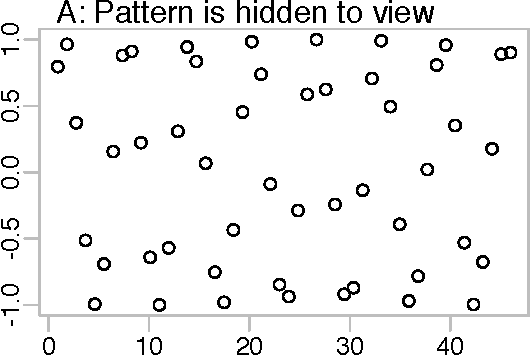
\includegraphics[width=0.48\linewidth]{03-graphs_files/figure-latex/Banking-1} 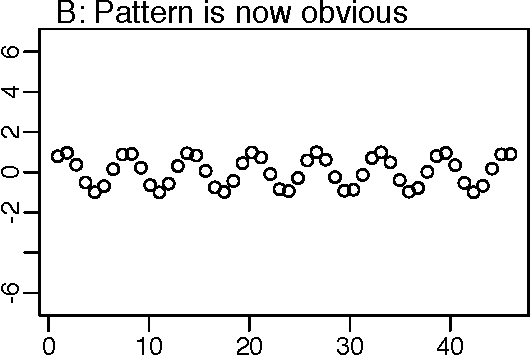
\includegraphics[width=0.48\linewidth]{03-graphs_files/figure-latex/Banking-2} \caption{The same data are used for both graphs.  The pattern that is not
obvious in Panel A is very obvious in Panel B}\label{fig:Banking}
\end{figure}

\hypertarget{varying-time-intervals-show-rates-not-counts}{%
\section{Varying time intervals --- show rates, not counts}\label{varying-time-intervals-show-rates-not-counts}}

\begin{Shaded}
\begin{Highlighting}[]
\FunctionTok{par}\NormalTok{(}\AttributeTok{mar=}\FunctionTok{c}\NormalTok{(}\FloatTok{4.1}\NormalTok{,}\FloatTok{3.1}\NormalTok{,}\FloatTok{2.1}\NormalTok{,}\FloatTok{3.1}\NormalTok{),}\AttributeTok{mgp=}\FunctionTok{c}\NormalTok{(}\FloatTok{2.25}\NormalTok{,}\FloatTok{0.5}\NormalTok{,}\DecValTok{0}\NormalTok{))}
\NormalTok{n2 }\OtherTok{\textless{}{-}} \FunctionTok{c}\NormalTok{(}\DecValTok{1}\NormalTok{,}\DecValTok{1}\NormalTok{,}\DecValTok{4}\NormalTok{,}\DecValTok{12}\NormalTok{,}\DecValTok{15}\NormalTok{,}\DecValTok{29}\NormalTok{,}\DecValTok{27}\NormalTok{,}\DecValTok{11}\NormalTok{)}
\NormalTok{n1 }\OtherTok{\textless{}{-}} \FunctionTok{c}\NormalTok{(}\DecValTok{1}\NormalTok{,}\DecValTok{1}\NormalTok{,}\DecValTok{4}\NormalTok{,}\DecValTok{12}\NormalTok{,}\DecValTok{15}\NormalTok{,}\DecValTok{29}\NormalTok{,}\DecValTok{27}\NormalTok{,}\DecValTok{39}\NormalTok{)}
\FunctionTok{plot}\NormalTok{(}\DecValTok{1}\SpecialCharTok{:}\DecValTok{8}\NormalTok{, n2, }\AttributeTok{xaxt=}\StringTok{"n"}\NormalTok{, }\AttributeTok{xlab=}\StringTok{""}\NormalTok{, }\AttributeTok{ylim=}\FunctionTok{range}\NormalTok{(n1),}
     \AttributeTok{ylab=}\StringTok{"Number of Nobel prizes"}\NormalTok{, }\AttributeTok{type=}\StringTok{"l"}\NormalTok{, }\AttributeTok{fg=}\StringTok{\textquotesingle{}gray\textquotesingle{}}\NormalTok{)}
\FunctionTok{axis}\NormalTok{(}\DecValTok{1}\NormalTok{, }\AttributeTok{at=}\DecValTok{1}\SpecialCharTok{:}\DecValTok{8}\NormalTok{, }\AttributeTok{labels=}\FunctionTok{paste0}\NormalTok{(}\FunctionTok{seq}\NormalTok{(}\AttributeTok{from=}\DecValTok{1901}\NormalTok{, }\AttributeTok{to=}\DecValTok{1971}\NormalTok{, }\AttributeTok{by=}\DecValTok{10}\NormalTok{),}\StringTok{"{-}"}\NormalTok{), }\AttributeTok{cex.axis=}\FloatTok{0.9}\NormalTok{, }\AttributeTok{gap.axis=}\FloatTok{0.15}\NormalTok{)}
\FunctionTok{axis}\NormalTok{(}\DecValTok{1}\NormalTok{, }\AttributeTok{at=}\DecValTok{1}\SpecialCharTok{:}\DecValTok{8}\NormalTok{, }\AttributeTok{labels=}\FunctionTok{paste0}\NormalTok{(}\FunctionTok{c}\NormalTok{(}\FunctionTok{seq}\NormalTok{(}\AttributeTok{from=}\DecValTok{1910}\NormalTok{, }\AttributeTok{to=}\DecValTok{1970}\NormalTok{, }\AttributeTok{by=}\DecValTok{10}\NormalTok{),}\DecValTok{1974}\NormalTok{)),}
     \AttributeTok{line=}\FloatTok{0.8}\NormalTok{, }\AttributeTok{lty=}\DecValTok{0}\NormalTok{, }\AttributeTok{cex.axis=}\FloatTok{0.9}\NormalTok{)}
\FunctionTok{axis}\NormalTok{(}\DecValTok{1}\NormalTok{, }\AttributeTok{at=}\DecValTok{1}\SpecialCharTok{:}\DecValTok{7}\NormalTok{, }\AttributeTok{labels=}\ConstantTok{FALSE}\NormalTok{)}
\FunctionTok{mtext}\NormalTok{(}\AttributeTok{side=}\DecValTok{3}\NormalTok{, }\AttributeTok{line=}\FloatTok{0.5}\NormalTok{, }\AttributeTok{at=}\FloatTok{0.5}\NormalTok{, }\StringTok{"Total prizes (black line)"}\NormalTok{, }\AttributeTok{adj=}\DecValTok{0}\NormalTok{, }\AttributeTok{cex=}\FloatTok{1.25}\NormalTok{)}
\FunctionTok{mtext}\NormalTok{(}\AttributeTok{side=}\DecValTok{3}\NormalTok{, }\AttributeTok{line=}\FloatTok{0.5}\NormalTok{, }\AttributeTok{at=}\FloatTok{8.5}\NormalTok{, }\StringTok{"Average prizes per year (blue dots)"}\NormalTok{, }\AttributeTok{col=}\StringTok{\textquotesingle{}blue\textquotesingle{}}\NormalTok{, }\AttributeTok{adj=}\DecValTok{1}\NormalTok{, }\AttributeTok{cex=}\FloatTok{1.25}\NormalTok{)}
\FunctionTok{points}\NormalTok{(}\DecValTok{1}\SpecialCharTok{:}\DecValTok{8}\NormalTok{, n1, }\AttributeTok{lwd=}\DecValTok{8}\NormalTok{, }\AttributeTok{col=}\FunctionTok{adjustcolor}\NormalTok{(}\StringTok{\textquotesingle{}blue\textquotesingle{}}\NormalTok{, }\AttributeTok{alpha=}\FloatTok{0.5}\NormalTok{), }\AttributeTok{pch=}\DecValTok{1}\NormalTok{)}
\FunctionTok{lines}\NormalTok{(}\DecValTok{7}\SpecialCharTok{:}\DecValTok{8}\NormalTok{, }\FunctionTok{tail}\NormalTok{(n1,}\DecValTok{2}\NormalTok{), }\AttributeTok{lty=}\DecValTok{2}\NormalTok{,}\AttributeTok{lwd=}\DecValTok{2}\NormalTok{, }\AttributeTok{col=}\FunctionTok{adjustcolor}\NormalTok{(}\StringTok{\textquotesingle{}blue\textquotesingle{}}\NormalTok{, }\AttributeTok{alpha=}\FloatTok{0.5}\NormalTok{))}
\FunctionTok{axis}\NormalTok{(}\DecValTok{4}\NormalTok{, }\AttributeTok{at=}\NormalTok{(}\DecValTok{0}\SpecialCharTok{:}\DecValTok{4}\NormalTok{)}\SpecialCharTok{*}\DecValTok{10}\NormalTok{, }\AttributeTok{labels=}\FunctionTok{paste}\NormalTok{(}\DecValTok{0}\SpecialCharTok{:}\DecValTok{4}\NormalTok{), }\AttributeTok{col.ticks=}\FunctionTok{adjustcolor}\NormalTok{(}\StringTok{\textquotesingle{}blue\textquotesingle{}}\NormalTok{, }\AttributeTok{alpha=}\FloatTok{0.5}\NormalTok{), }\AttributeTok{col.axis=}\StringTok{\textquotesingle{}blue\textquotesingle{}}\NormalTok{)}
\FunctionTok{mtext}\NormalTok{(}\AttributeTok{side=}\DecValTok{4}\NormalTok{, }\AttributeTok{line=}\FloatTok{1.8}\NormalTok{, }\StringTok{"Nobel prizes per year"}\NormalTok{, }\AttributeTok{col=}\StringTok{\textquotesingle{}blue\textquotesingle{}}\NormalTok{)}
\end{Highlighting}
\end{Shaded}

\begin{figure}[H]
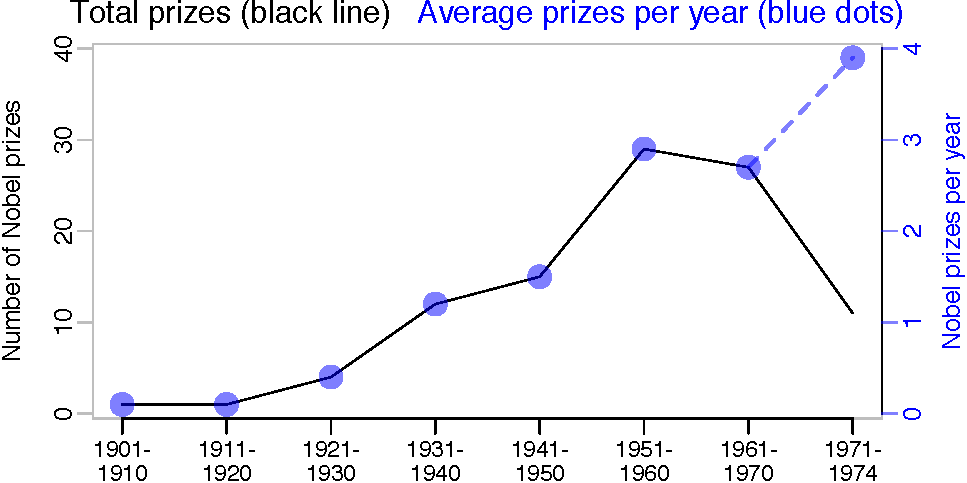
\includegraphics[width=0.8\linewidth]{03-graphs_files/figure-latex/Nobel-1} \caption{The black line shows numbers of US Nobel prizes, for given time intervals.
The blue dots show average number per year, as indicated by the axis on the right.}\label{fig:Nobel}
\end{figure}

A graph that was essentially the black segmented line in Figure
\ref{fig:Nobel} appeared in
\citet{national1975science} ``Science Indicators, 1974''. The segmented line gives
a highly misleading impression for the four years 1971-1974, as
opposed to earlier points, where numbers are totals over decades.
It joins up a final point that is a different measure from earlier
points.

A proper comparison between the number of Nobel prizes
in the earlier decades and the number in the four-year
period 1971-1974 adjusts for the length of time (ten years
versus four years) to which the count relates. The blue
dots, and the axis on the right, fairly represent change
over time.

The same principle applies for intervals of measures
other than time --- for example of length or volume.

\enlargethispage{13pt}

\hypertarget{helpful-web-links-are}{%
\section{Helpful web links are:}\label{helpful-web-links-are}}

\begin{itemize}
\tightlist
\item
  Good \& bad graphs (Murrell, lecture notes)\footnote{\url{https://www.stat.auckland.ac.nz/~ihaka/120/Lectures/lecture03.pdf}}
\item
  A short tour of bad graphs (Schwartz)\footnote{\textless www.stat.sfu.ca/\textasciitilde cschwarz/Stat-650/Notes/PDF/ChapterBadgraphs.pdf\textgreater{}}
\item
  Misleading graphs\footnote{\textless www.statisticshowto.com/misleading-graphs/\textgreater{}}

  \begin{itemize}
  \tightlist
  \item
    Color choices\footnote{\textless www.stonesc.com/pubs/Expert\%20Color\%20Choices.pdf\textgreater{}}
  \item
    Color Brewer\footnote{\textless www.statisticshowto.com/misleading-graphs/\textgreater{}}
  \end{itemize}
\end{itemize}

\hypertarget{selection-and-survivor-bias}{%
\chapter{Selection and survivor bias}\label{selection-and-survivor-bias}}

In mind here are cases where the data are not a random sample.

\hypertarget{the-hazards-of-convenience-samples}{%
\section{The hazards of convenience samples}\label{the-hazards-of-convenience-samples}}

Quota sampling has often been used as an alternative to random
sampling --- quotas are set for age categories, male/female,
and socioeconomic categories that are designed to ensure that
the sample~is representative of the wider population.
In polls~prior to the 1948 US presidential election that pitted
democrat Harry Truman against republican Thomas Dewey,
pollsters were given strict quotas, but otherwise left~free to
decide who they would approach. Polls by three different
organizations gave Dewey a lead of between 5\% and 15\%. In the
event, Truman led by 5\%.

\hypertarget{convenience-samples-sometimes-have-a-story-to-tell}{%
\subsection{Convenience samples sometimes have a story to tell}\label{convenience-samples-sometimes-have-a-story-to-tell}}

This is no to rule out all use of convenience samples.
Convenience samples, taken within a limited population, can
sometimes be useful in setting a lower bound.
It is strongly in the public interest that scientists have
reasonable freedom for responsible expression of their minds
on issues of public concern. In an informal 2015 survey, 151
Crown Research Institute scientists (out of 384 who responded)
answered yes to the question ``Have you ever been prevented
from making a public comment on a controversial issue by your
management's policy, or by fear of losing research funding?''
The 384 who responded will undoubtedly be a biased sample.
Irrespective of the size of the bias, the number who had not
been allowed to speak their mind was large enough to be a cause
for serious concern. Hon Joyce's response, to the effect that
as this was not a scientific survey of all CRI scientists
(to this extent, true), its evidence of large concern could be
ignored, was an evasion. Equally disturbing was the reaction
of the NIWA management, suggesting that they did not accept a
responsibility to defend transparency.\footnote{See \url{https://sciblogs.co.nz/infectious-thoughts/2015/08/28/niwa-in-astonishing-attack-on-scientist-association/}}

\hypertarget{uk-cotton-worker-wages-in-the-1880s}{%
\section{UK cotton worker wages in the 1880s}\label{uk-cotton-worker-wages-in-the-1880s}}

Prior to the \citet{boot2008new} paper\footnote{``New estimates of age- and sex- specific
  earnings and the male-female earnings gap in the British cotton
  industry, 1833-1906''} the main source of published information on
cotton worker wages in the UK in the late 19th century were results
from an 1889 US Bureau of Labor survey, intended for~use for
comparison with the US cotton industry wages.
Figure \ref{fig:cotton} compares the US Bureau of Labor survey
numbers with 1886 census numbers of different types of full time
UK cotton operatives.

\begin{Shaded}
\begin{Highlighting}[]
\NormalTok{cap22 }\OtherTok{\textless{}{-}} \StringTok{"Cotton worker wages in the UK {-}{-}{-} 1889 US Bureau of Labor \textquotesingle{}survey\textquotesingle{}}
\StringTok{versus 1886 census data. Wages are in pence per week."}
\end{Highlighting}
\end{Shaded}

\begin{Shaded}
\begin{Highlighting}[]
\DocumentationTok{\#\# detach("package:latticeExtra")}
\FunctionTok{suppressPackageStartupMessages}\NormalTok{(}\FunctionTok{library}\NormalTok{(ggplot2, }\AttributeTok{quietly=}\ConstantTok{TRUE}\NormalTok{))}
\NormalTok{cottonworkers }\OtherTok{\textless{}{-}}\NormalTok{ DAAG}\SpecialCharTok{::}\NormalTok{cottonworkers}
\FunctionTok{names}\NormalTok{(cottonworkers)[}\DecValTok{3}\NormalTok{] }\OtherTok{\textless{}{-}} \StringTok{"Av\_wage"}
\NormalTok{cottonworkers}\SpecialCharTok{$}\NormalTok{occ }\OtherTok{\textless{}{-}} \FunctionTok{row.names}\NormalTok{(cottonworkers)}
\NormalTok{cottonworkers}\SpecialCharTok{$}\NormalTok{occ[cottonworkers}\SpecialCharTok{$}\NormalTok{census1886}\SpecialCharTok{\textless{}}\DecValTok{2500}\NormalTok{] }\OtherTok{\textless{}{-}} \StringTok{""}
\NormalTok{cottonworkers}\SpecialCharTok{$}\NormalTok{occ2 }\OtherTok{\textless{}{-}} \FunctionTok{row.names}\NormalTok{(cottonworkers)}
\NormalTok{cottonworkers}\SpecialCharTok{$}\NormalTok{occ2[}\SpecialCharTok{!}\NormalTok{cottonworkers}\SpecialCharTok{$}\NormalTok{census1886 }\SpecialCharTok{\%in\%} \FunctionTok{c}\NormalTok{(}\DecValTok{208}\NormalTok{, }\DecValTok{1250}\SpecialCharTok{:}\DecValTok{2500}\NormalTok{)] }\OtherTok{\textless{}{-}} \StringTok{""}
\NormalTok{gph }\OtherTok{\textless{}{-}} \FunctionTok{ggplot}\NormalTok{(cottonworkers,}
              \FunctionTok{aes}\NormalTok{(census1886,survey1889,}\AttributeTok{label=}\NormalTok{occ,}
                  \AttributeTok{size=}\NormalTok{Av\_wage, }\AttributeTok{hjust=}\DecValTok{1}\NormalTok{))}\SpecialCharTok{+} 
  \FunctionTok{geom\_abline}\NormalTok{(}\AttributeTok{intercept=}\DecValTok{0}\NormalTok{, }\AttributeTok{slope=}\FloatTok{0.00986}\NormalTok{, }\AttributeTok{color=}\StringTok{"gray"}\NormalTok{) }\SpecialCharTok{+}
  \FunctionTok{geom\_point}\NormalTok{()}\SpecialCharTok{+}
  \FunctionTok{geom\_text}\NormalTok{(}\AttributeTok{size=}\DecValTok{4}\NormalTok{,}\AttributeTok{nudge\_x=}\SpecialCharTok{{-}}\DecValTok{180}\NormalTok{) }\SpecialCharTok{+}
  \FunctionTok{geom\_text}\NormalTok{(}\FunctionTok{aes}\NormalTok{(}\AttributeTok{y=}\NormalTok{survey1889}\SpecialCharTok{+}\FunctionTok{rep}\NormalTok{(}\FunctionTok{c}\NormalTok{(}\DecValTok{5}\NormalTok{,}\SpecialCharTok{{-}}\DecValTok{5}\NormalTok{),}\FunctionTok{c}\NormalTok{(}\DecValTok{7}\NormalTok{,}\DecValTok{7}\NormalTok{)), }\AttributeTok{label=}\NormalTok{occ2), }
            \AttributeTok{size=}\DecValTok{4}\NormalTok{, }\AttributeTok{hjust=}\DecValTok{0}\NormalTok{, }\AttributeTok{nudge\_x=}\DecValTok{100}\NormalTok{) }\SpecialCharTok{+}
  \FunctionTok{xlab}\NormalTok{(}\StringTok{"Number in 1886 census"}\NormalTok{) }\SpecialCharTok{+} \FunctionTok{ylab}\NormalTok{(}\StringTok{"Number in 1889 survey"}\NormalTok{)}
\NormalTok{leg }\OtherTok{\textless{}{-}} \FunctionTok{matrix}\NormalTok{(}\FunctionTok{c}\NormalTok{(}\StringTok{"The line shows what 1899"}\NormalTok{,}
                \StringTok{"survey numbers would be,"}\NormalTok{,}
                \StringTok{"if relative numbers in"}\NormalTok{,}
                \StringTok{"worker categories were"}\NormalTok{,}
                \StringTok{"as in the 1886 census"}\NormalTok{), }\AttributeTok{ncol=}\DecValTok{1}\NormalTok{)}
\FunctionTok{library}\NormalTok{(gridExtra)}
\NormalTok{tt }\OtherTok{\textless{}{-}} \FunctionTok{ttheme\_minimal}\NormalTok{(}\AttributeTok{base\_size=}\DecValTok{12}\NormalTok{, }
                     \AttributeTok{core =} \FunctionTok{list}\NormalTok{(}\AttributeTok{fg\_params=}\FunctionTok{list}\NormalTok{(}\AttributeTok{hjust =} \DecValTok{0}\NormalTok{, }\AttributeTok{x=}\DecValTok{0}\NormalTok{)))}
\NormalTok{gph }\SpecialCharTok{+} \FunctionTok{annotation\_custom}\NormalTok{(}\FunctionTok{tableGrob}\NormalTok{(leg, }\AttributeTok{theme=}\NormalTok{tt), }
                       \AttributeTok{xmax=}\DecValTok{3600}\NormalTok{, }\AttributeTok{ymin=}\DecValTok{100}\NormalTok{, }\AttributeTok{ymax=}\DecValTok{150}\NormalTok{)}
\end{Highlighting}
\end{Shaded}

\begin{figure}
\centering
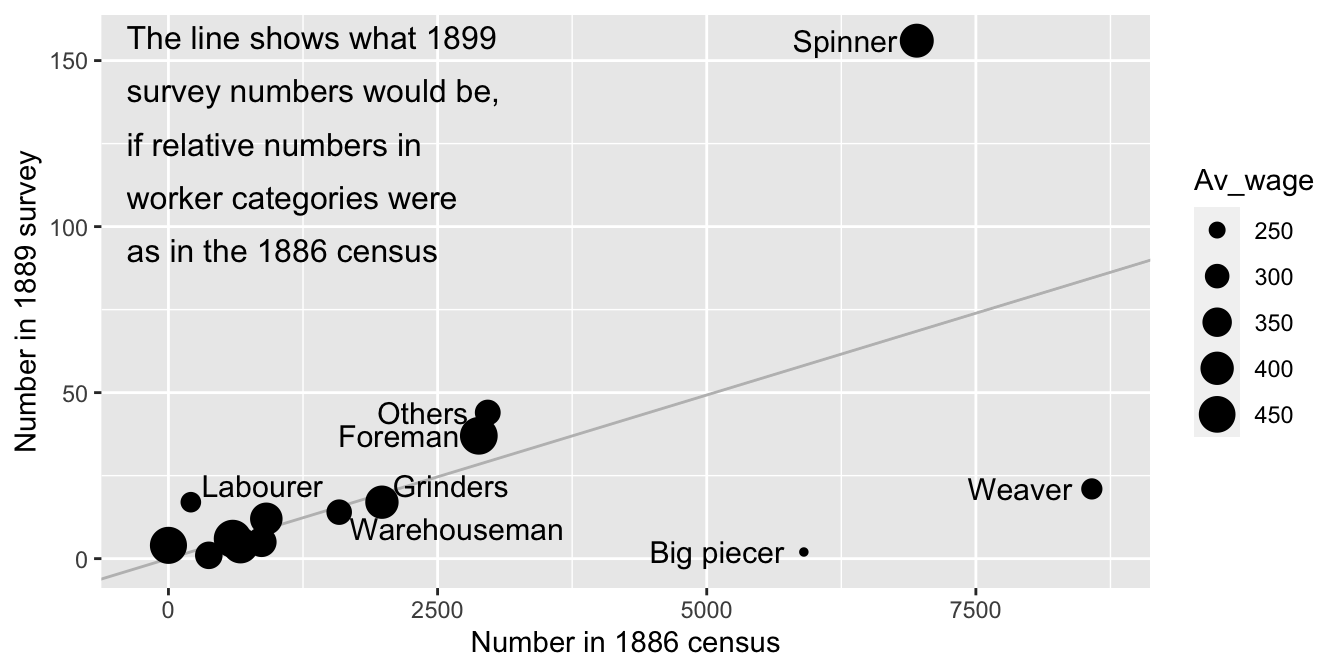
\includegraphics{04-select_files/figure-latex/cotton-1.pdf}
\caption{\label{fig:cotton}Cotton worker wages in the UK --- 1889 US Bureau of Labor `survey'
versus 1886 census data. Wages are in pence per week.}
\end{figure}

The 1889 survey shows some strong biases --- a result it
would seem of geographical bias and of the informal data
collection methods that were used. The high wages given to
spinners were grossly over-weighted in the US Bureau of
Labor survey, while Big Piecers and Weavers were grossly
under-represented. A guess is that workers were asked for
information on their wages as they left work, and that
the survey personnel happened to catch employees at a time
when there was a large preponderance of highly paid spinners,
and an untypically small number of big piecers and weavers.
The net effect was a gross over-estimate of average wages.

\hypertarget{how-good-a-guide-does-the-past-provide-to-the-future}{%
\section{How good a guide does the past provide to the future?}\label{how-good-a-guide-does-the-past-provide-to-the-future}}

There is a mix of selection and survivor bias arise when data
from the past are used as a guide to the future, with no
allowance for the source/target difference. The target about
which we wish to~make judgments lies in the future, while the
data are from the past. Think about a business that is
planning for the future. One can never know, until after the
event, all the ramifications of the choices made.

Businesses may be selected as examples of effective business
practice because they were, at the time when the data were
collated, successful. Likewise, it is athletes who have
been successful in the recent past who are likely to be
selected to~appear on the covers of sports magazines.
In either case, this gives a biased picture of what can be
expected in the future --- in many cases those who are
picked out will be close to~the peak of their success,
and/or have had unusual luck. High levels of success in
the recent past will not always translate into success
in the following year or years. How often will past
success translate into future success? In order to
discover, it is necessary to collect relevant data.

Subsection \ref{ss:wald} will discuss a widely cited example
of survivor bias that relates to the relative density
of bullet holes, in different parts of the plane, in planes
that had returned from battle in World War II. The key to
interpreting the data was to recognize that these were the
planes that had survived.

\hypertarget{tales-of-standout-past-success-pp.3839}{%
\section{Tales of standout past success (pp.38--39)}\label{tales-of-standout-past-success-pp.3839}}

\hypertarget{collins_2001-good-to-great}{%
\subsection*{\texorpdfstring{\citet{collins_2001} --- Good to Great}{@collins\_2001 --- Good to Great}}\label{collins_2001-good-to-great}}
\addcontentsline{toc}{subsection}{\citet{collins_2001} --- Good to Great}

\begin{itemize}
\tightlist
\item
  From 1,435 companies, Collins identified 11 as standouts

  \begin{itemize}
  \tightlist
  \item
    Since 2001, 5 better than average; 6 worse
  \item
    Fannie Mae --- 2001: \textgreater\$80 per share: 2008: \textless\$1
  \item
    Circuit City: Bankrupt in 2009
  \end{itemize}
\end{itemize}

\hypertarget{waterman1982search-in-search-of-excellence}{%
\subsection*{\texorpdfstring{\citet{waterman1982search} --- In Search of Excellence}{@waterman1982search --- In Search of Excellence}}\label{waterman1982search-in-search-of-excellence}}
\addcontentsline{toc}{subsection}{\citet{waterman1982search} --- In Search of Excellence}

\begin{itemize}
\tightlist
\item
  43 successful companies:

  \begin{itemize}
  \tightlist
  \item
    ``Bias for action''; ``Close to consumer''
  \end{itemize}
\item
  From the 35 that were publicly listed:

  \begin{itemize}
  \tightlist
  \item
    Since 1982: 15 better than average; 20 worse
  \end{itemize}
\end{itemize}

In all cases, companies that were chosen as examples of
standout success were likely to be near to~the peak of
their performance, as judged by Collins, or by Waterman and Peters.
Overlaid on this is the regression effect that will be discussed
in Chapter \ref{sec:reg}.

\hypertarget{ss:wald}{%
\section{Damaged planes --- how were the data generated?}\label{ss:wald}}

Abraham Wald's insight was that survivor bias was to be
expected, with the density of bullet~holes providing evidence
about the extent of bias, and the implications for identifying
the part(s) of the planes that would benefit most from
additional protection. See \href{https://medium.com/@penguinpress/an-excerpt-from-how-not-to-be-wrong-by-jordan-ellenberg-664e708cfc3d}{Abraham Wald and the Missing Bullet Holes}\footnote{\url{https://medium.com/@penguinpress/an-excerpt-from-how-not-to-be-wrong-by-jordan-ellenberg-664e708cfc3d}},
which is~an excerpt from \citet{ellenberg_2015}.

The~numbers of hits per square foot were:

\begin{Shaded}
\begin{Highlighting}[]
\FunctionTok{c}\NormalTok{(}\StringTok{\textquotesingle{}Engines\textquotesingle{}}\OtherTok{=}\FloatTok{1.11}\NormalTok{, }\StringTok{"Fusilage"}\OtherTok{=}\FloatTok{1.73}\NormalTok{,}\StringTok{"Fuel system"}\OtherTok{=}\FloatTok{1.55}\NormalTok{, }\StringTok{"Rest of plane"}\OtherTok{=}\FloatTok{1.8}\NormalTok{)}
\end{Highlighting}
\end{Shaded}

\begin{verbatim}
##       Engines      Fusilage   Fuel system Rest of plane 
##          1.11          1.73          1.55          1.80
\end{verbatim}

It was not possible to fit protective plates everywhere,
as this would~have made the planes overly heavy? Wald argued
that the holes very likely were spread pretty much uniformly
over the planes as a whole, those that were shot down, and those
that survived, The reason for relatively fewer bullet holes in
the engine and fuel system areas was that hits in those areas
were more likely to bring the plane down, so~that they did not
return.

\hypertarget{medical-and-related-tests-and-trials}{%
\chapter{Medical and related tests and trials}\label{medical-and-related-tests-and-trials}}

\hypertarget{useful-general-sources-of-advice-and-information}{%
\section{Useful general sources of advice and information}\label{useful-general-sources-of-advice-and-information}}

\hypertarget{the-harding-center-for-risk-literacy}{%
\subsection*{The Harding Center for Risk Literacy}\label{the-harding-center-for-risk-literacy}}
\addcontentsline{toc}{subsection}{The Harding Center for Risk Literacy}

There is extensive informative content on the \href{https://www.hardingcenter.de/en}{Harding Center for Risk Literacy site}\footnote{\url{https://www.hardingcenter.de/en}} site. Note, in particular:

\begin{itemize}
\tightlist
\item
  \href{https://www.hardingcenter.de/en/team}{Team}\footnote{\url{https://www.hardingcenter.de/en/team}}
\item
  \href{https://www.hardingcenter.de/en/transfer-and-impact/fact-boxes}{Medical Fact Boxes}
\item
  \href{https://www.hardingcenter.de/en/the-harding-center/publications/scientific-publications}{Publications}
\item
  \href{https://www.hardingcenter.de/en/harding-center/media}{In the Media}
\end{itemize}

\hypertarget{harding-center-medical-fact-boxes}{%
\subsection*{Harding Center Medical Fact Boxes}\label{harding-center-medical-fact-boxes}}
\addcontentsline{toc}{subsection}{Harding Center Medical Fact Boxes}

Medical fact boxes\footnote{\url{https://www.hardingcenter.de/en/projects-and-collaborations/fact-boxes}} provide visual and tabular summaries of the current
``best'' evidence, from randomized controlled trials. The comparison
may be with a placebo, or with an alternative that is known to be
effective. Detailed references are given. Where available, reliance
is on Cochrane studies. Some of the available fact boxes are:

\begin{itemize}
\tightlist
\item
  \href{https://www.hardingcenter.de/en/projects-and-collaborations/fact-boxes/early-detection-cancer}{Early cancer detection: breast, ovarian, prostate, colon, cervix}
\item
  \href{https://www.hardingcenter.de/en/projects-and-collaborations/fact-boxes/cardiovascular-diseases}{Cardiovascular Diseases}
\item
  \href{https://www.hardingcenter.de/en/projects-and-collaborations/fact-boxes/vaccines}{Vaccines}
\item
  \href{https://www.hardingcenter.de/en/projects-and-collaborations/fact-boxes/imaging-tests-low-back-pain}{Low back pain}
\item
  \href{https://www.hardingcenter.de/en/projects-and-collaborations/fact-boxes/osteoarthritis-knee}{Osteoarthritis of the knee}
\item
  \href{https://www.hardingcenter.de/en/projects-and-collaborations/fact-boxes/dietary-supplements}{Dietary Supplements - Selenium}
\end{itemize}

Note also

\begin{itemize}
\tightlist
\item
  \href{https://www.hardingcenter.de/en/transfer-and-impact/what-you-should-know-about-sars-cov-2-and-covid-19}{information material on SARS-CoV-2 and Covid-19}\footnote{\url{https://www.hardingcenter.de/en/transfer-and-impact/what-you-should-know-about-sars-cov-2-and-covid-19}}
\item
  \href{https://docs.google.com/forms/d/e/1FAIpQLSfw3Pe5a_g6lALY7ad3Aq7fBu2Sro4uteUKqvvvCARICxOQ9g/viewform?usp=sf_link}{Are you risk literate? --- Risk quiz}\footnote{\url{https://docs.google.com/forms/d/e/1FAIpQLSfw3Pe5a_g6lALY7ad3Aq7fBu2Sro4uteUKqvvvCARICxOQ9g/viewform?usp=sf_link}}
\end{itemize}

\hypertarget{other-sources-of-information}{%
\section{Other sources of information}\label{other-sources-of-information}}

\begin{itemize}
\tightlist
\item
  Winton Centre for Risk and Evidence Communication\footnote{\url{https://wintoncentre.maths.cam.ac.uk/}}
\item
  {[}US Consumer health information site\footnote{\url{https://medlineplus.gov/}}
\end{itemize}

\hypertarget{the-cochrane-center}{%
\subsection*{\texorpdfstring{The Cochrane Center\footnote{\url{https://www.cochrane.org/}}}{The Cochrane Center}}\label{the-cochrane-center}}
\addcontentsline{toc}{subsection}{The Cochrane Center}

The Cochrane Center's mission is ``to promote evidence-informed health decision-making by producing high-quality, relevant, accessible systematic
reviews and other synthesized research evidence.'' They rely heavily on
meta-analyses, looking for the balance of evidence across all relevant
studies.

\hypertarget{psa-screening-for-prostate-cancer-and-more}{%
\section{PSA Screening for Prostate Cancer, and more}\label{psa-screening-for-prostate-cancer-and-more}}

Numbers (rounded) in the following table are from a Harding Center
fact box. They are for men 50 years or older who either did or did not
participate in prostate cancer screening, using the PSA test, for 16 years.\footnote{\url{https://www.hardingcenter.de/en/early-detection-of-cancer/early-detection-of-prostate-cancer-with-psa-testing}}

\begin{longtable}[]{@{}lll@{}}
\toprule
& 1000 men, No screening & 1000 men, Screening \\
\midrule
\endhead
Deaths (any cause) & 322 & 322 \\
Deaths (prostate cancer) & 12 & 10 \\
& & \\
Biopsy \& false alarm & 0 & 155 \\
Unnecessary treatment & 0 & 51 \\
\bottomrule
\end{longtable}

About 10 out of every 1,000 men with screening, and 12 out of every 1,000 men without screening died from prostate cancer within 16 years. This means that 2 out of every 1,000 people could be saved from death from prostate cancer by early detection using PSA testing. This was not reflected in overall mortality.

Numbers for benefits are based on four studies with about 77,000 participants (progressive cancer), four studies with about 472,000 participants (overall mortality), and eleven studies with about 619,000 participants (prostate cancer specific mortality). The numbers for harms are based on seven studies with approximately 128,000 participants (false-positive results within three to six participations in PSA testing for early detection) and nine studies with approximately 274,000 participants (over-diagnosis and over-treatment). See
the web site for references to the studies.

Unlike the biopsies that may follow a positive PSA test, the PSA test has
no direct potential to cause physical harm. The harm results from an
undue readiness to use the test result as a reason for further testing
and treatment that will in many cases itself cause harm. ``Wait and watch''
appears the preferred strategy.

See also: \citet{levitin_2015}, Chapter 6, and
\href{https://www.nytimes.com/2011/10/09/books/review/your-medical-mind-by-jerome-groopman-and-pamela-hartzband-book-review.html}{How Patients Think, and How They Should}\footnote{\url{https://www.nytimes.com/2011/10/09/books/review/your-medical-mind-by-jerome-groopman-and-pamela-hartzband-book-review.html}}

\hypertarget{ss:rct}{%
\section{Randomized Controlled Trials (RCTs) versus Population Studies}\label{ss:rct}}

Two types of study are widely used in medical and other contexts ---
randomized controlled trials, and population-based studies.
These can, in both cases, be broken down into further sub-types.
There may be elements of both these types of studies.

\hypertarget{randomized-controlled-trials-rcts-the-gold-standard}{%
\subsection*{Randomized Controlled Trials (RCTs) --- the gold standard?}\label{randomized-controlled-trials-rcts-the-gold-standard}}
\addcontentsline{toc}{subsection}{Randomized Controlled Trials (RCTs) --- the gold standard?}

\begin{itemize}
\tightlist
\item
  Ensure that apples are compared with apples

  \begin{itemize}
  \tightlist
  \item
    Use a random mechanism to assign to assign to treatment as
    against control --- in a medical screening study to
    ``screen'' or ``not screen''
  \item
    Treatment and control must otherwise be treated in the
    same way.
  \end{itemize}
\item
  There must be strict adherence to a protocol

  \begin{itemize}
  \tightlist
  \item
    Minor departures that may, e.g., allow unconscious bias
    in the way that results from the different groups of participants
    are measured, can invalidate results.
  \end{itemize}
\item
  Results apply, strictly, to those who meet the trial entry criteria

  \begin{itemize}
  \tightlist
  \item
    This may limit relevance to general population
  \end{itemize}
\end{itemize}

Especially in medical trials, think carefully about the outcome measure.

\begin{itemize}
\tightlist
\item
  In a screening trial, e.g., for prostate cancer, there are
  risks both for those who test positive, and for
  those who test negative.

  \begin{itemize}
  \tightlist
  \item
    The process used to check for cancer may itself bring
    a smaller or larger element of risk.
  \item
    Positives may be false positives, leading to more invasive
    checks which~may themselves carry a risk. Thus, for prostate
    cancer, a positive PSA test is likely to lead to a biopsy that
    itself has been estimated to carry a 5\% risk of serious side
    effects, with a much higher proportion of less serious effects
    \citep[p.245]{levitin_2015}
  \item
    Some slow growing cancers may be better left untreated,
    rather than exposing the patient to a treatment that may itself
    do serious damage.
  \end{itemize}
\item
  Thus, think carefully about the choice of outcome measure. It is not
  enough to show that a screening program will pick up otherwise
  undiagnosed cancers.
\end{itemize}

For a helpful animated summary of some of the key issues, see:\\
\url{https://www.youtube.com/watch?v=Wy7qpJeozec}

\hypertarget{a-note-in-passing-hippo-decisions-vs-ab-testing}{%
\subsection*{A note in passing: HiPPO decisions vs A/B testing}\label{a-note-in-passing-hippo-decisions-vs-ab-testing}}
\addcontentsline{toc}{subsection}{A note in passing: HiPPO decisions vs A/B testing}

Randomized studies are widely used outside of medicine.
Randomization is a key component of the way that Google and
others test out, e.g., the effect of different web page layouts.

\begin{itemize}
\tightlist
\item
  HiPPO = ``Highest paid person in the Office.''
\item
  The term ``A/B testing'' is sometimes used to refer to randomized
  testing of alternatives.
\end{itemize}

A/B testing helped propel Obama into office! An experiment was
conducted that involved 15 million people, or~about 25\%, from
its email list. The signup forms had one of nine different
combinations of images with words on which recipients were
invited to click, thus:

\begin{tabular}{lccc}
& Learn more & Join us & Sign up now \\
Obama photo & \ding{56} & \ding{56} & \ding{56} \\
BW photo of Obama family & \ding{52} & \ding{56} & \ding{56} \\
Obama speaking & \ding{56} & \ding{56} & \ding{56} \\
\end{tabular}

The black and white photo of the Obama family, with the words
``Learn more'', generated the most clicks.

\citet{young2014improving} gives an account of A/B testing as it might
be used for improving library user experience.

\hypertarget{population-studies-groups-must-be-broadly-comparable}{%
\subsection*{Population studies --- groups must be broadly comparable}\label{population-studies-groups-must-be-broadly-comparable}}
\addcontentsline{toc}{subsection}{Population studies --- groups must be broadly comparable}

\begin{itemize}
\tightlist
\item
  Adjust prunes to look like apples (is it possible?)
\item
  Can one ever be sure that the adjustments do the job?
\item
  Potential for biases is greater than for RCTs
\end{itemize}

Where a treatment is compared with a control group, the
idea is to use a regression type approach to adjust for
differences in such variables or factors as age, sex,
socioeconomic status, and co-morbidities.
``Propensity score'' approaches try to summarize such group
differences in a single variable (or, in principle, two
or more variables) that measure the propensity
to~belong to the treatment as opposed to the control group.
While their effectiveness for this purpose may be doubted,
they can be used to provide insightful graphs that check
the extent to which the groups are broadly comparable on
the variables and/or factors used to adjust for differences.

\hypertarget{issues-for-all-types-of-study}{%
\subsection*{Issues for all types of study}\label{issues-for-all-types-of-study}}
\addcontentsline{toc}{subsection}{Issues for all types of study}

What are the relevant outcome measures?

\begin{itemize}
\tightlist
\item
  e.g., cancer -- malignancies found \& removed, or deaths

  \begin{itemize}
  \tightlist
  \item
    deaths from cancer, or from all causes (for some individuals,
    the treatment may be more damaging in it medium to long term effect
    than the cancer)
  \end{itemize}
\end{itemize}

Care is required to deal with survivor, as well as other, biases.

\hypertarget{avoid-or-expose-infants-to-peanuts}{%
\section{Avoid, or expose infants~to~peanuts?}\label{avoid-or-expose-infants-to-peanuts}}

Clinical practice guidelines introduced in or around the
year 2000 had ``recommended the exclusion of
allergenic foods from the diets of infants at high risk for
allergy, and from the diets of their mothers during pregnancy
and lactation.''

It was then a surprise to find that
the prevalence of peanut allergy has substantially increased
in the recent past, doubling in Europe between 2005 and 2015,
suggesting that advice given to parents of young children to
avoid foods containing peanuts may have been counterproductive.
This reassessment was supported, at least for infants who
at four months had either severe eczema or food allergy or
both, and thus were at high risk of developing a peanut
allergy, by the LEAPS study reported in \citet{du2015randomized}.

As noted, the LEAPS study was limited to infants who at four
months had either severe eczema or food allergy or both.\\
Infants were stratified into two groups following a skin-prick
test, with each group then randomized between those exposed
to peanut extract, and those not exposed.

Among 530 infants in the population who initially had negative results on the skin-prick test, the prevalence of peanut allergy at 60 months of age was 13.7\% (37/270) in the avoidance group and 1.8\% (5/272) in the consumption group.\footnote{There were twelve further infants in this group~whose results
  could not be evaluated.}
Among the 98 participants who initially had positive test results, the prevalence of peanut allergy was 35.3\% (18/51) in the avoidance group
and 10.6\% (5/47) in the consumption group. There was no
between-group difference of consequence in the incidence of
serious adverse events.

In both groups, numbers and percentages are for those who were assigned
to the group and whose results could be evaluated, whether or not they
followed the treatment protocol to which they were assigned. In technical
terms, these are results from an ``intention to treat'' analysis. Such an
analysis is designed to mirror what can be expected in practice --- not
everyone who starts off in one group will stick to~it. It answers
questions about what to do with subjects who did~not fully follow
the treatment to which they were assigned.

The results were followed, in 2016, by changes to guidelines that
recommended introduction of peanut and other allergenic foods
before 12 months. The assumption that avoiding early exposure to
peanuts would reduce risk of later development of peanut allergy
was, it was judged, likely wrong for all~infants.

\hypertarget{false-positives-smith-pp.98-99}{%
\section{False Positives (Smith, pp.98-99)}\label{false-positives-smith-pp.98-99}}

In contexts where the number of false positives is likely to be
high relative to the number of true positives, screening
programs may have serious downsides that outweigh the benefits.

\begin{itemize}
\tightlist
\item
  A test for marijuana has a 95\% accuracy (true positive) rate
\item
  Of those who test positive, what fraction are marijuana users?
\end{itemize}

Administer test to 10,000 employees --- 500 use, 9500 do not

\begin{Shaded}
\begin{Highlighting}[]
\NormalTok{tab }\OtherTok{\textless{}{-}} \FunctionTok{matrix}\NormalTok{(}\FunctionTok{c}\NormalTok{(}\DecValTok{475}\NormalTok{,}\DecValTok{475}\NormalTok{,}\DecValTok{950}\NormalTok{,}\DecValTok{25}\NormalTok{,}\DecValTok{9025}\NormalTok{,}\DecValTok{9050}\NormalTok{,}\DecValTok{500}\NormalTok{,}\DecValTok{9500}\NormalTok{,}\DecValTok{10000}\NormalTok{), }\AttributeTok{ncol=}\DecValTok{3}\NormalTok{, }\AttributeTok{nrow=}\DecValTok{3}\NormalTok{)}
\FunctionTok{dimnames}\NormalTok{(tab) }\OtherTok{\textless{}{-}} \FunctionTok{list}\NormalTok{(}\FunctionTok{c}\NormalTok{(}\StringTok{"User"}\NormalTok{,}\StringTok{"Not user"}\NormalTok{,}\StringTok{"Total"}\NormalTok{),}\FunctionTok{c}\NormalTok{(}\StringTok{"Test +ve"}\NormalTok{,}\StringTok{"Test {-}ve"}\NormalTok{,}\StringTok{"Total"}\NormalTok{))}
\NormalTok{tab }\OtherTok{\textless{}{-}}\NormalTok{ xtable}\SpecialCharTok{::}\FunctionTok{xtable}\NormalTok{(tab, }\AttributeTok{digits=}\DecValTok{0}\NormalTok{)}
\FunctionTok{print}\NormalTok{(tab,}\AttributeTok{type=}\StringTok{\textquotesingle{}latex\textquotesingle{}}\NormalTok{, }\AttributeTok{comment=}\ConstantTok{FALSE}\NormalTok{, }\AttributeTok{floating=}\ConstantTok{FALSE}\NormalTok{, }\AttributeTok{scalebox=}\FloatTok{1.0}\NormalTok{)}
\end{Highlighting}
\end{Shaded}

\scalebox{1}{
\begin{tabular}{rrrr}
  \hline
 & Test +ve & Test -ve & Total \\ 
  \hline
User & 475 & 25 & 500 \\ 
  Not user & 475 & 9025 & 9500 \\ 
  Total & 950 & 9050 & 10000 \\ 
   \hline
\end{tabular}
}

\begin{itemize}
\tightlist
\item
  Consider a test for excess iron syndrome that has \textasciitilde80\% accuracy\\
  Excess iron syndrome has the name ``haemochromatosis''. Again,
  administer it to 10,000 individuals, where 50 have the syndrome,
  9950 do~not (a rate of 1 in 200).
\end{itemize}

\begin{Shaded}
\begin{Highlighting}[]
\NormalTok{tab }\OtherTok{\textless{}{-}} \FunctionTok{matrix}\NormalTok{(}\FunctionTok{c}\NormalTok{(}\DecValTok{40}\NormalTok{,}\DecValTok{1990}\NormalTok{,}\DecValTok{2030}\NormalTok{,}\DecValTok{10}\NormalTok{,}\DecValTok{7960}\NormalTok{,}\DecValTok{7970}\NormalTok{,}\DecValTok{50}\NormalTok{,}\DecValTok{9950}\NormalTok{,}\DecValTok{7000}\NormalTok{), }\AttributeTok{ncol=}\DecValTok{3}\NormalTok{, }\AttributeTok{nrow=}\DecValTok{3}\NormalTok{)}
\FunctionTok{dimnames}\NormalTok{(tab) }\OtherTok{\textless{}{-}} \FunctionTok{list}\NormalTok{(}\FunctionTok{c}\NormalTok{(}\StringTok{"Haem..."}\NormalTok{,}\StringTok{"Not haem..."}\NormalTok{,}\StringTok{"Total"}\NormalTok{),}\FunctionTok{c}\NormalTok{(}\StringTok{"Test +ve"}\NormalTok{,}\StringTok{"Test {-}ve"}\NormalTok{,}\StringTok{"Total"}\NormalTok{))}
\NormalTok{tab }\OtherTok{\textless{}{-}}\NormalTok{ xtable}\SpecialCharTok{::}\FunctionTok{xtable}\NormalTok{(tab, }\AttributeTok{digits=}\DecValTok{0}\NormalTok{)}
\FunctionTok{print}\NormalTok{(tab,}\AttributeTok{type=}\StringTok{\textquotesingle{}latex\textquotesingle{}}\NormalTok{, }\AttributeTok{comment=}\ConstantTok{FALSE}\NormalTok{, }\AttributeTok{floating=}\ConstantTok{FALSE}\NormalTok{, }\AttributeTok{scalebox=}\FloatTok{1.0}\NormalTok{)}
\end{Highlighting}
\end{Shaded}

\scalebox{1}{
\begin{tabular}{rrrr}
  \hline
 & Test +ve & Test -ve & Total \\ 
  \hline
Haem... & 40 & 10 & 50 \\ 
  Not haem... & 1990 & 7960 & 9950 \\ 
  Total & 2030 & 7970 & 7000 \\ 
   \hline
\end{tabular}
}

\hypertarget{the-aspirin-story-randomized-trials}{%
\subsection*{The Aspirin story (randomized trials)}\label{the-aspirin-story-randomized-trials}}
\addcontentsline{toc}{subsection}{The Aspirin story (randomized trials)}

22,000 males, 1st 5 years of study: \url{http://nyti.ms/2rgjFO2}

\begin{longtable}[]{@{}lll@{}}
\toprule
& Placebo group & Aspirin group \\
\midrule
\endhead
Fatal heart attacks & 18 & 5 \\
Non-fatal heart attacks & 171 & 99 \\
\bottomrule
\end{longtable}

Later work: Benefits are limited to those with previous symptoms\\
2009 study: \url{https://www.theguardian.com/society/2009/aug/31/aspirin-british-heart-foundation}\\
Major bleeding episodes, requiring admission to hospital:\\
were 20 (1.2\%) in the placebo group; 34 (2\%) in aspirin group

Summary of current evidence: \url{http://mayocl.in/1cBM0ze}

\hypertarget{breast-cancer-screening-a-very-contested-area}{%
\section{Breast cancer screening --- a very contested area}\label{breast-cancer-screening-a-very-contested-area}}

See, e.g., \citet{raichand2017conclusions}. The review starts with the comment:

\begin{quote}
The recent controversy about using mammography to screen for breast cancer based on randomized controlled trials over 3 decades in Western countries has not only eclipsed the paradigm of evidence-based medicine, but also puts health decision-makers in countries where breast cancer screening is still being considered in a dilemma to adopt or abandon such a well-established screening modality.
\end{quote}

As with PSA screening for prostate cancer, the
\href{https://www.hardingcenter.de/en/early-detection-breast-cancer-mammography-screening}{Harding Center Fact Box for Mammography Screening}\footnote{\url{https://www.hardingcenter.de/en/early-detection-breast-cancer-mammography-screening}} is a good place to go for
an up to date summary of the evidence. Those who are convinced of
the virtues of screening may wish to challenge the evidence as presented
at the time of writing. On what grounds, however? It may be argued
that

\begin{itemize}
\tightlist
\item
  Improvements in medical procedures since the time of the trials
  on which the Fact Boxes are based may have changed the balance of
  risk.
\item
  The trials do not apply to New Zealand conditions.
\end{itemize}

Both cases require justification.

\hypertarget{fame-that-may-spill-over-into-notoriety}{%
\chapter{Fame that may spill over into notoriety}\label{fame-that-may-spill-over-into-notoriety}}

\hypertarget{the-mmr-measles-mumps-and-rubella-scandal}{%
\section{\texorpdfstring{\href{https://en.wikipedia.org/wiki/MMR_vaccine_controversy}{The MMR (measles, mumps, and rubella) scandal}}{The MMR (measles, mumps, and rubella) scandal}}\label{the-mmr-measles-mumps-and-rubella-scandal}}

Andrew Wakefield was the lead author of a study published in 1998,
based on just twelve children, that claimed to find indications
of a link between the MMR (measles, mumps, and rubella) vaccine
and autism. The journalist Brian Deer had a key role in
identifying issues with the work,~including fraudulent
manipulation of~the medical~evidence.

\begin{itemize}
\tightlist
\item
  Wakefield had multiple undeclared conflicts of interest
\item
  Funding came from a group of lawyers who were interested
  in possible personal injury lawsuits
\item
  It emerged that from 9 children said to have regressive autism

  \begin{itemize}
  \tightlist
  \item
    Only 1 had been diagnosed; 3 had no autism\\
  \item
    5 had developmental problems before the vaccine
  \end{itemize}
\end{itemize}

Wakefield's 1998 claims were widely reported

\begin{itemize}
\tightlist
\item
  Vaccination rates in the UK and Ireland dropped sharply
\item
  The incidence of measles and mumps increased, resulting
  in deaths and in severe and permanent injuries.
\end{itemize}

Wakefield was found guilty by the General Medical Council of serious professional misconduct in May 2010 and was struck off the Medical Register.\\
Following the initial claims in 1998, multiple large epidemiological studies failed to find any link between MMR and autism.

Fact boxes on the Harding site summarize evidence of the
effectiveness of the \href{https://www.hardingcenter.de/de/search/node?keys=mmr}{MMR vaccine}\footnote{\url{https://www.hardingcenter.de/de/search/node?keys=mmr}\textgreater{}}

\hypertarget{sally-clarks-disturbing-cot-death-experience}{%
\section{Sally Clark's disturbing cot death experience}\label{sally-clarks-disturbing-cot-death-experience}}

Sudden Infant Death (SID), also referred to as ``cot death'',
is the name given to the unexplained sudden death of very
young children. The story of Sally Clark's unfortunate brush
with the law, following the death of a second child, is
interesting, disturbing, and educational. Sally's experience
highlighted ways in which the UK legal system needed to take
on board issues that affect the use of medical evidence ---
issues of a type that can be important in medical research.

Meadow argued that ``unless proved otherwise, one cot death is tragic,
two is suspicious and three is murder.''
Was this an example of ``Too hard! Try something easier, and wrong!''
Or was it the triumph of assumed ``knowledge'' over hard evidence?

Following the ``cot death'' of the second of Sally Clark's two children,
Meadow gave evidence at her trial in 1999, and appeal
in 2000. Sally Clark was finally acquitted in 2003.

\begin{itemize}
\tightlist
\item
  Meadow gave 1 in 8,500 as cot death rate in affluent non-smoking families

  \begin{itemize}
  \tightlist
  \item
    Squared 8,500 to get odds of 73,000,000:1 against for two deaths.
  \item
    Meadow assumed, wrongly, that the probability of a death from
    natural causes was the same in all families.
  \item
    A first ``cot death'' is, in some families at least, evidence of a greater
    proneness to death from natural causes.
  \end{itemize}
\item
  Royal Statistical Society press release: ``Figure has no statistical basis''

  \begin{itemize}
  \tightlist
  \item
    2000 appeal judges: The figure was a
    ``sideshow'' that would not have influenced the jury's decision.
  \item
    The appeal judges' statement was described by a leading QC, not
    involved in the case as: ``a breathtakingly intellectually dishonest
    judgment.''
  \end{itemize}
\item
  2003: It emerged that 2nd death was from bacterial infection

  \begin{itemize}
  \tightlist
  \item
    In a second appeal, Sally Clark was freed.
  \end{itemize}
\item
  2005: Meadow was struck from medical register

  \begin{itemize}
  \tightlist
  \item
    2006: reinstated by appeal court --- misconduct fell short of ``serious''!
  \end{itemize}
\end{itemize}

Meadow was in effect assuming, without evidence, the
absence of family-specific genetic or social factors that
make cot deaths more likely in some families than in others.
Why was Meadow's assumption of independence not challenged
in the 1999 trial? Issues of whether or not different pieces
of evidence are independent are surely crucial to assessing
the total weight of evidence. Meadow had only enough
understanding of probability to be dangerous.

Sally Clark was finally acquitted on her second appeal in
2003, with her sense of well-being damaged beyond repair.
The forensic evidence had been weak. The web page
\url{https://plus.maths.org/content/os/issue21/features/clark/index}
has a helpful summary of the statistical issues. It
quotes a study that suggests that the probability of a
second cot death in the same family is somewhere between 1
in 60 and 1 in 130. Even after this adjustment, the
probability of death from natural causes of two children in
the same family is low. But so also is the probability that
an apparently caring mother from an affluent middle class
family, with no history of abuse, will murder two of her own
children. Those are the two probabilities that must be
compared. Anyone who plans to work as a criminal lawyer
ought to understand this crucial point. In a
large population, there will from time to time be two deaths
from natural causes in the one family.

\hypertarget{john-snow-documents-a-natural-experiment}{%
\section{John Snow documents a natural experiment}\label{john-snow-documents-a-natural-experiment}}

\hypertarget{the-history-that-led-up-o-the-1854-experiment.}{%
\subsection*{The history that led up o the 1854 ``experiment''.}\label{the-history-that-led-up-o-the-1854-experiment.}}
\addcontentsline{toc}{subsection}{The history that led up o the 1854 ``experiment''.}

\begin{itemize}
\tightlist
\item
  6,500 died from cholera in London in 1832

  \begin{itemize}
  \tightlist
  \item
    Medical opinion blamed ``miasma'', or noxious air\\
    (Stink from rotting garbage, faeces, \& pollution in Thames)
  \item
    Poor areas had more cholera -- worst smell, sanitation\\
    (But, also, people were older, houses poorly heated, \ldots)
  \end{itemize}
\item
  Cesspits -- night-soil periodically taken away
\item
  1842:\href{https://www.sciencemuseum.org.uk/objects-and-stories/medicine/cholera-victorian-london}{Edwin Chadwick, in The Sanitary Conditions of the Labouring Population (1842)}\footnote{\url{https://www.sciencemuseum.org.uk/objects-and-stories/medicine/cholera-victorian-london}}
  showed a direct link between poor living conditions, disease and life expectancy

  \begin{itemize}
  \tightlist
  \item
    Like others who accepted the ``miasma'' theory of disease, Chadwick did
    not understand that cholera, along with some other major diseases, were water-borne.
  \end{itemize}
\item
  1848: the Nuisances Removal and Diseases Prevention Act (Gazette issue 20637) was passed with the aim of stopping the 1848-9 epidemic. The suggestion was to
  effectively dump the contents of cesspools and raw
  sewage pits into the Thames, which was London's main source of drinking water. This only served to exacerbate the problem.
\item
  1848-49 epidemic followed shortly after the cesspits were banned

  \begin{itemize}
  \tightlist
  \item
    Both water companies --- Lambeth, and Southwark and Vauxhall,
    were taking water from the same polluted source.
  \item
    Death rates were high for both companies
  \end{itemize}
\item
  1850: Arthur Hassall's careful microbiological study:

  \begin{itemize}
  \tightlist
  \item
    ``\ldots{} a portion of the inhabitants are made to consume\\
    \ldots{} a portion of their own excrement, and \ldots{} to pay\\
    for the privilege'' \citep{hassall1850memoir}
  \end{itemize}
\end{itemize}

See \href{https://www.thegazette.co.uk/all-notices/content/100519}{Cholera epidemics in Victorian London}\footnote{\url{https://www.thegazette.co.uk/all-notices/content/100519}}

\hypertarget{the-1854-epidemic-a-natural-experiment}{%
\subsection*{The 1854 epidemic --- a natural experiment}\label{the-1854-epidemic-a-natural-experiment}}
\addcontentsline{toc}{subsection}{The 1854 epidemic --- a natural experiment}

The 1852 act required water supply companies to move water intake
upriver by 1855. By the time of the 1854 epidemic, Lambeth had
moved the intake 22 miles upriver,~where the water was not
contaminated by London sewage. The Southwark and Vauxhall intake
was unchanged until 1855. Data on the distribution of cholera in
the 1854 epidemic then allowed Snow to test the claims made in his
1849 study.

``The experiment, too, was on the grandest scale. No fewer than 300,000 people \ldots, from gentlefolks down to the very poor, were divided into two groups without their choice, and, in most cases, without their knowledge; one group being supplied with water containing the sewage of London, and, amongst it, whatever might have come from the cholera patients, the other group having water quite free from such impurity.''

\hypertarget{lambeth-versus-southwark-vauxhall}{%
\subsection*{Lambeth versus Southwark \& Vauxhall}\label{lambeth-versus-southwark-vauxhall}}
\addcontentsline{toc}{subsection}{Lambeth versus Southwark \& Vauxhall}

\begin{Shaded}
\begin{Highlighting}[]
\NormalTok{tab }\OtherTok{\textless{}{-}} \FunctionTok{cbind}\NormalTok{(}\StringTok{"\#Houses"}\OtherTok{=}\FunctionTok{c}\NormalTok{(}\DecValTok{40046}\NormalTok{,}\DecValTok{26107}\NormalTok{,}\DecValTok{256423}\NormalTok{),}
             \StringTok{"\#Deaths"}\OtherTok{=}\FunctionTok{c}\NormalTok{(}\DecValTok{1263}\NormalTok{,}\DecValTok{98}\NormalTok{,}\DecValTok{1422}\NormalTok{),}
             \StringTok{"Rate per 10,000"}\OtherTok{=}\FunctionTok{c}\NormalTok{(}\DecValTok{315}\NormalTok{,}\DecValTok{37}\NormalTok{,}\DecValTok{59}\NormalTok{))}
\FunctionTok{dimnames}\NormalTok{(tab)[[}\DecValTok{1}\NormalTok{]] }\OtherTok{\textless{}{-}} \FunctionTok{c}\NormalTok{(}\StringTok{"Southwark \& Vauxhall"}\NormalTok{,}\StringTok{"Lambeth"}\NormalTok{,}\StringTok{"Rest of London"}\NormalTok{)}
\FunctionTok{print}\NormalTok{(xtable}\SpecialCharTok{::}\FunctionTok{xtable}\NormalTok{(tab, }\AttributeTok{auto=}\ConstantTok{TRUE}\NormalTok{),}\AttributeTok{type=}\StringTok{\textquotesingle{}latex\textquotesingle{}}\NormalTok{, }\AttributeTok{comment=}\ConstantTok{FALSE}\NormalTok{, }\AttributeTok{floating=}\ConstantTok{FALSE}\NormalTok{, }\AttributeTok{scalebox=}\FloatTok{1.12}\NormalTok{)}
\end{Highlighting}
\end{Shaded}

\scalebox{1.12}{
\begin{tabular}{lrrr}
  \hline
 & \#Houses & \#Deaths & Rate per 10,000 \\ 
  \hline
Southwark \& Vauxhall & 40046 & 1263 & 315 \\ 
  Lambeth & 26107 & 98 & 37 \\ 
  Rest of London & 256423 & 1422 & 59 \\ 
   \hline
\end{tabular}
}

\hypertarget{use-water-from-the-brewery-and-stay-healthy}{%
\subsection*{Use water from the brewery, and stay healthy!}\label{use-water-from-the-brewery-and-stay-healthy}}
\addcontentsline{toc}{subsection}{Use water from the brewery, and stay healthy!}

Snow noted that ``Within 250 yards of the spot where Cambridge Street joins Broad
Street there were upwards of 500 fatal attacks of cholera in 10 days\ldots{}''.
By contrast, none of the employees of a local Soho brewery developed cholera.

The reason, he judged, was that they drank water from the brewery (which had a
different source from the Broad St pump) or just drank beer alone.\\
\citet{coleman2019causality} gives detailed comments on Snow's work.
It took a further ten years for the medical establishment to begin to accept
Snow's conclusions.

\begin{Shaded}
\begin{Highlighting}[]
\FunctionTok{library}\NormalTok{(HistData)}
\FunctionTok{SnowMap}\NormalTok{(}\AttributeTok{polygons=}\ConstantTok{TRUE}\NormalTok{, }\AttributeTok{main=}\StringTok{"Snow\textquotesingle{}s Cholera Map with Pump Polygons"}\NormalTok{)}
\end{Highlighting}
\end{Shaded}

\begin{figure}[H]
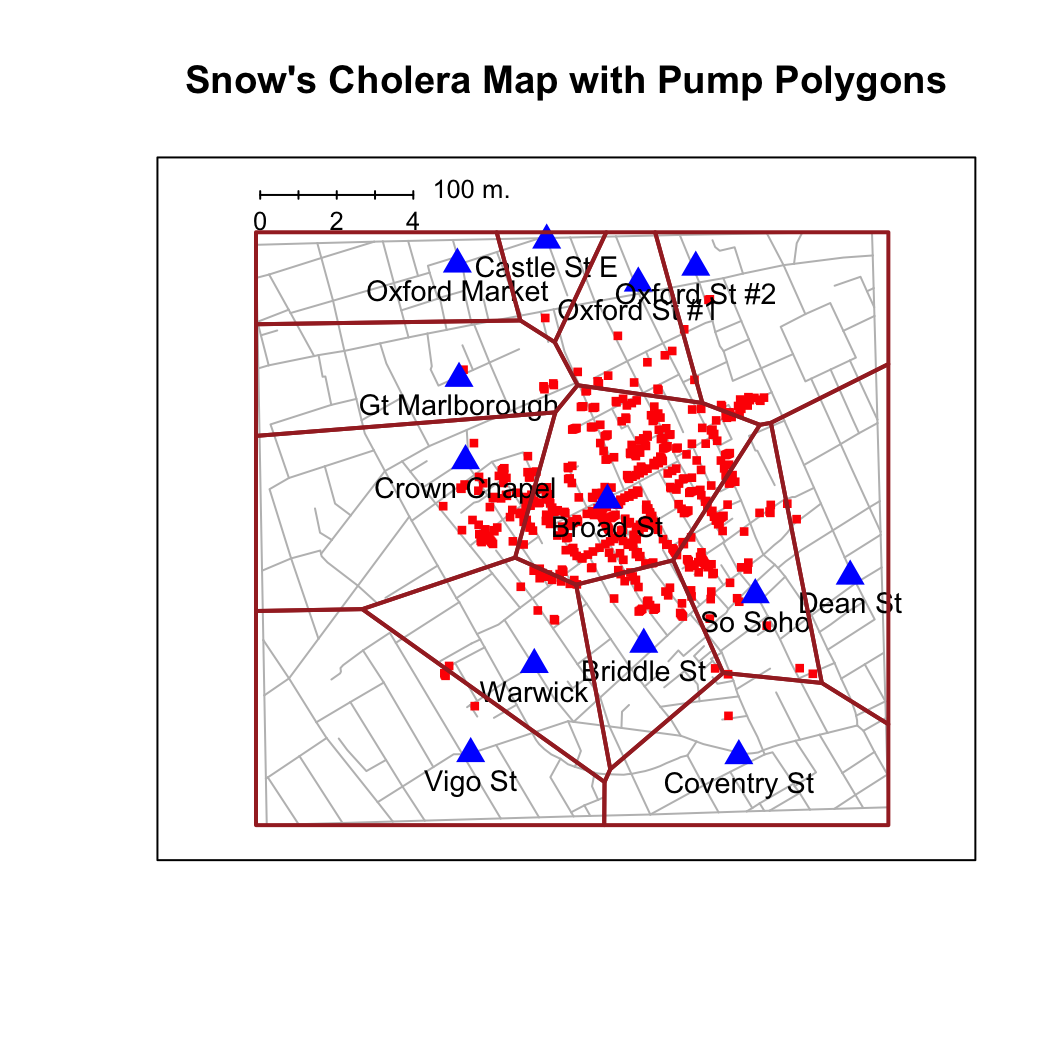
\includegraphics[width=0.6\linewidth]{06-notable_files/figure-latex/pump-1} \caption{Deaths (red dots) and pump locations.  Polygons that surround
each pump enclose the locations for which that is the nearest pump.}\label{fig:pump}
\end{figure}

Similar issues, arising from failures to ensure proper drainage systems,
were repeated, from the 1840s and 1850s through until~the end of the century,
in New Zealand cities. See\\
\href{https://teara.govt.nz/en/zoomify/24431/dunedin-renamed-stinkapool}{Christine Dann, Sewage, water and waste - Stinking cities', Te Ara - the Encyclopedia of New Zealand, (8 June 2017)}\footnote{\url{https://teara.govt.nz/en/zoomify/24431/dunedin-renamed-stinkapool}}

\hypertarget{the-reinhoff-and-rogoff-saga-smith-p.55}{%
\section{The Reinhoff and Rogoff saga (Smith, p.55)}\label{the-reinhoff-and-rogoff-saga-smith-p.55}}

Figure \ref{fig:debt2gdp12} plots data that underpinned
the 2010 paper ``\emph{Growth in Time of Debt}'' by the two Harvard economic
historians Reinhart and Rogoff {[}RR{]}. The paper \citep{reinhart2010growth}
has been widely quoted in support of economic austerity programs
internationally. There was a huge stir, in the media and on the
blogosphere, when graduate student Herndon found and published
details of coding and other errors in the results that RR had
presented.

\begin{verbatim}
## 
## Attaching package: 'nlme'
\end{verbatim}

\begin{verbatim}
## The following object is masked from 'package:HistData':
## 
##     Wheat
\end{verbatim}

\begin{verbatim}
## This is mgcv 1.8-34. For overview type 'help("mgcv-package")'.
\end{verbatim}

\begin{figure}[H]

{\centering 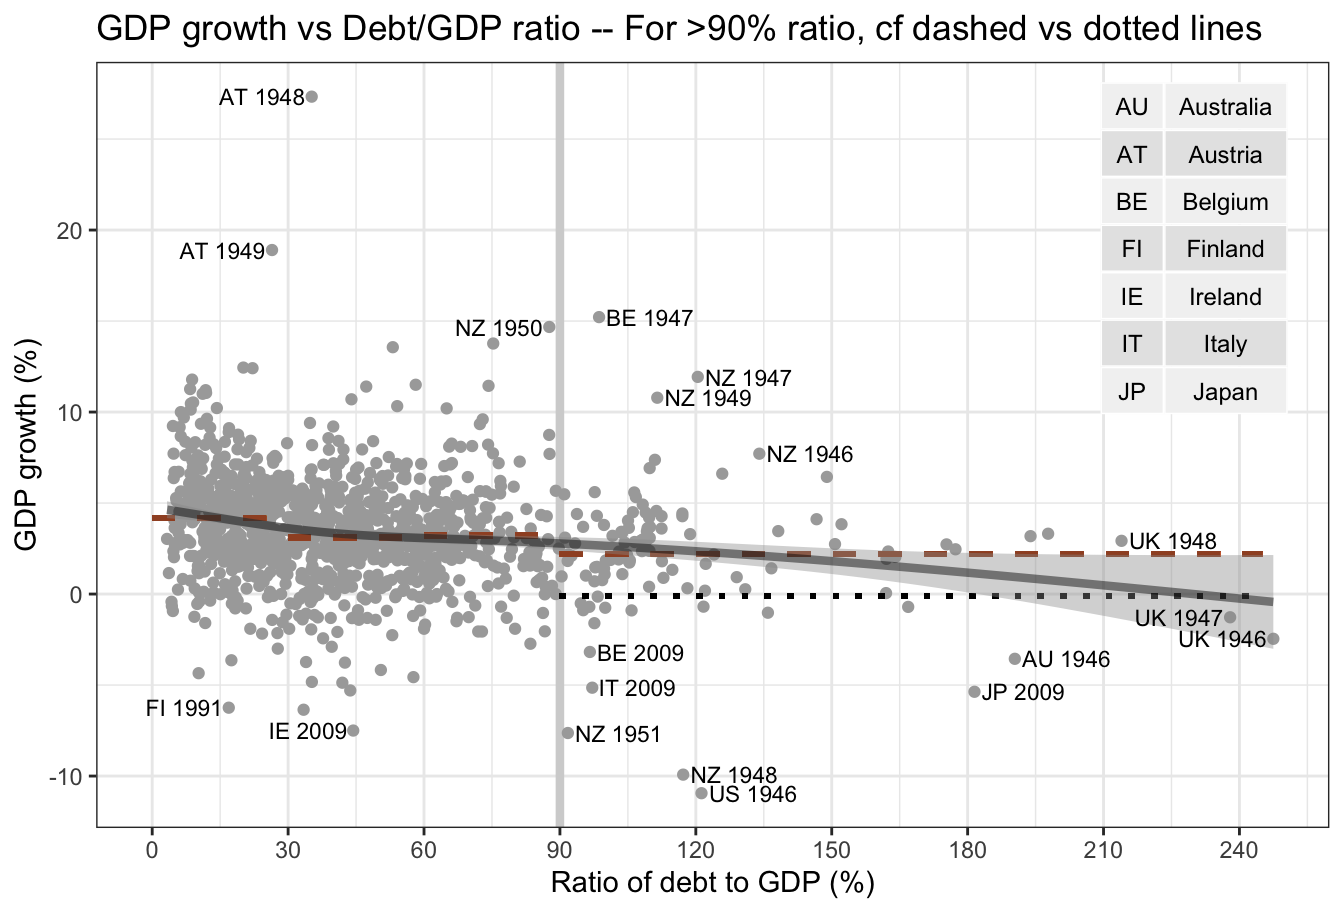
\includegraphics[width=1\linewidth]{06-notable_files/figure-latex/debt2gdp12-1} 

}

\caption{Red lines show means by Debt/GDP category.
The means for > 90\% Debt/GDP were from data for 10 only of the
20 countries.  The red dotted line shows the (incorrect) 
mean given by RR.  The smooth curve, fitted treating points
as independent, shows no sudden change.  It makes better sense
to allow each country its own separate curve.}\label{fig:debt2gdp12}
\end{figure}

As well as coding errors,
\href{http://www.peri.umass.edu/fileadmin/pdf/working_papers/working_papers_301-350/WP322.pdf}{Herndon}\footnote{\url{http://www.peri.umass.edu/fileadmin/pdf/working_papers/working_papers_301-350/WP322.pdf}} identified selective exclusion of available data,
and unconventional weighting of summary statistics. There was a
failure to acknowledge that the relationship studied has varied
substantially by country and over time.

In response to \citet{herndon2014does} and other critics, Reinhart and
Rogoff accepted that coding errors had led to the omission of
several countries, but pushed back against other criticisms.
Their revised analysis addresses only the most egregious errors
in their work. Among other issues, their insistence on treating
each data point for each country as an independent piece of
evidence makes no sense.

The smooth curve seems as good a summary as any, if
points are, wrongly, to be treated as disconnected from country.

\begin{figure}
\centering
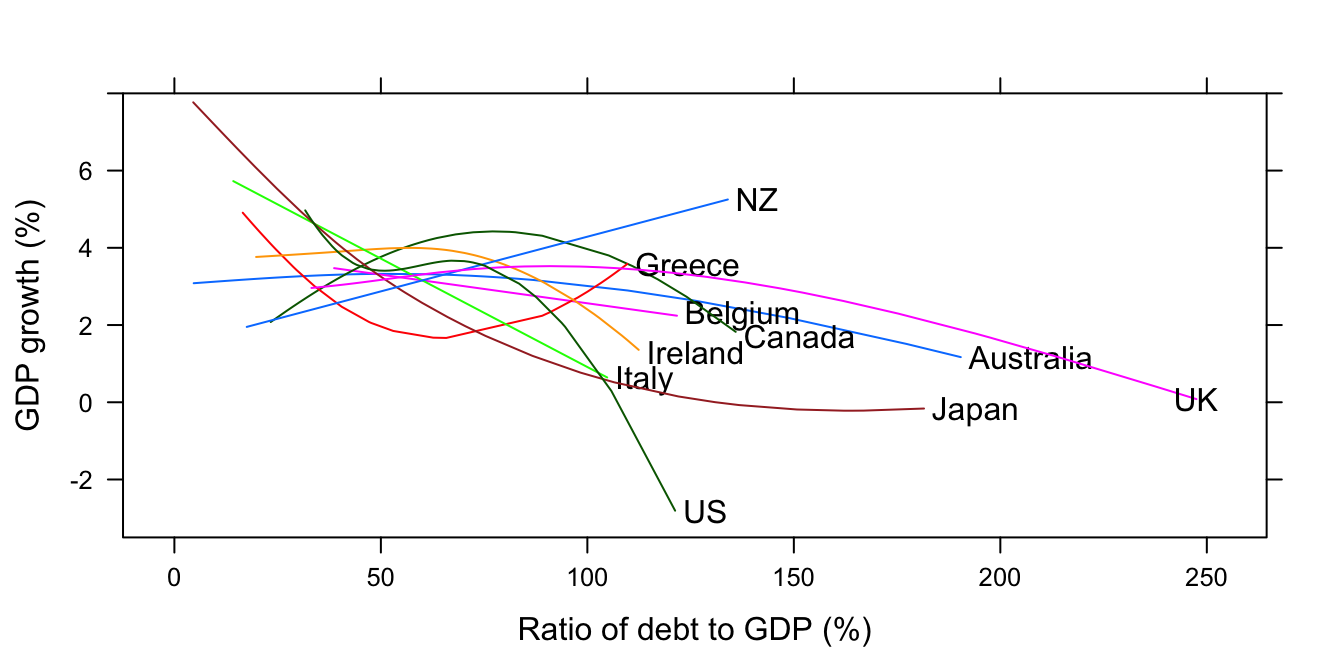
\includegraphics{06-notable_files/figure-latex/debt2gdp-3-1.pdf}
\caption{\label{fig:debt2gdp-3}Smooths have been fitted for each of the 10 countries
for which debt to GDP ratios were in some years greater than 90\%.
There is no consistent pattern, as there should be if RR's claim
is to hold up.}
\end{figure}

\hypertarget{is-there-a-pattern-across-countries}{%
\subsection*{Is there a pattern across countries?}\label{is-there-a-pattern-across-countries}}
\addcontentsline{toc}{subsection}{Is there a pattern across countries?}

\begin{Shaded}
\begin{Highlighting}[]
\NormalTok{av4 }\OtherTok{\textless{}{-}} \FunctionTok{sapply}\NormalTok{(}\FunctionTok{split}\NormalTok{(RR,RR}\SpecialCharTok{$}\NormalTok{Country), }\ControlFlowTok{function}\NormalTok{(x)}
\FunctionTok{c}\NormalTok{(}\AttributeTok{avTO30 =} \FunctionTok{mean}\NormalTok{(}\FunctionTok{subset}\NormalTok{(x, debtgdp}\SpecialCharTok{\textless{}=}\DecValTok{90}\NormalTok{)[ ,}\StringTok{\textquotesingle{}dRGDP\textquotesingle{}}\NormalTok{]),}
\AttributeTok{av30TO60 =} \FunctionTok{mean}\NormalTok{(}\FunctionTok{subset}\NormalTok{(x, debtgdp}\SpecialCharTok{\textgreater{}}\DecValTok{30} \SpecialCharTok{\&}\NormalTok{ debtgdp}\SpecialCharTok{\textless{}=}\DecValTok{60}\NormalTok{)[ ,}\StringTok{\textquotesingle{}dRGDP\textquotesingle{}}\NormalTok{]),}
\AttributeTok{av60TO90 =} \FunctionTok{mean}\NormalTok{(}\FunctionTok{subset}\NormalTok{(x, debtgdp}\SpecialCharTok{\textgreater{}}\DecValTok{60} \SpecialCharTok{\&}\NormalTok{ debtgdp}\SpecialCharTok{\textless{}=}\DecValTok{90}\NormalTok{)[ ,}\StringTok{\textquotesingle{}dRGDP\textquotesingle{}}\NormalTok{]),}
\AttributeTok{av90plus =} \FunctionTok{mean}\NormalTok{(}\FunctionTok{subset}\NormalTok{(x, debtgdp}\SpecialCharTok{\textgreater{}}\DecValTok{90}\NormalTok{)[ ,}\StringTok{\textquotesingle{}dRGDP\textquotesingle{}}\NormalTok{]),}
\AttributeTok{nyears =} \FunctionTok{nrow}\NormalTok{(}\FunctionTok{subset}\NormalTok{(x, debtgdp}\SpecialCharTok{\textgreater{}}\DecValTok{90}\NormalTok{))))}
\NormalTok{av4n }\OtherTok{\textless{}{-}}\NormalTok{ av4[,}\SpecialCharTok{!}\FunctionTok{is.nan}\NormalTok{(av4[}\DecValTok{4}\NormalTok{,])]}
\NormalTok{dRGDPav }\OtherTok{\textless{}{-}} \FunctionTok{sum}\NormalTok{(av4n[}\DecValTok{4}\NormalTok{,]}\SpecialCharTok{*}\NormalTok{av4n[}\DecValTok{5}\NormalTok{,])}\SpecialCharTok{/}\FunctionTok{sum}\NormalTok{(av4[}\DecValTok{5}\NormalTok{,])}
\end{Highlighting}
\end{Shaded}

There were just 10 countries where debt to GDP ratios were
greater than 90\% for one or more years. For 9 of
those countries, the average of their GDP growth in the years at issue
was on average positive relative to the previous year. The average
percentage growth over all 10 countries, weighted according
to number of years, was 2.168.

\hypertarget{there-are-further-serious-issues-of-interpretation}{%
\section*{There are further serious issues of interpretation}\label{there-are-further-serious-issues-of-interpretation}}
\addcontentsline{toc}{section}{There are further serious issues of interpretation}

\begin{itemize}
\tightlist
\item
  Does GDP drive debt/GDP ratio, or is it the other way round?

  \begin{itemize}
  \tightlist
  \item
    Or does a third factor drive both?
  \end{itemize}
\item
  Is the effect immediate, or on future economic performance
\end{itemize}

Smith (p.64) refers to work indicating that economic performance
is more closely correlated with economic growth in the past than
with future growth.

\hypertarget{parting-comments}{%
\section*{Parting comments}\label{parting-comments}}
\addcontentsline{toc}{section}{Parting comments}

\citet{herndon2014does} comment

``\ldots{} RR's findings have served as an intellectual bulwark in support of austerity politics. The fact that RR's findings are wrong should therefore lead us to reassess the austerity agenda itself in both Europe and the United States.''

The saga emphasizes the importance of working with reproducible code,
rather than with spreadsheet calculations.
The errors in RR's calculations were from one perspective fortunate.
Once highlighted, the errors drew critical attention to the paper,
and to the serious flaws in the analysis.

\hypertarget{sec:yule1}{%
\chapter{Weighting effects, \& the Yule-Simpson Paradox}\label{sec:yule1}}

\hypertarget{deaths-from-covid-19-between-country-comparisons}{%
\section{Deaths from Covid-19 --- between country comparisons}\label{deaths-from-covid-19-between-country-comparisons}}

United States data for the 13 months up to 31 January 2021 shows
a stark difference in death rates, for those in younger as
compared with those in older age groups, as shown in Figure
\ref{fig:riskByAge}.

\begin{Shaded}
\begin{Highlighting}[]
\NormalTok{cap\_props }\OtherTok{\textless{}{-}} \FunctionTok{paste0}\NormalTok{(}\StringTok{"United States reported deaths per 100 from Covid{-}19}
\StringTok{(and, for comparison, deaths per 100), for the time period from "}\NormalTok{,}
\NormalTok{wkStartEnd[}\DecValTok{1}\NormalTok{], }\StringTok{" to "}\NormalTok{, wkStartEnd[}\DecValTok{2}\NormalTok{], }\StringTok{". The total number}
\StringTok{reported was "}\NormalTok{, }\FunctionTok{sum}\NormalTok{(USdeadpop1yr}\SpecialCharTok{$}\NormalTok{covdeaths),}\StringTok{"."}\NormalTok{)}
\NormalTok{fromTo }\OtherTok{\textless{}{-}} \FunctionTok{format}\NormalTok{(UScausesByCats[}\DecValTok{1}\NormalTok{,}\DecValTok{2}\SpecialCharTok{:}\DecValTok{3}\NormalTok{],}\StringTok{"\%b \%d \%Y"}\NormalTok{)}
\end{Highlighting}
\end{Shaded}

\begin{figure}
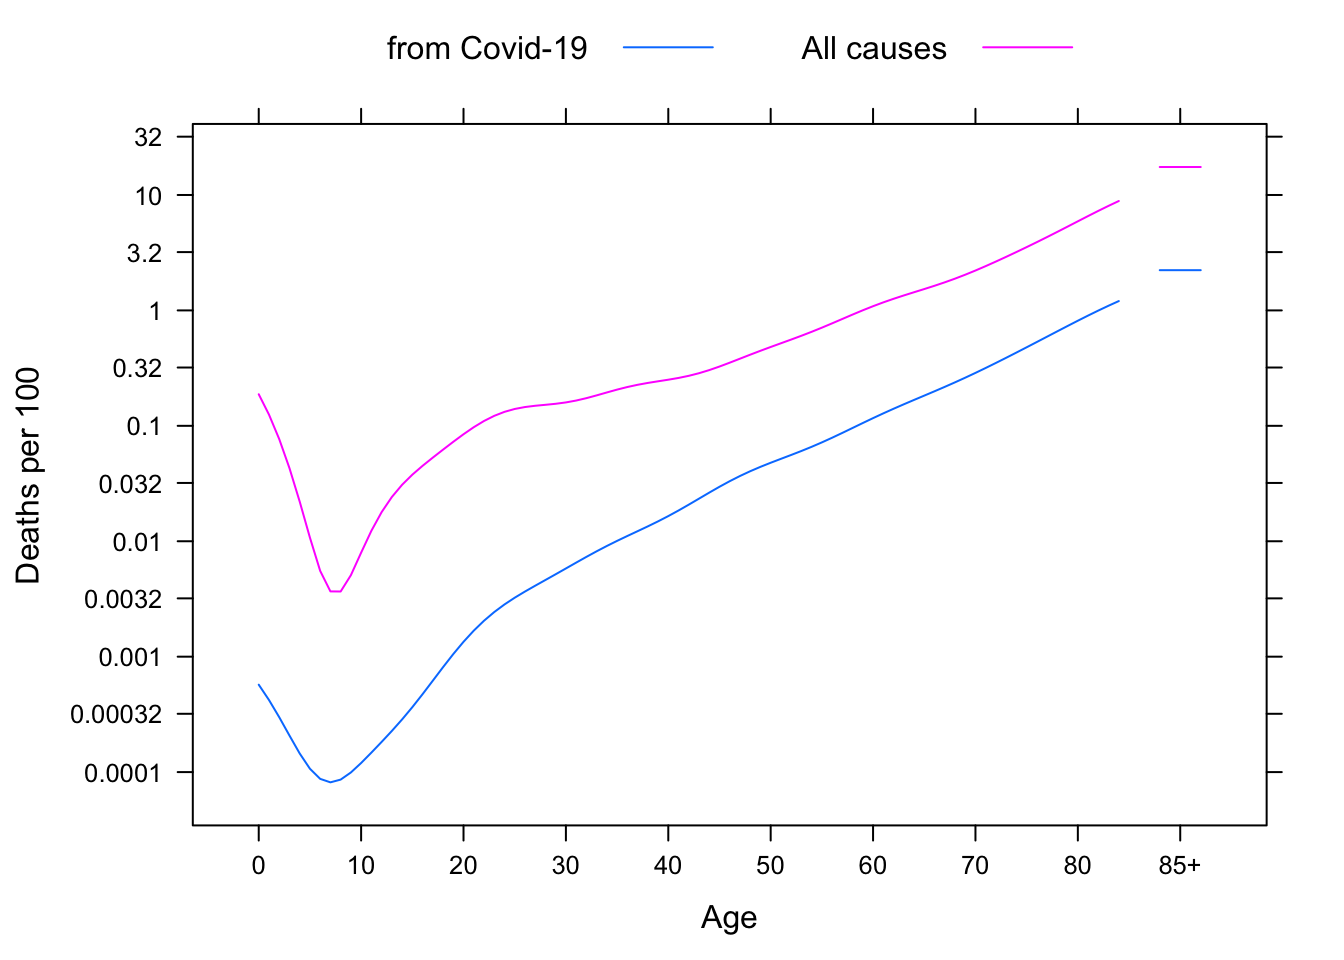
\includegraphics[width=0.5\linewidth]{07-weighting_files/figure-latex/riskByAge-1} \caption{Proportions who died, from Covid-19, and in total}\label{fig:riskByAge}
\end{figure}

It is immediately obvious that more deaths are to expected, assuming a similar
breakdown by age, in countries where there are more old people. Thus, the
death rates per 1000 for Covid-19, for under age 65 as opposed to age \(>=\) 65,
were:

\begin{verbatim}
##  <65 >=65 
## 0.28 6.30
\end{verbatim}

Now observe how these rates transfer across to countries with a different population
structure.

\begin{verbatim}
##                                US Italy Kenya
## Percentage 65 or more        16.3  23.3   2.5
## Expected deaths per 100,000 126.7 168.5  43.5
## Reported deaths per 100,000 126.7 146.0   3.3
\end{verbatim}

Italy has a higher proportion of older people, leading to a higher
expected death-rate. Kenya has a much lower proportion, and a lower
expected overall death-rate. Other totals, e.g., for infection rates
or hospital admissions, while still impacted by age structure, were not
impacted to the same extent. A table on the US Center for Disease
Control web page {[}Hospitalization and Death by Age{]} (\url{https://www.cdc.gov/coronavirus/2019-ncov/covid-data/investigations-discovery/hospitalization-death-by-age.html})
shows how, in the US, hospitalization and death varied with
age. Whereas death rates for those 85 years of age or older were
810 times those of 5-17 year olds, for hospitalization the multiplier
was 52. The rates for 0-4 year olds were around twice those for
5-17 year olds. Overall rates varied, in both cases, with ethnicity.

Between country comparisons can be hazardous. There are likely to be
differences in the completeness of the data and in recording protocols.
Case numbers are likely to be influenced by testing rates, are to be
substantial undercounts, to an extent that varies from country to country.

\hypertarget{the-yule-simpson-paradox-ucb-admissions-data}{%
\section{The Yule-Simpson paradox --- UCB admissions data}\label{the-yule-simpson-paradox-ucb-admissions-data}}

The Yule-Simpson paradox is a paradox of human intuition.
It arises when weighting effects operate with respect to two
or more factors. University of California Berkeley (UCB)
1973 admissions data for the six largest departments,
summarized in Figure \ref{fig:UCBgph1}, provides an example.
Admission rates varied by department, as did the relative
numbers of males and females applying, in ways that led to the
paradox. Male/female differences within departments were of
lesser consequence.

Overall admission rates across the six largest departments were:

\begin{Shaded}
\begin{Highlighting}[]
\DocumentationTok{\#\# Tabulate by Admit and Gender}
\NormalTok{byGender }\OtherTok{\textless{}{-}} \FunctionTok{margin.table}\NormalTok{(UCBAdmissions, }\AttributeTok{margin=}\DecValTok{1}\SpecialCharTok{:}\DecValTok{2}\NormalTok{)}
\FunctionTok{round}\NormalTok{(}\DecValTok{100}\SpecialCharTok{*}\FunctionTok{prop.table}\NormalTok{(byGender, }\AttributeTok{margin=}\DecValTok{2}\NormalTok{)[}\StringTok{"Admitted"}\NormalTok{, ], }\DecValTok{1}\NormalTok{)}
\end{Highlighting}
\end{Shaded}

\begin{verbatim}
##   Male Female 
##   44.5   30.4
\end{verbatim}

Taken at face value, these numbers suggest discrimination
against females,

\begin{Shaded}
\begin{Highlighting}[]
\FunctionTok{par}\NormalTok{(}\AttributeTok{mar=}\FunctionTok{c}\NormalTok{(}\FloatTok{3.1}\NormalTok{,}\FloatTok{3.1}\NormalTok{,}\FloatTok{2.6}\NormalTok{,}\FloatTok{0.6}\NormalTok{), }\AttributeTok{mgp=}\FunctionTok{c}\NormalTok{(}\DecValTok{2}\NormalTok{,}\FloatTok{0.5}\NormalTok{,}\DecValTok{0}\NormalTok{))}
\NormalTok{applied }\OtherTok{\textless{}{-}} \FunctionTok{margin.table}\NormalTok{(UCBAdmissions, }\AttributeTok{margin=}\DecValTok{2}\SpecialCharTok{:}\DecValTok{3}\NormalTok{)}
\NormalTok{pcAdmit }\OtherTok{\textless{}{-}} \DecValTok{100}\SpecialCharTok{*}\FunctionTok{prop.table}\NormalTok{(UCBAdmissions, }\AttributeTok{margin=}\DecValTok{2}\SpecialCharTok{:}\DecValTok{3}\NormalTok{)[}\StringTok{"Admitted"}\NormalTok{, , ]}
\NormalTok{byGender }\OtherTok{\textless{}{-}} \DecValTok{100}\SpecialCharTok{*}\FunctionTok{prop.table}\NormalTok{(}\FunctionTok{margin.table}\NormalTok{(UCBAdmissions,}
                                        \AttributeTok{margin=}\DecValTok{1}\SpecialCharTok{:}\DecValTok{2}\NormalTok{), }\AttributeTok{margin=}\DecValTok{2}\NormalTok{)}
\NormalTok{dimnam }\OtherTok{\textless{}{-}} \FunctionTok{dimnames}\NormalTok{(UCBAdmissions)}
\NormalTok{mfStats }\OtherTok{\textless{}{-}} \FunctionTok{data.frame}\NormalTok{(}\AttributeTok{Admit=}\FunctionTok{c}\NormalTok{(pcAdmit[}\DecValTok{1}\NormalTok{,],pcAdmit[}\DecValTok{2}\NormalTok{,]),}
                      \AttributeTok{Applicants=}\FunctionTok{c}\NormalTok{(applied[}\DecValTok{1}\NormalTok{,], applied[}\DecValTok{2}\NormalTok{,]),}
                      \AttributeTok{mf=}\FunctionTok{factor}\NormalTok{(}\FunctionTok{rep}\NormalTok{(dimnam[[}\StringTok{\textquotesingle{}Gender\textquotesingle{}}\NormalTok{]],}\FunctionTok{c}\NormalTok{(}\DecValTok{6}\NormalTok{,}\DecValTok{6}\NormalTok{)),}
                                \AttributeTok{levels=}\NormalTok{dimnam[[}\StringTok{\textquotesingle{}Gender\textquotesingle{}}\NormalTok{]]),}
                      \AttributeTok{Department=}\FunctionTok{rep}\NormalTok{(dimnam[[}\StringTok{"Dept"}\NormalTok{]],}\DecValTok{2}\NormalTok{))}
\NormalTok{xlim }\OtherTok{\textless{}{-}} \FunctionTok{c}\NormalTok{(}\DecValTok{0}\NormalTok{, }\FunctionTok{max}\NormalTok{(mfStats}\SpecialCharTok{$}\NormalTok{Admit)}\SpecialCharTok{*}\FloatTok{1.025}\NormalTok{)}
\NormalTok{ylim }\OtherTok{\textless{}{-}} \FunctionTok{c}\NormalTok{(}\DecValTok{0}\NormalTok{, }\FunctionTok{max}\NormalTok{(mfStats}\SpecialCharTok{$}\NormalTok{Applicants)}\SpecialCharTok{*}\FloatTok{1.075}\NormalTok{)}
\FunctionTok{plot}\NormalTok{(Applicants}\SpecialCharTok{\textasciitilde{}}\NormalTok{Admit, }\AttributeTok{data=}\NormalTok{mfStats, }\AttributeTok{xlim=}\NormalTok{xlim, }\AttributeTok{ylim=}\NormalTok{ylim,}
     \AttributeTok{fg=}\StringTok{"gray"}\NormalTok{, }\AttributeTok{cex.lab=}\FloatTok{1.25}\NormalTok{,}
     \AttributeTok{col=}\FunctionTok{rep}\NormalTok{(}\FunctionTok{c}\NormalTok{(}\StringTok{"blue"}\NormalTok{,}\StringTok{"red"}\NormalTok{),}\FunctionTok{rep}\NormalTok{(}\DecValTok{6}\NormalTok{,}\DecValTok{2}\NormalTok{)),}\AttributeTok{type=}\StringTok{"h"}\NormalTok{,}\AttributeTok{lwd=}\DecValTok{2}\NormalTok{,}
     \AttributeTok{xlab=}\StringTok{"UCB Admission rates (\%), 1973"}\NormalTok{, }
     \AttributeTok{ylab=}\StringTok{"Number of applicants"}\NormalTok{)}
\NormalTok{pcA }\OtherTok{\textless{}{-}} \FunctionTok{rbind}\NormalTok{(pcAdmit[}\DecValTok{1}\NormalTok{,], }\FunctionTok{apply}\NormalTok{(pcAdmit,}\DecValTok{2}\NormalTok{, mean)}\SpecialCharTok{+}\DecValTok{2}\NormalTok{, pcAdmit[}\DecValTok{2}\NormalTok{,], }\FunctionTok{rep}\NormalTok{(}\ConstantTok{NA}\NormalTok{,}\DecValTok{6}\NormalTok{))}
\NormalTok{pcA[}\DecValTok{2}\NormalTok{,}\DecValTok{3}\NormalTok{] }\OtherTok{\textless{}{-}}\NormalTok{ pcA[}\DecValTok{2}\NormalTok{,}\DecValTok{3}\NormalTok{]}\SpecialCharTok{+}\DecValTok{1}
\NormalTok{appA }\OtherTok{\textless{}{-}} \FunctionTok{rbind}\NormalTok{(applied[}\DecValTok{1}\NormalTok{,], }\FunctionTok{apply}\NormalTok{(applied,}\DecValTok{2}\NormalTok{, mean)}\SpecialCharTok{+}\DecValTok{80}\NormalTok{,}
\NormalTok{              applied[}\DecValTok{2}\NormalTok{,], }\FunctionTok{rep}\NormalTok{(}\ConstantTok{NA}\NormalTok{,}\DecValTok{6}\NormalTok{))}
\NormalTok{deptNam }\OtherTok{\textless{}{-}}\NormalTok{ dimnam[[}\DecValTok{3}\NormalTok{]]}
\ControlFlowTok{for}\NormalTok{(j }\ControlFlowTok{in} \DecValTok{1}\SpecialCharTok{:}\FunctionTok{ncol}\NormalTok{(appA))}
  \FunctionTok{lines}\NormalTok{(pcA[,j], appA[,j], }\AttributeTok{type=}\StringTok{"c"}\NormalTok{, }\AttributeTok{col=}\StringTok{"gray"}\NormalTok{)}
\FunctionTok{text}\NormalTok{(pcA[}\DecValTok{2}\NormalTok{,],appA[}\DecValTok{2}\NormalTok{,],deptNam)}
\DocumentationTok{\#\#}
\FunctionTok{par}\NormalTok{(}\AttributeTok{xpd=}\ConstantTok{TRUE}\NormalTok{)}
\FunctionTok{text}\NormalTok{(byGender[}\DecValTok{1}\NormalTok{,}\DecValTok{1}\SpecialCharTok{:}\DecValTok{2}\NormalTok{], }\FunctionTok{rep}\NormalTok{(}\FunctionTok{par}\NormalTok{()}\SpecialCharTok{$}\NormalTok{usr[}\DecValTok{4}\NormalTok{],}\DecValTok{2}\NormalTok{)}\SpecialCharTok{+}\FloatTok{0.5}\SpecialCharTok{*}\FunctionTok{strheight}\NormalTok{(}\StringTok{"\^{}"}\NormalTok{), }\AttributeTok{labels=}\FunctionTok{c}\NormalTok{(}\StringTok{"\^{}"}\NormalTok{,}\StringTok{"\^{}"}\NormalTok{),}
     \AttributeTok{col=}\FunctionTok{c}\NormalTok{(}\StringTok{"blue"}\NormalTok{,}\StringTok{"red"}\NormalTok{),}\AttributeTok{cex=}\FloatTok{1.25}\NormalTok{,}\AttributeTok{srt=}\DecValTok{180}\NormalTok{)}
\FunctionTok{text}\NormalTok{(byGender[}\DecValTok{1}\NormalTok{,], }\FunctionTok{par}\NormalTok{()}\SpecialCharTok{$}\NormalTok{usr[}\DecValTok{4}\NormalTok{]}\SpecialCharTok{+}\FloatTok{1.4}\SpecialCharTok{*}\FunctionTok{strheight}\NormalTok{(}\StringTok{"A"}\NormalTok{),}
     \AttributeTok{labels=}\FunctionTok{paste}\NormalTok{(}\FunctionTok{round}\NormalTok{(byGender[}\DecValTok{1}\NormalTok{,],}\DecValTok{1}\NormalTok{)),}\AttributeTok{cex=}\FloatTok{0.85}\NormalTok{)}
\FunctionTok{text}\NormalTok{(byGender[}\DecValTok{1}\NormalTok{,}\DecValTok{1}\SpecialCharTok{:}\DecValTok{2}\NormalTok{]}\SpecialCharTok{+}\FunctionTok{c}\NormalTok{(}\SpecialCharTok{{-}}\FloatTok{3.5}\NormalTok{,}\FloatTok{3.5}\NormalTok{), }\FunctionTok{rep}\NormalTok{(}\FunctionTok{par}\NormalTok{()}\SpecialCharTok{$}\NormalTok{usr[}\DecValTok{4}\NormalTok{],}\DecValTok{2}\NormalTok{)}\SpecialCharTok{+}\FloatTok{2.65}\SpecialCharTok{*}\FunctionTok{strheight}\NormalTok{(}\StringTok{"A"}\NormalTok{),}
     \AttributeTok{labels=}\FunctionTok{c}\NormalTok{(}\StringTok{"All males"}\NormalTok{,}\StringTok{"All females"}\NormalTok{), }\AttributeTok{pos=}\FunctionTok{c}\NormalTok{(}\DecValTok{4}\NormalTok{,}\DecValTok{2}\NormalTok{), }\AttributeTok{cex=}\FloatTok{1.25}\NormalTok{)}
\FunctionTok{par}\NormalTok{(}\AttributeTok{xpd=}\ConstantTok{FALSE}\NormalTok{)}
\FunctionTok{abline}\NormalTok{(}\AttributeTok{h=}\DecValTok{200}\SpecialCharTok{*}\NormalTok{(}\DecValTok{0}\SpecialCharTok{:}\DecValTok{4}\NormalTok{),}\AttributeTok{col=}\StringTok{"lightgray"}\NormalTok{,}\AttributeTok{lty=}\StringTok{"dotted"}\NormalTok{)}
\FunctionTok{abline}\NormalTok{(}\AttributeTok{v=}\DecValTok{20}\SpecialCharTok{*}\NormalTok{(}\DecValTok{0}\SpecialCharTok{:}\DecValTok{4}\NormalTok{),}\AttributeTok{col=}\StringTok{"lightgray"}\NormalTok{,}\AttributeTok{lty=}\StringTok{"dotted"}\NormalTok{)}
\FunctionTok{legend}\NormalTok{(}\StringTok{"topleft"}\NormalTok{, }\AttributeTok{col=}\FunctionTok{c}\NormalTok{(}\StringTok{\textquotesingle{}blue\textquotesingle{}}\NormalTok{,}\StringTok{\textquotesingle{}red\textquotesingle{}}\NormalTok{),}\AttributeTok{lty=}\FunctionTok{c}\NormalTok{(}\DecValTok{1}\NormalTok{,}\DecValTok{1}\NormalTok{), }\AttributeTok{lwd=}\FloatTok{0.75}\NormalTok{, }\AttributeTok{cex=}\FloatTok{0.9}\NormalTok{,}
       \AttributeTok{y.intersp=}\FloatTok{0.65}\NormalTok{, }\AttributeTok{legend=}\FunctionTok{c}\NormalTok{(}\StringTok{"Males"}\NormalTok{,}\StringTok{"Females"}\NormalTok{),}\AttributeTok{bty=}\StringTok{"n"}\NormalTok{)}
\end{Highlighting}
\end{Shaded}

\begin{figure}[H]
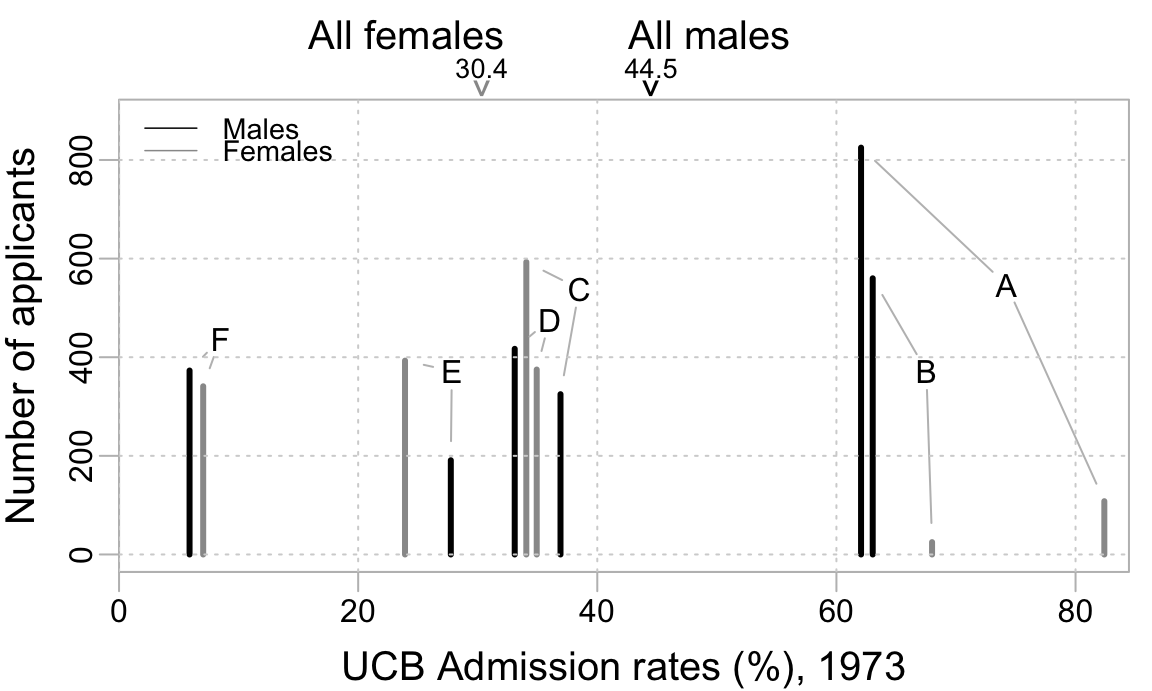
\includegraphics[width=0.72\linewidth]{07-weighting_files/figure-latex/UCBgph1-1} \caption{UCB admossion data for 1973, accounting for male/female differences, by department.  Department labels range from A to E.}\label{fig:UCBgph1}
\end{figure}

Admission rates for males and females, by department, tell a different
story:

\begin{Shaded}
\begin{Highlighting}[]
\NormalTok{admit }\OtherTok{\textless{}{-}} \FunctionTok{round}\NormalTok{(}\DecValTok{100}\SpecialCharTok{*}\FunctionTok{prop.table}\NormalTok{(UCBAdmissions,}
                     \AttributeTok{margin=}\DecValTok{2}\SpecialCharTok{:}\DecValTok{3}\NormalTok{)[}\StringTok{"Admitted"}\NormalTok{, , ], }\DecValTok{1}\NormalTok{)}
\NormalTok{tab }\OtherTok{\textless{}{-}}\NormalTok{ xtable}\SpecialCharTok{::}\FunctionTok{xtable}\NormalTok{(admit, }\AttributeTok{digits=}\DecValTok{1}\NormalTok{)}
\FunctionTok{print}\NormalTok{(tab, }\AttributeTok{type=}\StringTok{\textquotesingle{}latex\textquotesingle{}}\NormalTok{, }\AttributeTok{comment=}\ConstantTok{FALSE}\NormalTok{, }\AttributeTok{floating=}\ConstantTok{FALSE}\NormalTok{, }\AttributeTok{scalebox=}\FloatTok{0.9}\NormalTok{)}
\end{Highlighting}
\end{Shaded}

\scalebox{0.9}{
\begin{tabular}{rrrrrrr}
  \hline
 & A & B & C & D & E & F \\ 
  \hline
Male & 62.1 & 63.0 & 36.9 & 33.1 & 27.7 & 5.9 \\ 
  Female & 82.4 & 68.0 & 34.1 & 34.9 & 23.9 & 7.0 \\ 
   \hline
\end{tabular}
}

The biggest differences in admission rates were in departments
A (82.4\%-62.1\%=20.3\%) and B (68\%-63\%=5\%), in both cases favouring females.
In the other four departments, differences were 3.8\% or less.

In order to understand how this happens, it is necessary to look
at how the numbers that applied break down by gender and by department:

\begin{Shaded}
\begin{Highlighting}[]
\FunctionTok{library}\NormalTok{(xtable)}
\NormalTok{tots }\OtherTok{\textless{}{-}} \FunctionTok{margin.table}\NormalTok{(UCBAdmissions, }\AttributeTok{margin=}\DecValTok{2}\SpecialCharTok{:}\DecValTok{3}\NormalTok{)}
\NormalTok{tab }\OtherTok{\textless{}{-}}\NormalTok{ xtable}\SpecialCharTok{::}\FunctionTok{xtable}\NormalTok{(tots, }\AttributeTok{digits=}\DecValTok{0}\NormalTok{)}
\FunctionTok{print}\NormalTok{(tab,}\AttributeTok{type=}\StringTok{\textquotesingle{}latex\textquotesingle{}}\NormalTok{, }\AttributeTok{comment=}\ConstantTok{FALSE}\NormalTok{, }\AttributeTok{floating=}\ConstantTok{FALSE}\NormalTok{, }\AttributeTok{scalebox=}\FloatTok{0.9}\NormalTok{)}
\end{Highlighting}
\end{Shaded}

\scalebox{0.9}{
\begin{tabular}{rrrrrrr}
  \hline
 & A & B & C & D & E & F \\ 
  \hline
Male & 825 & 560 & 325 & 417 & 191 & 373 \\ 
  Female & 108 & 25 & 593 & 375 & 393 & 341 \\ 
   \hline
\end{tabular}
}

Comparing departments A and B with other departments, one finds:

\begin{verbatim}
##         
##                       AB                CDEF
##   Male   1385 (62.1,63%)  981 (5.9 to 36.9%)
##   Female  133 (82.4,68%) 1109 (7.0 to 34.9%)
\end{verbatim}

\begin{itemize}
\tightlist
\item
  Overall admission rates for males are weighted (1385:981) towards
  male rates of 62.1\% or 63\% in departments A and B.
\item
  Those for females are strongly weighted (1109:133) towards admission rates that range from 5.9\% to 34.1\% in departments C to F.
\end{itemize}

\hypertarget{ucb-admissions-data-another-perspective}{%
\subsection*{UCB Admissions Data -- Another perspective}\label{ucb-admissions-data-another-perspective}}
\addcontentsline{toc}{subsection}{UCB Admissions Data -- Another perspective}

\begin{Shaded}
\begin{Highlighting}[]
\FunctionTok{par}\NormalTok{(}\AttributeTok{mar=}\FunctionTok{c}\NormalTok{(}\FloatTok{3.1}\NormalTok{,}\FloatTok{3.1}\NormalTok{,}\FloatTok{2.1}\NormalTok{,}\FloatTok{0.6}\NormalTok{), }\AttributeTok{mgp=}\FunctionTok{c}\NormalTok{(}\DecValTok{2}\NormalTok{,}\FloatTok{0.5}\NormalTok{,}\DecValTok{0}\NormalTok{))}
\NormalTok{diffAdmit }\OtherTok{\textless{}{-}} \FunctionTok{t}\NormalTok{(pcAdmit)}
\NormalTok{diffAdmit }\OtherTok{\textless{}{-}} \FunctionTok{data.frame}\NormalTok{(}\AttributeTok{dept=}\FunctionTok{rownames}\NormalTok{(diffAdmit), }\AttributeTok{stringsAsFactors=}\ConstantTok{FALSE}\NormalTok{,}
                        \AttributeTok{Male=}\NormalTok{diffAdmit[,}\DecValTok{1}\NormalTok{],}\AttributeTok{Female=}\NormalTok{diffAdmit[,}\DecValTok{2}\NormalTok{],}
                        \AttributeTok{diff=}\NormalTok{diffAdmit[,}\DecValTok{2}\NormalTok{]}\SpecialCharTok{{-}}\NormalTok{diffAdmit[,}\DecValTok{1}\NormalTok{])}
\NormalTok{diffAdmit}\SpecialCharTok{$}\NormalTok{mfratio }\OtherTok{\textless{}{-}} \FunctionTok{signif}\NormalTok{(}\FunctionTok{apply}\NormalTok{(applied,}\DecValTok{2}\NormalTok{, }\ControlFlowTok{function}\NormalTok{(x)x[}\DecValTok{1}\NormalTok{]}\SpecialCharTok{/}\NormalTok{x[}\DecValTok{2}\NormalTok{]),}\DecValTok{2}\NormalTok{)}
\NormalTok{ord }\OtherTok{\textless{}{-}} \FunctionTok{order}\NormalTok{(diffAdmit}\SpecialCharTok{$}\NormalTok{diff)}
\FunctionTok{plot}\NormalTok{(diff }\SpecialCharTok{\textasciitilde{}} \FunctionTok{I}\NormalTok{(}\DecValTok{1}\SpecialCharTok{:}\DecValTok{6}\NormalTok{), }\AttributeTok{data=}\NormalTok{diffAdmit[ord,], }\AttributeTok{pch=}\NormalTok{dept, }\AttributeTok{cex=}\FloatTok{1.25}\NormalTok{,}
     \AttributeTok{ylim=}\FunctionTok{c}\NormalTok{(}\SpecialCharTok{{-}}\FloatTok{5.25}\NormalTok{,}\FloatTok{21.5}\NormalTok{), }\AttributeTok{xlab=}\StringTok{"Order of difference"}\NormalTok{, }\AttributeTok{fg=}\StringTok{"gray"}\NormalTok{,}
     \AttributeTok{ylab=}\StringTok{"Female {-} Male difference (\%)"}\NormalTok{)}
\FunctionTok{with}\NormalTok{(diffAdmit[ord,], }\FunctionTok{text}\NormalTok{(diff}\SpecialCharTok{\textasciitilde{}}\FunctionTok{I}\NormalTok{(}\DecValTok{1}\SpecialCharTok{:}\DecValTok{6}\NormalTok{), }\AttributeTok{labels=}\FunctionTok{paste}\NormalTok{(mfratio), }
                           \AttributeTok{pos=}\FunctionTok{c}\NormalTok{(}\FunctionTok{rep}\NormalTok{(}\DecValTok{4}\NormalTok{,}\DecValTok{5}\NormalTok{),}\DecValTok{2}\NormalTok{)), }\AttributeTok{cex=}\FloatTok{0.8}\NormalTok{)}
\NormalTok{leg }\OtherTok{\textless{}{-}} \FunctionTok{c}\NormalTok{(}\StringTok{"Male:Female ratios of numbers"}\NormalTok{,}
         \StringTok{"who applied are shown alongside"}\NormalTok{,}
         \StringTok{"each letter"}\NormalTok{)}
\FunctionTok{legend}\NormalTok{(}\StringTok{"topleft"}\NormalTok{, }\AttributeTok{legend=}\NormalTok{leg, }\AttributeTok{box.col=}\StringTok{"gray"}\NormalTok{)}
\end{Highlighting}
\end{Shaded}

\begin{figure}[H]
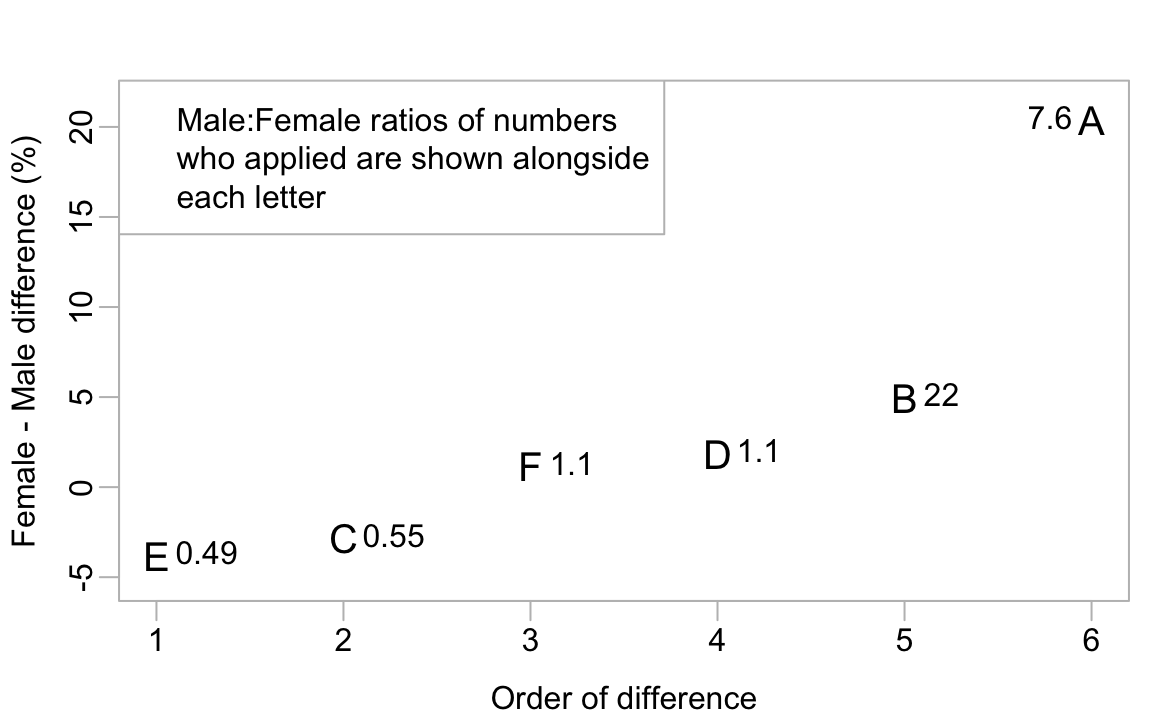
\includegraphics[width=0.72\linewidth]{07-weighting_files/figure-latex/UCBdiffs-1} \caption{UCB admossion data for 1973 --- another perspective.}\label{fig:UCBdiffs}
\end{figure}

Effective graphs can help greatly in fairly representing the evidence.
The website
\url{https://www.youtube.com/watch?v=ZDinnCwP3dg}
has an animated video that provides a short overview of the paradox.

The same sorts of paradoxical effects can be found in regression.
The Yule-Simpson paradox may be regarded as a special case of Lord's
paradox, described in \citet{lord1967paradox}. Any attempt to attach meaning
to regression coefficients can be highly misleading, unless one can be
sure that effects of all variates and covariates are properly
accounted for. It is rarely easy, with observational data, to be sure
that this has been done effectively.

\hypertarget{third-variables-change-the-story-further-examples}{%
\section{Third variables change the story --- further examples}\label{third-variables-change-the-story-further-examples}}

Here, ``variable'' is used as generic name for either continuous
variables, or categorical variables, otherwise called factors.

\hypertarget{does-baclofen-help-in-reducing-pain}{%
\subsection*{Does Baclofen help in reducing pain?}\label{does-baclofen-help-in-reducing-pain}}
\addcontentsline{toc}{subsection}{Does Baclofen help in reducing pain?}

\begin{Shaded}
\begin{Highlighting}[]
\NormalTok{cap9 }\OtherTok{\textless{}{-}} \StringTok{"Data are pain reduction scores. Subgroup numbers, shown}
\StringTok{    below each point, weight the overall average (\textquotesingle{}\textquotesingle{}ALL\textquotesingle{}\textquotesingle{}) for}
\StringTok{    baclofen towards the high female average, and for no baclofen}
\StringTok{    slightly towards the low male average."}
\end{Highlighting}
\end{Shaded}

\begin{Shaded}
\begin{Highlighting}[]
\FunctionTok{library}\NormalTok{(lattice)}
\NormalTok{parset }\OtherTok{\textless{}{-}} \FunctionTok{simpleTheme}\NormalTok{(}\AttributeTok{cex=}\FloatTok{1.35}\NormalTok{, }\AttributeTok{pch=}\DecValTok{16}\NormalTok{,}
                      \AttributeTok{col=}\FunctionTok{c}\NormalTok{(}\StringTok{"darkblue"}\NormalTok{,}\StringTok{"turquoise"}\NormalTok{))}
\NormalTok{gabalong }\OtherTok{\textless{}{-}} \FunctionTok{data.frame}\NormalTok{(}\AttributeTok{values=}\FunctionTok{unlist}\NormalTok{(DAAG}\SpecialCharTok{::}\NormalTok{gaba[}\StringTok{"30"}\NormalTok{,])[}\SpecialCharTok{{-}}\DecValTok{1}\NormalTok{],}
                       \AttributeTok{sex=}\FunctionTok{rep}\NormalTok{(}\FunctionTok{c}\NormalTok{(}\StringTok{"male"}\NormalTok{, }\StringTok{"female"}\NormalTok{, }\StringTok{"ALL"}\NormalTok{), }\FunctionTok{rep}\NormalTok{(}\DecValTok{2}\NormalTok{,}\DecValTok{3}\NormalTok{)),}
                       \AttributeTok{trt=}\FunctionTok{rep}\NormalTok{(}\FunctionTok{c}\NormalTok{(}\StringTok{"Baclofen"}\NormalTok{,}\StringTok{"No baclofen"}\NormalTok{),}\DecValTok{3}\NormalTok{))}
\NormalTok{gph }\OtherTok{\textless{}{-}} \FunctionTok{stripplot}\NormalTok{(sex}\SpecialCharTok{\textasciitilde{}}\NormalTok{values, }\AttributeTok{groups=}\NormalTok{trt, }\AttributeTok{data=}\NormalTok{gabalong, }
          \AttributeTok{par.settings=}\NormalTok{parset,}
          \AttributeTok{xlab=}\FunctionTok{list}\NormalTok{(}\StringTok{"Average reduction: 30 min vs 0 min"}\NormalTok{,}
          \AttributeTok{cex=}\FloatTok{1.0}\NormalTok{),}
          \AttributeTok{scales=}\FunctionTok{list}\NormalTok{(}\AttributeTok{cex=}\FloatTok{1.0}\NormalTok{),}
          \AttributeTok{panel=}\ControlFlowTok{function}\NormalTok{(x,y,...)\{}
              \FunctionTok{panel.stripplot}\NormalTok{(x,y,...)}
              \FunctionTok{ltext}\NormalTok{(x,y,}\FunctionTok{paste}\NormalTok{(}\FunctionTok{c}\NormalTok{(}\DecValTok{3}\NormalTok{,}\DecValTok{9}\NormalTok{,}\DecValTok{15}\NormalTok{,}\DecValTok{7}\NormalTok{,}\DecValTok{22}\NormalTok{,}\DecValTok{12}\NormalTok{)), }\AttributeTok{pos=}\DecValTok{1}\NormalTok{,}
                    \AttributeTok{cex=}\FloatTok{0.8}\NormalTok{)}
\NormalTok{          \}, }\AttributeTok{auto.key=}\FunctionTok{list}\NormalTok{(}\AttributeTok{columns=}\DecValTok{2}\NormalTok{, }\AttributeTok{points=}\ConstantTok{TRUE}\NormalTok{, }\AttributeTok{cex=}\FloatTok{1.0}\NormalTok{))}
\NormalTok{gph }\SpecialCharTok{+}\NormalTok{ latticeExtra}\SpecialCharTok{::}\FunctionTok{layer}\NormalTok{(}\FunctionTok{panel.abline}\NormalTok{(}\AttributeTok{h=}\FloatTok{1.35}\NormalTok{, }\AttributeTok{col=}\StringTok{"gray"}\NormalTok{))}
\end{Highlighting}
\end{Shaded}

\begin{figure}
\centering
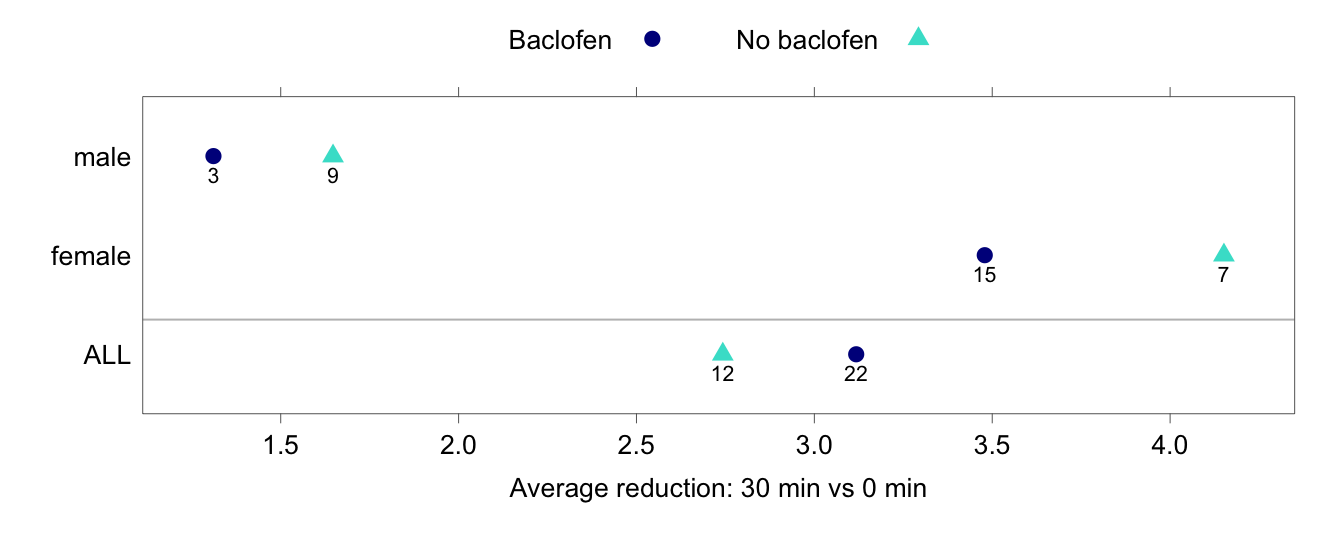
\includegraphics{07-weighting_files/figure-latex/painkiller-1.pdf}
\caption{\label{fig:painkiller}Data are pain reduction scores. Subgroup numbers, shown
below each point, weight the overall average (`'ALL'') for
baclofen towards the high female average, and for no baclofen
slightly towards the low male average.}
\end{figure}

Researchers were comparing two
analgesic treatments, without and with baclofen. When the paper was
first submitted for publication, an alert reviewer spotted that some
of the treatment groups contained more women than men, and asked
whether this might account for the
results.\footnote{Cohen, P. 1996. Pain discriminates between the
sexes.  New Scientist, 2 November, p. 16.}

For a fair overall comparison:

\begin{itemize}
\tightlist
\item
  Calculate means for each subgroup separately.
\item
  Overall treatment effect is average of subgroup differences.
\end{itemize}

The effect of baclofen (reduction in pain score from time 0) is then:

\begin{itemize}
\tightlist
\item
  Females: 3.479 - 4.151 = -0.672 (-ve, therefore an increase)
\item
  Males: 1.311 - 1.647 = -0.336
\item
  Average, male \& female = -0.5 \(\times\) (0.672+0.336) = -0.504
\end{itemize}

\hypertarget{web-page-revenue-per-click-smith-p.111}{%
\subsection*{Web page revenue per click (Smith, p.111)}\label{web-page-revenue-per-click-smith-p.111}}
\addcontentsline{toc}{subsection}{Web page revenue per click (Smith, p.111)}

In 2010 a US Internet company collected data on the effectiveness
of two different web page layouts:

\begin{itemize}
\tightlist
\item
  1-click: Adverts appear on website's first page
\item
  2-click: Click on keyword sends user to page with advert

  \begin{itemize}
  \tightlist
  \item
    Check interest, then show advert
  \end{itemize}
\end{itemize}

\begin{longtable}[]{@{}llllllll@{}}
\toprule
1-click & & & & 2-click & & & \\
\midrule
\endhead
Revenue & Users & RPM & & Revenue & Users & RPM & \\
\$2.9 & 250 & \$11.60 & & \$1.7 & 140 & \$12.14 & \\
\bottomrule
\end{longtable}

\begin{itemize}
\tightlist
\item
  Revenue and users are millions
\item
  RPM is revenue per million users
\end{itemize}

The data combines US and International users. Is that an issue?

\hypertarget{us-vs-international-users}{%
\subsection*{US vs International users}\label{us-vs-international-users}}
\addcontentsline{toc}{subsection}{US vs International users}

\begin{tabular}{l r r r r r r r}
& \multicolumn{3}{l}{1-click} & & \multicolumn{3}{l}{2-click}\\
Location   & Revenue & Users   & RPM && Revenue & Users & RPM\\
US & \$1.8   & \textcolor{red}{70}  &\$27.71 && \$1.2 & \textcolor{red}{50}  & \$24.00\\
Int. & \$1.1   & \textcolor{red}{180} &\$6.11  && \$0.50 & \textcolor{red}{90} & \$5.56\\
& \multicolumn{3}{c}{$\frac{180}{70}$=\textcolor{red}{2.57}} & & \multicolumn{3}{c}{$\frac{90}{50}$=\textcolor{red}{1.8}}\\
\end{tabular}

\begin{itemize}
\tightlist
\item
  Revenue and users are millions
\item
  RPM is revenue per million users
\end{itemize}

This was followed up with a randomized experiment (an A/B test.)

\hypertarget{cricket-bowling-averages}{%
\section{Cricket Bowling Averages}\label{cricket-bowling-averages}}

\hypertarget{runs-r-wickets-w-and-runs-per-wicket}{%
\subsection*{\texorpdfstring{Runs (R), wickets (W) and runs per wicket (\{\em RPW\})}{Runs (R), wickets (W) and runs per wicket (\{\})}}\label{runs-r-wickets-w-and-runs-per-wicket}}
\addcontentsline{toc}{subsection}{Runs (R), wickets (W) and runs per wicket (\{\em RPW\})}

\vspace*{-8pt}

\begin{center}
\begin{tabular}{lrrr||rrr||rrr}
\hline
 & \multicolumn{3}{c}{1st innings} & \multicolumn{3}{c}{2nd innings} &
\multicolumn{3}{c}{Overall} \\
\cline{2-4} \cline{5-7} \cline{8-10}
& R & W & {\em RPW}   & R & W & {\em RPW} & R & W
& {\em RPW}\\
Bowler A & 40 & 4 & {\em 10.0} & 240 & 6 & {\em 40.0} & 280 & 10 &
{\em 28.0}\\
Bowler B & 70 & 5 & {\em 14.0} & 50 & 1 & {\em 50.0} & 120 & 6 & {\em 20.0} \\
\hline
\end{tabular}
\end{center}

\hypertarget{fair-comparison-compare-runs-per-wicket}{%
\subsection*{\texorpdfstring{Fair comparison: Compare runs per wicket (\{\em RPW\})}{Fair comparison: Compare runs per wicket (\{\})}}\label{fair-comparison-compare-runs-per-wicket}}
\addcontentsline{toc}{subsection}{Fair comparison: Compare runs per wicket (\{\em RPW\})}

\vspace*{-5pt}

\begin{center}
\begin{tabular}{lrr||rr||rr}
\hline
 & \multicolumn{2}{c}{1st innings} & \multicolumn{2}{c}{2nd innings} &
\multicolumn{2}{c}{Overall} \\
\cline{2-3} \cline{4-5} \cline{6-7}
         &  RPW & {\em W}   &  RPW & {\em W} &
           RPW & {\em W} \\[4pt]
Bowler A &  10.0 & (4) & 40.0 & (6)  &
$\frac{10+40}{2} = 25$ & (10)\\[4pt]
Bowler B & 14.0 & (5)  & 50.0 & (1) & $\frac{50+14}{2} = 32$  &  (6)\\[4pt]
\cline{2-3} \cline{4-5} \cline{6-7}
\end{tabular}
\end{center}

\hypertarget{epistatic-effects-on-genetic-studies}{%
\section{Epistatic effects on genetic studies}\label{epistatic-effects-on-genetic-studies}}

In population genetics, Simpson's paradox type effects are known as
epistasis. Most human societies are genetically heterogeneous. In
San Francisco, any gene that is different between the European and
Chinese populations will be found to be associated with the use of
chopsticks! If a disease differs in frequency between the European
and Chinese populations, then a naive analysis will find an
association between that disease and any gene that differs in
frequency between the European and Chinese populations.

Such effects are major issues for gene/disease population
association studies. It is now common to collect genetic
fingerprinting data that should identify major heterogeneity.
Providing such differences are accounted for, large effects that show
up in large studies are likely to be real. Small effects may well be
epistatic.

\hypertarget{sec:reg}{%
\chapter{Regression and Correlation}\label{sec:reg}}

Yule-Simpson type effects, discussed in Section \ref{sec:yule1}
{[}``Explaining the Yule-Simpson Paradox''{]}, are important in a
regression context also. Nonsense correlations that arise
where the third variable is time provide simple examples.

\hypertarget{what-direction-does-the-correlation-go}{%
\section{What direction does the correlation go?}\label{what-direction-does-the-correlation-go}}

Variable A may cause variable B. Or variable B may cause
variable A. Or both A and B may be caused (or driven) by
a third variable C. Cases where the third variable is time,
as in Figure \ref{fig:socAnti}, are a fruitful source
of examples of spurious correlations.\footnote{Figure \ref{fig:socAnti}
  is one of many such examples that are available from\\
  \url{http://www.tylervigen.com/spurious-correlations}.}

\begin{Shaded}
\begin{Highlighting}[]
\NormalTok{cap11 }\OtherTok{\textless{}{-}} \StringTok{"Sociology PhDs awarded (from US National Science }
\StringTok{Foundation data) vs Deaths from Anticoagulants.}
\StringTok{"}
\end{Highlighting}
\end{Shaded}

\begin{Shaded}
\begin{Highlighting}[]
\FunctionTok{suppressPackageStartupMessages}\NormalTok{(}\FunctionTok{library}\NormalTok{(latticeExtra))}
\NormalTok{phdDeaths }\OtherTok{\textless{}{-}} \FunctionTok{data.frame}\NormalTok{(}\AttributeTok{Year =} \DecValTok{1999}\SpecialCharTok{:}\DecValTok{2009}\NormalTok{,}
\AttributeTok{Doctorates =} \FunctionTok{c}\NormalTok{(}\DecValTok{572}\NormalTok{,}\DecValTok{617}\NormalTok{,}\DecValTok{566}\NormalTok{,}\DecValTok{547}\NormalTok{,}\DecValTok{597}\NormalTok{,}\DecValTok{580}\NormalTok{,}\DecValTok{536}\NormalTok{,}\DecValTok{579}\NormalTok{,}\DecValTok{576}\NormalTok{,}\DecValTok{601}\NormalTok{,}\DecValTok{664}\NormalTok{),}
\AttributeTok{Deaths =} \FunctionTok{c}\NormalTok{(}\DecValTok{17}\NormalTok{,}\DecValTok{39}\NormalTok{,}\DecValTok{39}\NormalTok{,}\DecValTok{27}\NormalTok{,}\DecValTok{44}\NormalTok{,}\DecValTok{46}\NormalTok{,}\DecValTok{29}\NormalTok{,}\DecValTok{42}\NormalTok{,}\DecValTok{47}\NormalTok{,}\DecValTok{52}\NormalTok{,}\DecValTok{78}\NormalTok{))}
\NormalTok{obj1 }\OtherTok{\textless{}{-}} \FunctionTok{xyplot}\NormalTok{(Doctorates }\SpecialCharTok{\textasciitilde{}}\NormalTok{ Year, }\AttributeTok{data=}\NormalTok{phdDeaths, }\AttributeTok{type=}\StringTok{"b"}\NormalTok{, }\AttributeTok{xlab=}\StringTok{""}\NormalTok{)}
\NormalTok{obj2 }\OtherTok{\textless{}{-}} \FunctionTok{xyplot}\NormalTok{(Deaths }\SpecialCharTok{\textasciitilde{}}\NormalTok{ Year, }\AttributeTok{data=}\NormalTok{phdDeaths, }\AttributeTok{type=}\StringTok{"b"}\NormalTok{)}
\FunctionTok{update}\NormalTok{(}\FunctionTok{doubleYScale}\NormalTok{(obj1, obj2, }\AttributeTok{add.ylab2=}\ConstantTok{TRUE}\NormalTok{),}
       \AttributeTok{par.settings=}\FunctionTok{simpleTheme}\NormalTok{(}\AttributeTok{col=}\FunctionTok{c}\NormalTok{(}\StringTok{"purple"}\NormalTok{,}\StringTok{"black"}\NormalTok{),}
                                \AttributeTok{pch=}\DecValTok{16}\NormalTok{, }\AttributeTok{cex=}\DecValTok{2}\NormalTok{))}
\end{Highlighting}
\end{Shaded}

\begin{figure}
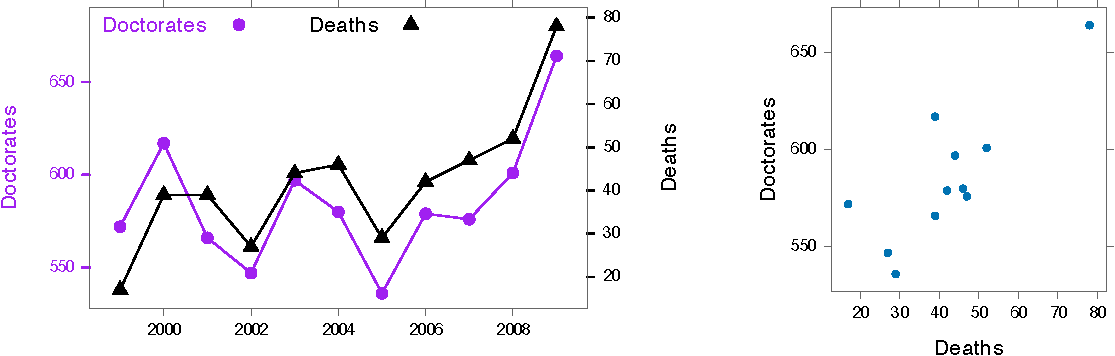
\includegraphics[width=0.75\linewidth]{08-regress_files/figure-latex/socAnti-1} \caption{Sociology PhDs awarded (from US National Science 
Foundation data) vs Deaths from Anticoagulants.
}\label{fig:socAnti}
\end{figure}

Examples of this type help highlight how correlation can and
cannot reasonably be used.

The following examples, where third variables are likely to
be involved, are from \citep[pages 133-134]{nisbett}.

\begin{enumerate}
\def\labelenumi{\arabic{enumi}.}
\tightlist
\item
  Children of parents who try to control eating are more likely
  to be overweight.
\item
  Countries with higher IQs have higher average wealth measures.
\item
  People who smoke marijuana are more likely to later use cocaine.
\item
  Ice cream consumption \& polio were closely correlated in the 1950s.
\end{enumerate}

\hypertarget{regression-to-the-mean}{%
\section{Regression to the mean}\label{regression-to-the-mean}}

Tall fathers are likely to have tall sons, but shorter than themselves.
Tall sons are likely to have tall fathers, but shorter than themselves.
The data shown in Figure \ref{fig:pearson} are from Karl Pearson.
See \texttt{?HistData::PearsonLee}.

\begin{Shaded}
\begin{Highlighting}[]
\NormalTok{cap12 }\OtherTok{\textless{}{-}} \StringTok{"Tall fathers are likely to have tall sons, but shorter than themselves. }
\StringTok{Tall sons are likely to have tall fathers, but shorter than themselves."}
\end{Highlighting}
\end{Shaded}

\begin{Shaded}
\begin{Highlighting}[]
\FunctionTok{par}\NormalTok{(}\AttributeTok{mar=}\FunctionTok{c}\NormalTok{(}\FloatTok{3.6}\NormalTok{,}\FloatTok{3.6}\NormalTok{,}\FloatTok{2.1}\NormalTok{, }\FloatTok{1.1}\NormalTok{), }\AttributeTok{mgp=}\FunctionTok{c}\NormalTok{(}\DecValTok{2}\NormalTok{,}\FloatTok{0.5}\NormalTok{,}\DecValTok{0}\NormalTok{))}
\NormalTok{ptCol }\OtherTok{\textless{}{-}} \FunctionTok{adjustcolor}\NormalTok{(}\StringTok{\textquotesingle{}black\textquotesingle{}}\NormalTok{, }\AttributeTok{alpha=}\FloatTok{0.4}\NormalTok{)}
\FunctionTok{load}\NormalTok{(}\StringTok{\textquotesingle{}Data/Pearson.RData\textquotesingle{}}\NormalTok{)}
\NormalTok{ptCol }\OtherTok{\textless{}{-}} \FunctionTok{adjustcolor}\NormalTok{(}\StringTok{\textquotesingle{}black\textquotesingle{}}\NormalTok{, }\AttributeTok{alpha=}\FloatTok{0.4}\NormalTok{)}
\FunctionTok{plot}\NormalTok{(Pearson[,}\DecValTok{1}\SpecialCharTok{:}\DecValTok{2}\NormalTok{], }\AttributeTok{col=}\NormalTok{ptCol, }\AttributeTok{xlab=}\StringTok{"Father\textquotesingle{}s height (in)"}\NormalTok{, }\AttributeTok{ylab=}\StringTok{"Son\textquotesingle{}s height (in)"}\NormalTok{)}
\NormalTok{avSon }\OtherTok{\textless{}{-}} \FunctionTok{mean}\NormalTok{(Pearson}\SpecialCharTok{$}\NormalTok{Son)}
\NormalTok{avFather }\OtherTok{\textless{}{-}} \FunctionTok{mean}\NormalTok{(Pearson}\SpecialCharTok{$}\NormalTok{Father)}
\FunctionTok{points}\NormalTok{(avFather, avSon, }\AttributeTok{cex=}\FloatTok{1.5}\NormalTok{, }\AttributeTok{col=}\DecValTok{2}\NormalTok{, }\AttributeTok{pch=}\DecValTok{16}\NormalTok{)}
\NormalTok{r }\OtherTok{\textless{}{-}} \FunctionTok{cor}\NormalTok{(Pearson)[}\DecValTok{1}\NormalTok{,}\DecValTok{2}\NormalTok{]}
\FunctionTok{text}\NormalTok{(}\FloatTok{60.5}\NormalTok{,}\DecValTok{77}\NormalTok{, }\FunctionTok{paste}\NormalTok{(}\StringTok{"r ="}\NormalTok{, }\FunctionTok{round}\NormalTok{(r,}\DecValTok{2}\NormalTok{)))}
\NormalTok{Pearson.lm }\OtherTok{\textless{}{-}} \FunctionTok{lm}\NormalTok{(Son}\SpecialCharTok{\textasciitilde{}}\NormalTok{Father, }\AttributeTok{data=}\NormalTok{Pearson)}
\NormalTok{b }\OtherTok{\textless{}{-}} \FunctionTok{coef}\NormalTok{(Pearson.lm)}
\NormalTok{pc95 }\OtherTok{\textless{}{-}} \FunctionTok{quantile}\NormalTok{(Pearson}\SpecialCharTok{$}\NormalTok{Father, }\FloatTok{0.95}\NormalTok{)}
\NormalTok{son95 }\OtherTok{\textless{}{-}} \FunctionTok{quantile}\NormalTok{(Pearson}\SpecialCharTok{$}\NormalTok{Son, }\FloatTok{0.95}\NormalTok{)}
\NormalTok{pred95 }\OtherTok{\textless{}{-}}\NormalTok{ b[}\DecValTok{1}\NormalTok{]}\SpecialCharTok{+}\NormalTok{b[}\DecValTok{2}\NormalTok{]}\SpecialCharTok{*}\NormalTok{pc95}
\FunctionTok{abline}\NormalTok{(Pearson.lm, }\AttributeTok{col=}\DecValTok{2}\NormalTok{)}
\FunctionTok{abline}\NormalTok{(}\AttributeTok{v=}\NormalTok{pc95, }\AttributeTok{col=}\DecValTok{2}\NormalTok{)}
\FunctionTok{abline}\NormalTok{(}\AttributeTok{h=}\NormalTok{pred95, }\AttributeTok{col=}\DecValTok{2}\NormalTok{)}
\FunctionTok{abline}\NormalTok{(}\AttributeTok{h=}\NormalTok{son95, }\AttributeTok{col=}\DecValTok{2}\NormalTok{, }\AttributeTok{lty=}\DecValTok{2}\NormalTok{)}
\NormalTok{pcSon }\OtherTok{\textless{}{-}} \FunctionTok{round}\NormalTok{(}\DecValTok{100}\SpecialCharTok{*}\FunctionTok{with}\NormalTok{(Pearson, }\FunctionTok{sum}\NormalTok{(Son}\SpecialCharTok{\textless{}}\NormalTok{pred95)}\SpecialCharTok{/}\FunctionTok{nrow}\NormalTok{(Pearson)))}
\FunctionTok{mtext}\NormalTok{(}\AttributeTok{side=}\DecValTok{3}\NormalTok{, }\AttributeTok{line=}\FloatTok{0.05}\NormalTok{, }\StringTok{"95th percentile"}\NormalTok{, }\AttributeTok{col=}\DecValTok{2}\NormalTok{, }\AttributeTok{at=}\NormalTok{pc95)}
\FunctionTok{mtext}\NormalTok{(}\AttributeTok{side=}\DecValTok{4}\NormalTok{, }\AttributeTok{line=}\FloatTok{0.85}\NormalTok{, }\FunctionTok{paste0}\NormalTok{(pcSon,}\StringTok{"th}\SpecialCharTok{\textbackslash{}n}\StringTok{percentile"}\NormalTok{), }\AttributeTok{col=}\DecValTok{2}\NormalTok{, }\AttributeTok{at=}\NormalTok{pred95, }\AttributeTok{srt=}\DecValTok{90}\NormalTok{)}
\FunctionTok{mtext}\NormalTok{(}\AttributeTok{side=}\DecValTok{3}\NormalTok{, }\AttributeTok{line=}\FloatTok{1.0}\NormalTok{, }\StringTok{"Son\textquotesingle{}s height, given father\textquotesingle{}s height (red lines)"}\NormalTok{)}
\FunctionTok{plot}\NormalTok{(Pearson[,}\DecValTok{1}\SpecialCharTok{:}\DecValTok{2}\NormalTok{], }\AttributeTok{col=}\NormalTok{ptCol)}
\FunctionTok{text}\NormalTok{(}\FloatTok{60.5}\NormalTok{,}\DecValTok{77}\NormalTok{, }\FunctionTok{paste}\NormalTok{(}\StringTok{"r ="}\NormalTok{, }\FunctionTok{round}\NormalTok{(r,}\DecValTok{2}\NormalTok{)))}
\NormalTok{Pearson.lm2 }\OtherTok{\textless{}{-}} \FunctionTok{lm}\NormalTok{(Father}\SpecialCharTok{\textasciitilde{}}\NormalTok{Son, }\AttributeTok{data=}\NormalTok{Pearson)}
\NormalTok{c2 }\OtherTok{\textless{}{-}} \FunctionTok{coef}\NormalTok{(Pearson.lm2)}
\NormalTok{b2 }\OtherTok{\textless{}{-}} \FunctionTok{c}\NormalTok{(}\SpecialCharTok{{-}}\NormalTok{c2[}\DecValTok{1}\NormalTok{]}\SpecialCharTok{/}\NormalTok{c2[}\DecValTok{2}\NormalTok{], }\DecValTok{1}\SpecialCharTok{/}\NormalTok{c2[}\DecValTok{2}\NormalTok{])}
\NormalTok{son95 }\OtherTok{\textless{}{-}} \FunctionTok{quantile}\NormalTok{(Pearson}\SpecialCharTok{$}\NormalTok{Son, }\FloatTok{0.95}\NormalTok{)}
\NormalTok{predF95 }\OtherTok{\textless{}{-}}\NormalTok{ c2[}\DecValTok{1}\NormalTok{]}\SpecialCharTok{+}\NormalTok{c2[}\DecValTok{2}\NormalTok{]}\SpecialCharTok{*}\NormalTok{son95}
\FunctionTok{abline}\NormalTok{(Pearson.lm, }\AttributeTok{col=}\FunctionTok{adjustcolor}\NormalTok{(}\StringTok{"red"}\NormalTok{,}\AttributeTok{alpha=}\FloatTok{0.4}\NormalTok{))}
\FunctionTok{abline}\NormalTok{(b2, }\AttributeTok{col=}\StringTok{"purple"}\NormalTok{, }\AttributeTok{lty=}\DecValTok{2}\NormalTok{, }\AttributeTok{lwd=}\DecValTok{2}\NormalTok{)}
\FunctionTok{abline}\NormalTok{(}\AttributeTok{h=}\NormalTok{son95, }\AttributeTok{col=}\StringTok{"purple"}\NormalTok{, }\AttributeTok{lty=}\DecValTok{2}\NormalTok{, }\AttributeTok{lwd=}\DecValTok{2}\NormalTok{)}
\FunctionTok{abline}\NormalTok{(}\AttributeTok{v=}\NormalTok{predF95, }\AttributeTok{col=}\StringTok{"purple"}\NormalTok{, }\AttributeTok{lty=}\DecValTok{2}\NormalTok{, }\AttributeTok{lwd=}\DecValTok{2}\NormalTok{)}
\FunctionTok{abline}\NormalTok{(}\AttributeTok{v=}\NormalTok{pc95, }\AttributeTok{col=}\FunctionTok{adjustcolor}\NormalTok{(}\StringTok{\textquotesingle{}red\textquotesingle{}}\NormalTok{,}\AttributeTok{alpha=}\FloatTok{0.4}\NormalTok{))}
\FunctionTok{abline}\NormalTok{(}\AttributeTok{h=}\NormalTok{pred95, }\AttributeTok{col=}\FunctionTok{adjustcolor}\NormalTok{(}\StringTok{\textquotesingle{}red\textquotesingle{}}\NormalTok{,}\AttributeTok{alpha=}\FloatTok{0.4}\NormalTok{))}
\NormalTok{pcF }\OtherTok{\textless{}{-}} \FunctionTok{round}\NormalTok{(}\DecValTok{100}\SpecialCharTok{*}\FunctionTok{with}\NormalTok{(Pearson, }\FunctionTok{sum}\NormalTok{(Father}\SpecialCharTok{\textless{}=}\NormalTok{predF95)}\SpecialCharTok{/}\FunctionTok{nrow}\NormalTok{(Pearson)))}
\FunctionTok{mtext}\NormalTok{(}\AttributeTok{side=}\DecValTok{3}\NormalTok{, }\AttributeTok{line=}\FloatTok{1.0}\NormalTok{, }\StringTok{"Father\textquotesingle{}s height, given son\textquotesingle{}s height (purple lines)"}\NormalTok{)}
\FunctionTok{mtext}\NormalTok{(}\AttributeTok{side=}\DecValTok{3}\NormalTok{, }\AttributeTok{line=}\SpecialCharTok{{-}}\FloatTok{0.25}\NormalTok{, }\FunctionTok{paste0}\NormalTok{(pcF,}\StringTok{"th percentile"}\NormalTok{), }\AttributeTok{col=}\StringTok{"purple"}\NormalTok{, }\AttributeTok{at=}\NormalTok{predF95)}
\FunctionTok{mtext}\NormalTok{(}\AttributeTok{side=}\DecValTok{4}\NormalTok{, }\AttributeTok{line=}\FloatTok{0.05}\NormalTok{, }\FunctionTok{paste0}\NormalTok{(}\StringTok{"95th percentile"}\NormalTok{), }\AttributeTok{col=}\StringTok{"purple"}\NormalTok{, }\AttributeTok{at=}\NormalTok{son95, }\AttributeTok{srt=}\DecValTok{90}\NormalTok{)}
\end{Highlighting}
\end{Shaded}

\begin{figure}
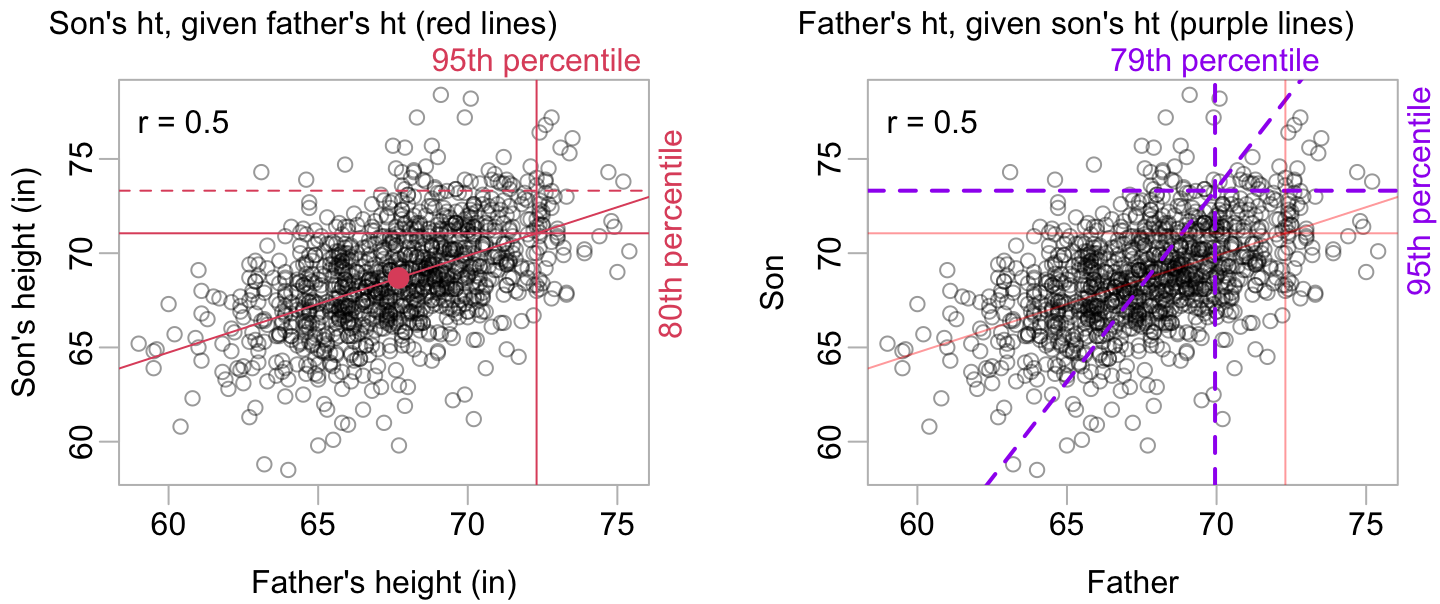
\includegraphics[width=0.48\linewidth]{08-regress_files/figure-latex/pearson-1} 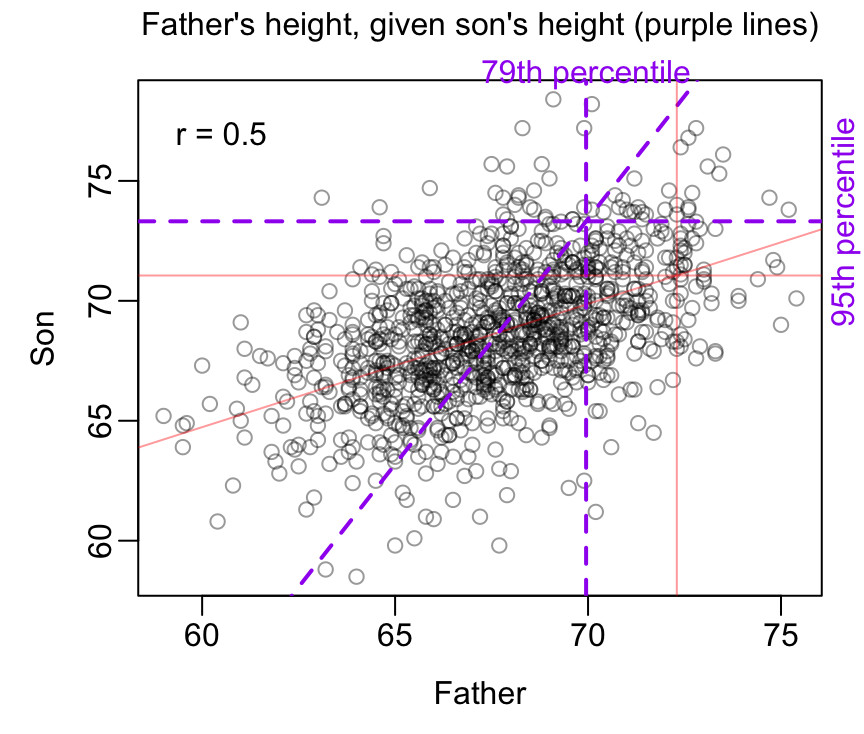
\includegraphics[width=0.48\linewidth]{08-regress_files/figure-latex/pearson-2} \caption{Tall fathers are likely to have tall sons, but shorter than themselves. 
Tall sons are likely to have tall fathers, but shorter than themselves.}\label{fig:pearson}
\end{figure}

Kahneman argues, perhaps too simplistically:

\begin{itemize}
\tightlist
\item
  Height is mainly due to genetic factors
\item
  Sons share half their genes with their fathers
\item
  Hence, correlation between sons' \& fathers' heights \(\simeq\) 0.5
\end{itemize}

\enlargethispage{21pt}

Galton's 1886 data, which predates Pearson's data, shows a 0.46
correlation between child height and the average of the parent
height.

Regression to the mean in verse:\\
\url{https://www.youtube.com/watch?v=sxMllckUWaw}

\hypertarget{kahnemans-comments-on-regression-to-the-mean}{%
\subsection*{Kahneman's comments on regression to the mean}\label{kahnemans-comments-on-regression-to-the-mean}}
\addcontentsline{toc}{subsection}{Kahneman's comments on regression to the mean}

``Extreme predictions and a willingness to predict rare events from
weak evidence are both manifestations of System 1. \ldots{}''\\
``Regression to the mean is also a problem for System 2. The very idea
\ldots{} is alien and difficult to communicate and comprehend. This is a
case where System 2 requires special training.''\\
``We intuitively want to match predictions to the evidence.''\\
``We will not learn to understand regression from experience.''

\hypertarget{regression-to-the-mean-in-a-variety-of-contexts}{%
\section{Regression to the mean in a variety of contexts}\label{regression-to-the-mean-in-a-variety-of-contexts}}

\hypertarget{decathlon-scores-between-event-correlations}{%
\section*{Decathlon scores --- between event correlations}\label{decathlon-scores-between-event-correlations}}
\addcontentsline{toc}{section}{Decathlon scores --- between event correlations}

\begin{Shaded}
\begin{Highlighting}[]
\NormalTok{cap13 }\OtherTok{\textless{}{-}} \StringTok{"Between event correlations for top performances in the decathlon}
\StringTok{between 1985 and 2006."}
\end{Highlighting}
\end{Shaded}

\begin{Shaded}
\begin{Highlighting}[]
\NormalTok{Decath2006 }\OtherTok{\textless{}{-}} \FunctionTok{subset}\NormalTok{(GDAdata}\SpecialCharTok{::}\NormalTok{Decathlon,yearEvent}\SpecialCharTok{==}\DecValTok{2006}\NormalTok{)}
\NormalTok{pointsNam }\OtherTok{\textless{}{-}} \FunctionTok{c}\NormalTok{(}\StringTok{"100m"}\NormalTok{, }\StringTok{"Longjmp"}\NormalTok{, }\StringTok{"Shotput"}\NormalTok{, }\StringTok{"Highjmp"}\NormalTok{, }\StringTok{"400m"}\NormalTok{, }\StringTok{"110mHurd"}\NormalTok{, }
\StringTok{"Discus"}\NormalTok{, }\StringTok{"PVault"}\NormalTok{, }\StringTok{"Javelin"}\NormalTok{, }\StringTok{"1500m"}\NormalTok{)}
\DocumentationTok{\#\# ord \textless{}{-} dput(corrplot::corrMatOrder(cor(Decath2006[,15:24])))}
\NormalTok{ord }\OtherTok{\textless{}{-}} \FunctionTok{c}\NormalTok{(10L, 9L, 8L, 3L, 7L, 4L, 6L, 2L, 1L, 5L)}
\DocumentationTok{\#\# Check difference of rank from Pearson correlations }
\NormalTok{corP }\OtherTok{\textless{}{-}} \FunctionTok{cor}\NormalTok{(Decath2006[,ord}\SpecialCharTok{+}\DecValTok{14}\NormalTok{])}
\NormalTok{corS }\OtherTok{\textless{}{-}} \FunctionTok{cor}\NormalTok{(Decath2006[,ord}\SpecialCharTok{+}\DecValTok{14}\NormalTok{],}\AttributeTok{method=}\StringTok{"spearman"}\NormalTok{)}
\DocumentationTok{\#\# round(corP{-}corS,2)}
\DocumentationTok{\#\# dput(corrplot::corrMatOrder(cor(Decath2006[,15:24])))}
\NormalTok{ord }\OtherTok{\textless{}{-}} \FunctionTok{c}\NormalTok{(10L, 9L, 8L, 3L, 7L, 4L, 6L, 2L, 1L, 5L)}
\end{Highlighting}
\end{Shaded}

\begin{verbatim}
## 
## Attaching package: 'ggplot2'
\end{verbatim}

\begin{verbatim}
## The following object is masked from 'package:latticeExtra':
## 
##     layer
\end{verbatim}

\begin{verbatim}
## Registered S3 method overwritten by 'GGally':
##   method from   
##   +.gg   ggplot2
\end{verbatim}

\begin{Shaded}
\begin{Highlighting}[]
\NormalTok{my\_fn }\OtherTok{\textless{}{-}} \ControlFlowTok{function}\NormalTok{(data, mapping, }\AttributeTok{pts=}\FunctionTok{list}\NormalTok{(), }\AttributeTok{smt=}\FunctionTok{list}\NormalTok{(), ...)\{}
              \FunctionTok{ggplot}\NormalTok{(}\AttributeTok{data =}\NormalTok{ data, }\AttributeTok{mapping =}\NormalTok{ mapping, ...) }\SpecialCharTok{+} 
                         \FunctionTok{do.call}\NormalTok{(geom\_point, pts) }\SpecialCharTok{+}
                         \FunctionTok{do.call}\NormalTok{(geom\_smooth, smt) }
\NormalTok{\}}
\NormalTok{my\_custom\_cor }\OtherTok{\textless{}{-}} \ControlFlowTok{function}\NormalTok{(data, mapping, }\AttributeTok{color =} \FunctionTok{I}\NormalTok{(}\StringTok{"grey50"}\NormalTok{), }\AttributeTok{sizeRange =} \FunctionTok{c}\NormalTok{(}\DecValTok{1}\NormalTok{, }\DecValTok{5}\NormalTok{), ...) \{}

  \CommentTok{\# get the x and y data to use the other code}
\NormalTok{  x }\OtherTok{\textless{}{-}} \FunctionTok{eval\_data\_col}\NormalTok{(data, mapping}\SpecialCharTok{$}\NormalTok{x)}
\NormalTok{  y }\OtherTok{\textless{}{-}} \FunctionTok{eval\_data\_col}\NormalTok{(data, mapping}\SpecialCharTok{$}\NormalTok{y)}
\NormalTok{  ct }\OtherTok{\textless{}{-}} \FunctionTok{cor.test}\NormalTok{(x,y)}

\NormalTok{  r }\OtherTok{\textless{}{-}} \FunctionTok{unname}\NormalTok{(ct}\SpecialCharTok{$}\NormalTok{estimate)}
\NormalTok{  rt }\OtherTok{\textless{}{-}} \FunctionTok{format}\NormalTok{(r, }\AttributeTok{digits=}\DecValTok{2}\NormalTok{)[}\DecValTok{1}\NormalTok{]}

  \CommentTok{\# since we can\textquotesingle{}t print it to get the strsize, just use the max size range}
\NormalTok{  cex }\OtherTok{\textless{}{-}} \FunctionTok{max}\NormalTok{(sizeRange)}

  \CommentTok{\# helper function to calculate a useable size}
\NormalTok{  percent\_of\_range }\OtherTok{\textless{}{-}} \ControlFlowTok{function}\NormalTok{(percent, range) \{}
\NormalTok{    percent }\SpecialCharTok{*} \FunctionTok{diff}\NormalTok{(range) }\SpecialCharTok{+} \FunctionTok{min}\NormalTok{(range, }\AttributeTok{na.rm =} \ConstantTok{TRUE}\NormalTok{)}
\NormalTok{  \}}

  \CommentTok{\# plot the cor value}
  \FunctionTok{ggally\_text}\NormalTok{(}
    \AttributeTok{label =} \FunctionTok{as.character}\NormalTok{(rt), }
    \AttributeTok{mapping =} \FunctionTok{aes}\NormalTok{(),}
    \AttributeTok{xP =} \FloatTok{0.5}\NormalTok{, }\AttributeTok{yP =} \FloatTok{0.5}\NormalTok{, }
    \AttributeTok{size =} \FunctionTok{I}\NormalTok{(}\FunctionTok{percent\_of\_range}\NormalTok{(cex }\SpecialCharTok{*} \FunctionTok{abs}\NormalTok{(r), sizeRange)),}
    \AttributeTok{color =}\NormalTok{ color,}
\NormalTok{    ...}
\NormalTok{  )  }\SpecialCharTok{+} 
    \CommentTok{\# remove all the background stuff and wrap it with a dashed line}
    \FunctionTok{theme\_classic}\NormalTok{() }\SpecialCharTok{+} 
    \FunctionTok{theme}\NormalTok{(}
      \AttributeTok{panel.background =} \FunctionTok{element\_rect}\NormalTok{(}
        \AttributeTok{color =}\NormalTok{ color, }
        \AttributeTok{linetype =} \StringTok{"longdash"}
\NormalTok{      ), }
      \AttributeTok{axis.line =} \FunctionTok{element\_blank}\NormalTok{(), }
      \AttributeTok{axis.ticks =} \FunctionTok{element\_blank}\NormalTok{(), }
      \AttributeTok{axis.text.y =} \FunctionTok{element\_blank}\NormalTok{(), }
      \AttributeTok{axis.text.x =} \FunctionTok{element\_blank}\NormalTok{()}
\NormalTok{    )}
\NormalTok{\}}

\FunctionTok{ggpairs}\NormalTok{(Decath2006[,(}\DecValTok{15}\SpecialCharTok{:}\DecValTok{24}\NormalTok{)[ord]], }
        \AttributeTok{lower =} \FunctionTok{list}\NormalTok{(}\AttributeTok{continuous =} 
                       \FunctionTok{wrap}\NormalTok{(my\_fn,}
                            \AttributeTok{pts=}\FunctionTok{list}\NormalTok{(}\AttributeTok{size=}\FloatTok{0.25}\NormalTok{, }\AttributeTok{colour=}\FunctionTok{adjustcolor}\NormalTok{(}\StringTok{"black"}\NormalTok{, }\AttributeTok{alpha=}\FloatTok{0.4}\NormalTok{)), }
                            \AttributeTok{smt=}\FunctionTok{list}\NormalTok{(}\AttributeTok{method=}\StringTok{"gam"}\NormalTok{, }\AttributeTok{se=}\NormalTok{F, }\AttributeTok{size=}\FloatTok{0.5}\NormalTok{, }\AttributeTok{colour=}\StringTok{"red"}\NormalTok{))),}
        \AttributeTok{axisLabels=}\StringTok{"none"}\NormalTok{, }\AttributeTok{columnLabels=}\NormalTok{pointsNam,}
        \AttributeTok{upper=}\FunctionTok{list}\NormalTok{(}\AttributeTok{continuous=}\FunctionTok{wrap}\NormalTok{(my\_custom\_cor, }\AttributeTok{sizeRange=}\FunctionTok{c}\NormalTok{(}\FloatTok{2.5}\NormalTok{,}\FloatTok{4.5}\NormalTok{))))}
\end{Highlighting}
\end{Shaded}

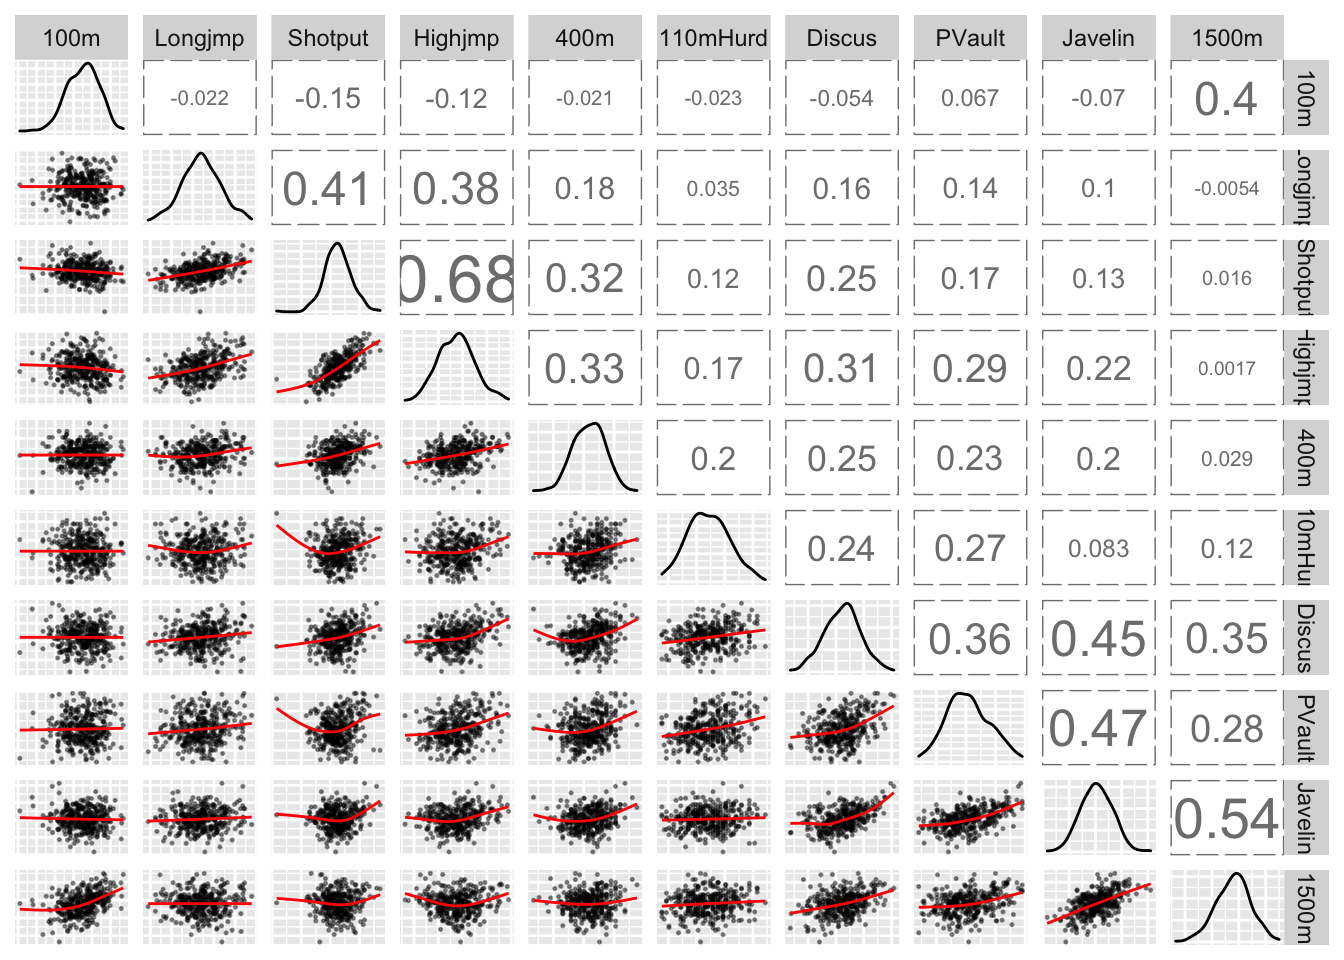
\includegraphics{08-regress_files/figure-latex/gg-1.pdf}

The dataset \texttt{GDAdata::Decathlon} has best annual performances of 6800 points and over for a twenty-one year period after new rules were introduced in
1985.\footnote{Data are from the Estonian website \url{http://www.decathlon2000.com/}}

\hypertarget{plot-measures-not-points-selection-only}{%
\subsection*{Plot measures, not points (selection only)}\label{plot-measures-not-points-selection-only}}
\addcontentsline{toc}{subsection}{Plot measures, not points (selection only)}

\begin{Shaded}
\begin{Highlighting}[]
\NormalTok{choosecols }\OtherTok{\textless{}{-}}\NormalTok{ ord[}\DecValTok{5}\SpecialCharTok{:}\DecValTok{9}\NormalTok{]}
\FunctionTok{ggpairs}\NormalTok{(Decath2006[, (}\DecValTok{4}\SpecialCharTok{:}\DecValTok{13}\NormalTok{)[choosecols]],}
        \AttributeTok{lower =} \FunctionTok{list}\NormalTok{(}\AttributeTok{continuous =} 
                       \FunctionTok{wrap}\NormalTok{(my\_fn,}
                            \AttributeTok{pts=}\FunctionTok{list}\NormalTok{(}\AttributeTok{size=}\FloatTok{0.25}\NormalTok{, }\AttributeTok{colour=}\FunctionTok{adjustcolor}\NormalTok{(}\StringTok{"black"}\NormalTok{, }\AttributeTok{alpha=}\FloatTok{0.4}\NormalTok{)), }
                            \AttributeTok{smt=}\FunctionTok{list}\NormalTok{(}\AttributeTok{method=}\StringTok{"gam"}\NormalTok{, }\AttributeTok{se=}\NormalTok{F, }\AttributeTok{size=}\FloatTok{0.5}\NormalTok{, }\AttributeTok{colour=}\StringTok{"red"}\NormalTok{))),}
        \AttributeTok{columnLabels=}\NormalTok{pointsNam[}\DecValTok{5}\SpecialCharTok{:}\DecValTok{9}\NormalTok{],}
        \AttributeTok{upper=}\FunctionTok{list}\NormalTok{(}\AttributeTok{continuous=}\FunctionTok{wrap}\NormalTok{(my\_custom\_cor, }\AttributeTok{sizeRange=}\FunctionTok{c}\NormalTok{(}\DecValTok{3}\NormalTok{,}\DecValTok{5}\NormalTok{))))}
\end{Highlighting}
\end{Shaded}

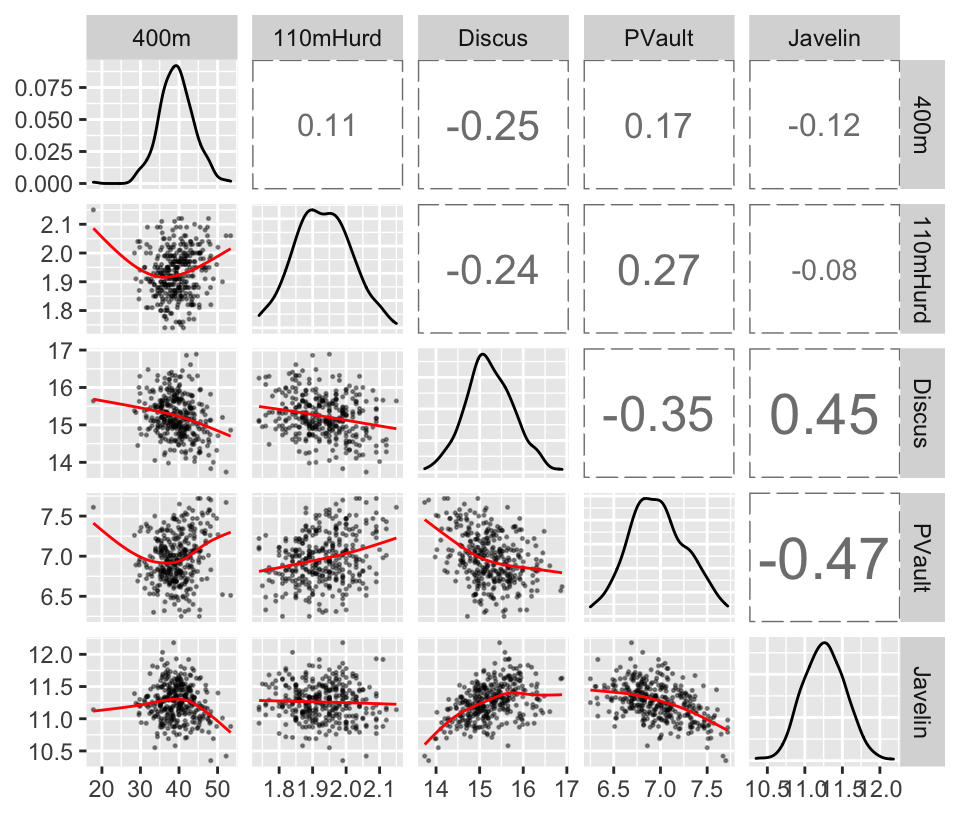
\includegraphics[width=0.8\linewidth]{08-regress_files/figure-latex/select-1}

\hypertarget{total-profit-to-total-income-ratio-by-industry-class}{%
\subsection*{Total profit to total income ratio, by industry class}\label{total-profit-to-total-income-ratio-by-industry-class}}
\addcontentsline{toc}{subsection}{Total profit to total income ratio, by industry class}

Data are from the Statistics NZ Business Performance
Benchmarker\footnote{\url{https://shinyapps.stats.govt.nz/bpb/}}

\begin{Shaded}
\begin{Highlighting}[]
\NormalTok{cap14 }\OtherTok{\textless{}{-}} \FunctionTok{paste}\NormalTok{(}\StringTok{"Total profit to total income ratio, by industry class {-}{-}{-}"}\NormalTok{,}
\StringTok{"correlation between 2015 value and 2013 value."}\NormalTok{)}
\end{Highlighting}
\end{Shaded}

\begin{Shaded}
\begin{Highlighting}[]
\FunctionTok{load}\NormalTok{(}\StringTok{\textquotesingle{}data/FinAllInd.RData\textquotesingle{}}\NormalTok{)}
\NormalTok{expend }\OtherTok{\textless{}{-}} \FunctionTok{subset}\NormalTok{(FinAllInd, }\AttributeTok{subset=}\NormalTok{Variable}\SpecialCharTok{==}\StringTok{"Expenditure"}\NormalTok{)}
\NormalTok{profit }\OtherTok{\textless{}{-}} \FunctionTok{subset}\NormalTok{(FinAllInd, }\AttributeTok{subset=}\NormalTok{Variable}\SpecialCharTok{==}\StringTok{"Profit"}\NormalTok{)}
\NormalTok{income }\OtherTok{\textless{}{-}} \FunctionTok{subset}\NormalTok{(FinAllInd, }\AttributeTok{subset=}\NormalTok{Variable}\SpecialCharTok{==}\StringTok{"Income"}\NormalTok{)}
\NormalTok{assets }\OtherTok{\textless{}{-}} \FunctionTok{subset}\NormalTok{(FinAllInd, }\AttributeTok{subset=}\NormalTok{Variable}\SpecialCharTok{==}\StringTok{"Assets"}\NormalTok{)}
\NormalTok{employ }\OtherTok{\textless{}{-}} \FunctionTok{subset}\NormalTok{(FinAllInd, }\AttributeTok{subset=}\NormalTok{Variable}\SpecialCharTok{==}\StringTok{"Employee Count"}\NormalTok{)}
\CommentTok{\# expend[,6] \textless{}{-} as.numeric(expend[[6]])}
\CommentTok{\# expend[,7] \textless{}{-} as.numeric(expend[[7]])}
\CommentTok{\# expend[,8] \textless{}{-} as.numeric(expend[[8]])}
\FunctionTok{plot}\NormalTok{(}\FunctionTok{I}\NormalTok{(profit[[}\DecValTok{9}\NormalTok{]]}\SpecialCharTok{/}\NormalTok{income[[}\DecValTok{9}\NormalTok{]])}\SpecialCharTok{\textasciitilde{}}\FunctionTok{I}\NormalTok{(profit[[}\DecValTok{11}\NormalTok{]]}\SpecialCharTok{/}\NormalTok{income[[}\DecValTok{11}\NormalTok{]]), }
     \AttributeTok{pch=}\DecValTok{16}\NormalTok{, }\AttributeTok{cex=}\FloatTok{1.25}\NormalTok{, }\AttributeTok{xlab=}\StringTok{"2013 ratio"}\NormalTok{, }\AttributeTok{ylab=}\StringTok{"2015 ratio"}\NormalTok{,}
     \AttributeTok{cex.lab=}\FloatTok{1.55}\NormalTok{, }\AttributeTok{col=}\FunctionTok{adjustcolor}\NormalTok{(}\StringTok{\textquotesingle{}purple\textquotesingle{}}\NormalTok{,}\AttributeTok{alpha=}\FloatTok{0.5}\NormalTok{), }\AttributeTok{fg=}\StringTok{"gray"}\NormalTok{,}
     \AttributeTok{xlim=}\FunctionTok{c}\NormalTok{(}\SpecialCharTok{{-}}\FloatTok{0.15}\NormalTok{,}\FloatTok{0.475}\NormalTok{), }\AttributeTok{ylim=}\FunctionTok{c}\NormalTok{(}\SpecialCharTok{{-}}\FloatTok{0.125}\NormalTok{, }\FloatTok{0.41}\NormalTok{))}
\FunctionTok{mtext}\NormalTok{(}\AttributeTok{side=}\DecValTok{3}\NormalTok{, }\AttributeTok{line=}\FloatTok{0.5}\NormalTok{, }\StringTok{"Total profit to total income ratio"}\NormalTok{)}
\FunctionTok{par}\NormalTok{(}\AttributeTok{xpd=}\ConstantTok{TRUE}\NormalTok{)}
\NormalTok{rt }\OtherTok{\textless{}{-}} \FunctionTok{c}\NormalTok{(}\DecValTok{31}\NormalTok{,}\DecValTok{37}\NormalTok{,}\DecValTok{167}\NormalTok{, }\DecValTok{330}\NormalTok{, }\DecValTok{385}\NormalTok{, }\DecValTok{441}\NormalTok{, }\DecValTok{458}\NormalTok{)}
\NormalTok{left }\OtherTok{\textless{}{-}} \FunctionTok{c}\NormalTok{(}\DecValTok{10}\NormalTok{, }\DecValTok{15}\NormalTok{, }\DecValTok{35}\NormalTok{, }\DecValTok{57}\NormalTok{, }\DecValTok{76}\NormalTok{,}\DecValTok{122}\NormalTok{,}\DecValTok{157}\NormalTok{,}\DecValTok{175}\NormalTok{, }\DecValTok{164}\NormalTok{, }\DecValTok{196}\NormalTok{, }\DecValTok{253}\NormalTok{, }\DecValTok{274}\NormalTok{, }\DecValTok{292}\NormalTok{,}\DecValTok{341}\NormalTok{,}\DecValTok{362}\NormalTok{, }\DecValTok{384}\NormalTok{,}\DecValTok{430}\NormalTok{)}
\NormalTok{halfblack }\OtherTok{\textless{}{-}} \FunctionTok{adjustcolor}\NormalTok{(}\StringTok{\textquotesingle{}black\textquotesingle{}}\NormalTok{, }\AttributeTok{alpha=}\FloatTok{0.35}\NormalTok{)}
\NormalTok{df }\OtherTok{\textless{}{-}} \FunctionTok{data.frame}\NormalTok{(}\AttributeTok{ratio15=}\FunctionTok{I}\NormalTok{(profit[[}\DecValTok{9}\NormalTok{]]}\SpecialCharTok{/}\NormalTok{income[[}\DecValTok{9}\NormalTok{]]), }\AttributeTok{ratio13=}\FunctionTok{I}\NormalTok{(profit[[}\DecValTok{11}\NormalTok{]]}\SpecialCharTok{/}\NormalTok{income[[}\DecValTok{11}\NormalTok{]]),}
                 \AttributeTok{indclass=}\NormalTok{profit[[}\StringTok{"Industry\_class"}\NormalTok{]])}
\FunctionTok{with}\NormalTok{(df[rt,], }\FunctionTok{text}\NormalTok{(ratio15}\SpecialCharTok{\textasciitilde{}}\NormalTok{ratio13,}\AttributeTok{col=}\NormalTok{halfblack,}\AttributeTok{labels=}\NormalTok{indclass,}\AttributeTok{pos=}\DecValTok{2}\NormalTok{))}
\FunctionTok{with}\NormalTok{(df[left,], }\FunctionTok{text}\NormalTok{(ratio15}\SpecialCharTok{\textasciitilde{}}\NormalTok{ratio13,}\AttributeTok{col=}\NormalTok{halfblack,}\AttributeTok{labels=}\NormalTok{indclass,}\AttributeTok{pos=}\DecValTok{4}\NormalTok{))}
\end{Highlighting}
\end{Shaded}

\begin{figure}[H]
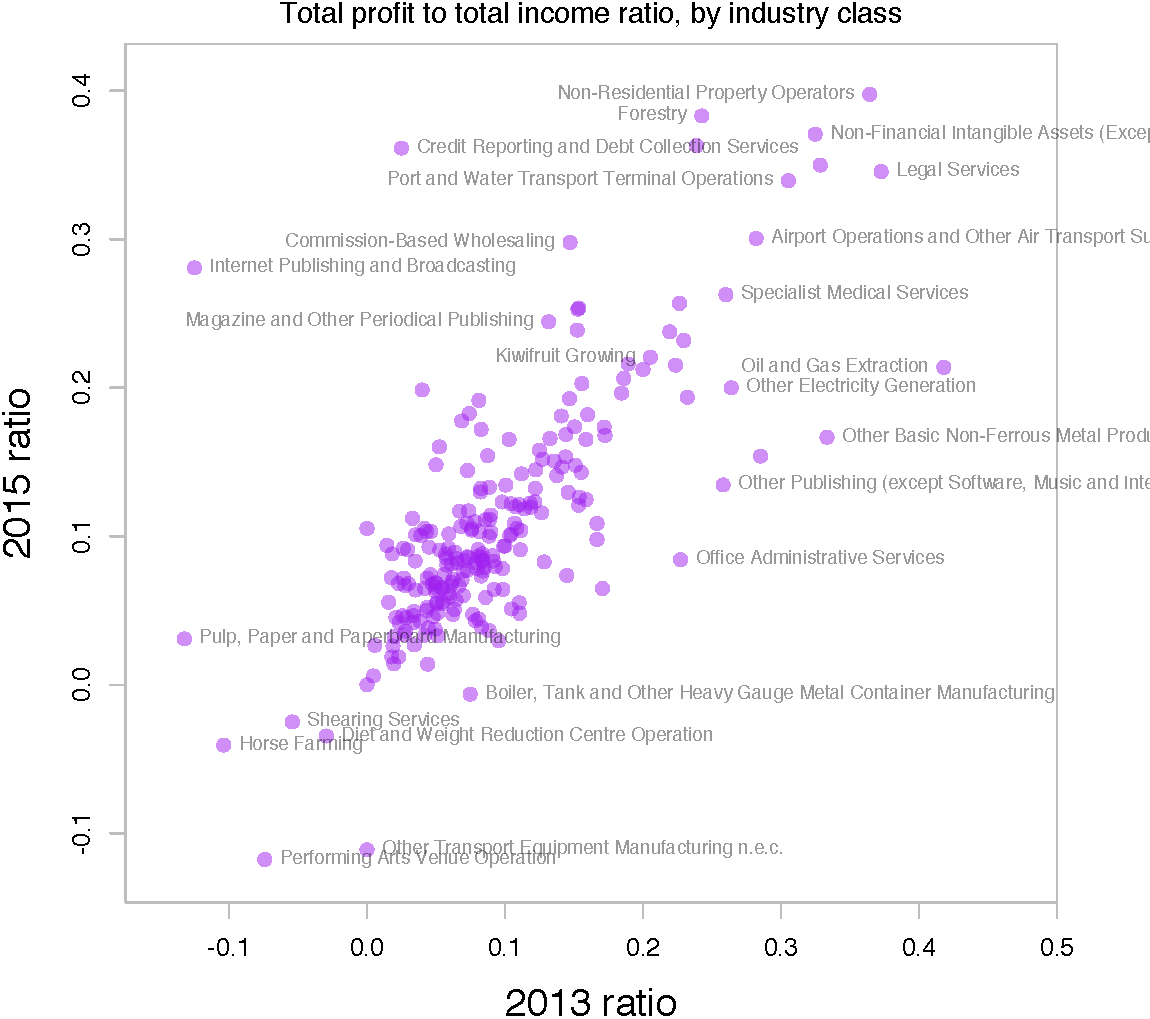
\includegraphics[width=0.8\linewidth]{08-regress_files/figure-latex/expend-1} \caption{Total profit to total income ratio, by industry class --- correlation between 2015 value and 2013 value.}\label{fig:expend}
\end{figure}

Not shown are 4 points where the 2015 ratio was less than -0.3.\\
(Olive growing, Petroleum exploration, Stevedoring Services.)

\hypertarget{nba-player-total-points-correlations-decline-over-time}{%
\subsection*{NBA player total points --- correlations decline over time}\label{nba-player-total-points-correlations-decline-over-time}}
\addcontentsline{toc}{subsection}{NBA player total points --- correlations decline over time}

\begin{Shaded}
\begin{Highlighting}[]
\NormalTok{cap12}\FloatTok{.5} \OtherTok{\textless{}{-}} \StringTok{"As time progresses, correlation decreases, and regression to the mean increases."}
\end{Highlighting}
\end{Shaded}

\begin{Shaded}
\begin{Highlighting}[]
\FunctionTok{load}\NormalTok{(}\StringTok{"data/NBAplayer.RData"}\NormalTok{)}
\NormalTok{m1516 }\OtherTok{\textless{}{-}} \FunctionTok{with}\NormalTok{(NBAplayer, }\FunctionTok{match}\NormalTok{(z15}\SpecialCharTok{$}\NormalTok{Name,z16}\SpecialCharTok{$}\NormalTok{Name,}\AttributeTok{nomatch=}\DecValTok{0}\NormalTok{))}
\NormalTok{df }\OtherTok{\textless{}{-}} \FunctionTok{with}\NormalTok{(NBAplayer, }\FunctionTok{data.frame}\NormalTok{(}\AttributeTok{p1516=}\NormalTok{z15}\SpecialCharTok{$}\NormalTok{TotalPoints[m1516}\SpecialCharTok{\textgreater{}}\DecValTok{0}\NormalTok{], }\AttributeTok{p1617=}\NormalTok{z16}\SpecialCharTok{$}\NormalTok{TotalPoints[m1516]))}
\FunctionTok{xyplot}\NormalTok{(p1617}\SpecialCharTok{\textasciitilde{}}\NormalTok{p1516, }\AttributeTok{data=}\NormalTok{df, }
     \AttributeTok{xlab=}\StringTok{"Total points, 2015{-}2016"}\NormalTok{, }
     \AttributeTok{ylab=}\StringTok{"Total points, 2016{-}2017"}\NormalTok{, }\AttributeTok{type=}\FunctionTok{c}\NormalTok{(}\StringTok{"p"}\NormalTok{,}\StringTok{"r"}\NormalTok{),}
     \AttributeTok{main=}\FunctionTok{list}\NormalTok{(}\StringTok{"A: 2016{-}2017 vs 2015{-}2016"}\NormalTok{, }\AttributeTok{font=}\DecValTok{1}\NormalTok{, }\AttributeTok{y=}\DecValTok{0}\NormalTok{))}
\NormalTok{m1116 }\OtherTok{\textless{}{-}} \FunctionTok{with}\NormalTok{(NBAplayer, }\FunctionTok{match}\NormalTok{(z11}\SpecialCharTok{$}\NormalTok{Name,z16}\SpecialCharTok{$}\NormalTok{Name,}\AttributeTok{nomatch=}\DecValTok{0}\NormalTok{))}
\NormalTok{df }\OtherTok{\textless{}{-}} \FunctionTok{with}\NormalTok{(NBAplayer, }\FunctionTok{data.frame}\NormalTok{(}\AttributeTok{p1112=}\NormalTok{z11}\SpecialCharTok{$}\NormalTok{TotalPoints[m1116}\SpecialCharTok{\textgreater{}}\DecValTok{0}\NormalTok{], }\AttributeTok{p1617=}\NormalTok{z16}\SpecialCharTok{$}\NormalTok{TotalPoints[m1116]))}
\FunctionTok{xyplot}\NormalTok{(p1617}\SpecialCharTok{\textasciitilde{}}\NormalTok{p1112, }\AttributeTok{data=}\NormalTok{df, }
     \AttributeTok{xlab=}\StringTok{"Total points, 2010{-}2011"}\NormalTok{, }
     \AttributeTok{ylab=}\StringTok{"Total points, 2016{-}2017"}\NormalTok{, }\AttributeTok{type=}\FunctionTok{c}\NormalTok{(}\StringTok{"p"}\NormalTok{,}\StringTok{"r"}\NormalTok{),  }
     \AttributeTok{main=}\FunctionTok{list}\NormalTok{(}\StringTok{"B: 2016{-}2017 vs 2010{-}2011"}\NormalTok{,}\AttributeTok{font=}\DecValTok{1}\NormalTok{, }\AttributeTok{y=}\DecValTok{0}\NormalTok{))}
\end{Highlighting}
\end{Shaded}

\begin{figure}[H]
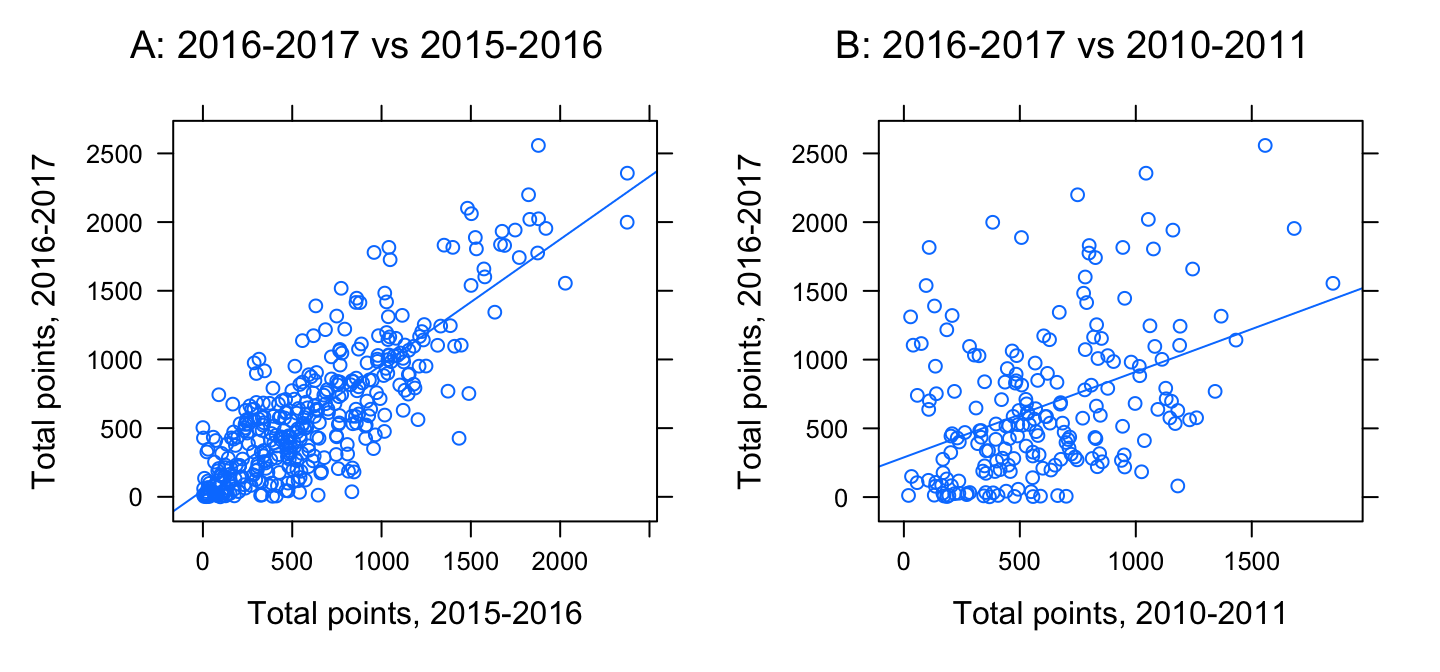
\includegraphics[width=0.49\linewidth]{08-regress_files/figure-latex/NBA-1} 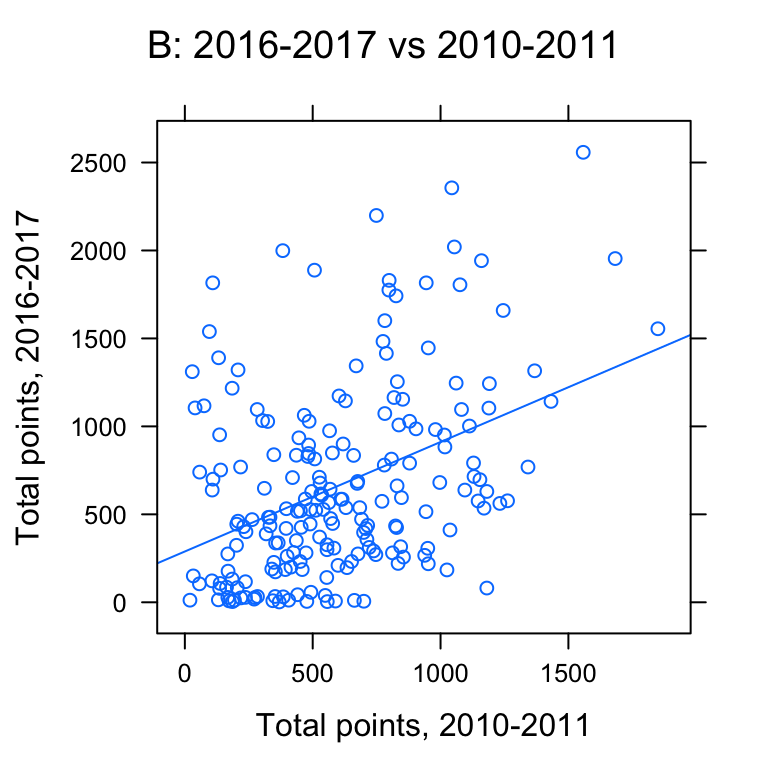
\includegraphics[width=0.49\linewidth]{08-regress_files/figure-latex/NBA-2} \caption{As time progresses, correlation decreases, and regression to the mean increases.}\label{fig:NBA}
\end{figure}

\hypertarget{the-sports-illustrated-cover-jinx}{%
\subsection*{The Sports Illustrated cover ``jinx''}\label{the-sports-illustrated-cover-jinx}}
\addcontentsline{toc}{subsection}{The Sports Illustrated cover ``jinx''}

The 21 January 2002 issue of Sports Illustrated featured an
{[}article on the so-called The Sports Illustrated cover jinx{]}
(\url{https://vault.si.com/vault/2002/01/21/that-old-black-magic-millions-of-superstitious-readersand-many-athletesbelieve-that-an-appearance-on-sports-illustrateds-cover-is-the-kiss-of-death-but-is-there-really-such-a-thing-as-the-si-jinx})\footnote{\url{https://vault.si.com/vault/2002/01/21/that-old-black-magic-millions-of-superstitious-readersand-many-athletesbelieve-that-an-appearance-on-sports-illustrateds-cover-is-the-kiss-of-death-but-is-there-really-such-a-thing-as-the-si-jinx}}
After examining covers that had appeared from 1954 to 2001, they found that

\begin{quote}
Of the 2,456 covers SI had run, 913 featured a person who, or team that,
suffered some verifiable misfortune that conformed to our definition--a Jinx
rate of 37.2\%.
\end{quote}

\href{https://en.wikipedia.org/wiki/Sports_Illustrated_cover_jinx}{Wikepedia}
has very detailed comments on the phenomenon. Especially in contact sports,
athletes who do exceptionally well will have been pushing their bodies to the
limit, with a high risk of injury.

\begin{quote}
Most athletes that seemed to suffer the jinx most typically
suffered because of an injury to their body, or some other bad
luck following their appearance.
\end{quote}

Athletes appear on the cover of a magazine such as ``Sports Illustrated''
when they are performing unusually well, both relative to their fellow
athletes, and relative to their own earlier performances. They are
likely to be approaching their peak, and/or to have experienced an
unusual run of luck. Where chance effects are the main driver,
their success is likely to be temporary, quickly dropping back to close
to or below their longer term average. Some of those who feature will
be at their peak, and will on that account soon drop back.

The Wikipedia article notes a number of athletes who went on to do
exceptionally well following appearance on the cover. Standouts
were the basketballer Michael Jordan (50 covers)~and Muhammad Ali
(40 covers). These were outstanding athletes that consistently
outperformed others.

\hypertarget{moderating-subjective-assessments}{%
\section{Moderating subjective assessments}\label{moderating-subjective-assessments}}

\begin{itemize}
\tightlist
\item
  Estimate average
\item
  Make assessment, based on what evidence seems to suggest

  \begin{itemize}
  \tightlist
  \item
    Assessment is based on current measure
  \end{itemize}
\item
  Estimate correlation between current and predicted measure.
\item
  The correlation determines the fraction of the distance
  to move from the average to the assessment.
\end{itemize}

e.g., Correlation of shotput with long jump is close to 0.4

\begin{itemize}
\tightlist
\item
  14.9 meter put is at the 93nd centile (7\% will do better)
\item
  Long jump mean = 6.97; 92\% mark 7.47 (difference=0.5)
\item
  Estimate long jump result as 6.97+0.4 \(\times\) 0.5 = 7.17
\end{itemize}

\hypertarget{forecasting-sales}{%
\subsection*{Forecasting sales}\label{forecasting-sales}}
\addcontentsline{toc}{subsection}{Forecasting sales}

You are the sales forecaster for a department store chain.\\
All stores are similar in size and merchandise offered,
but random factors affect sales in any year. Overall sales
are expected to increase by 10\% from 2020 to 2021. Sales
in 2020, with the expected total and mean for 2021 are,
in millions of dollars:

\begin{longtable}[]{@{}lll@{}}
\toprule
Store & 2020 & 2021 \\
\midrule
\endhead
1 & 10 & --- \\
2 & 23 & --- \\
3 & 18 & --- \\
4 & 29 & --- \\
TOTAL & 80 & 88 \\
MEAN & 20 & 22 \\
\bottomrule
\end{longtable}

Assuming that year to year correlation is around 0.4,
what is a reasonable estimate for sales in each of the
stores in 2021. The mean sales amount in 2021 is predicted to be 22,000,000 dollars?
With a correlation of 0.4, the predicted sales for the individual stores are
obtained thus:

\begin{longtable}[]{@{}lllll@{}}
\toprule
Store & 2020 & Subtract 20 & Xply by 0.4, add to 22 & Predicted sales \\
\midrule
\endhead
1 & 10 & -10 & 22-4 & 18 \\
2 & 23 & +3 & 22+1.2 & 23.2 \\
3 & 18 & -2 & 22-0.8 & 21.2 \\
4 & 29 & +9 & 29+3.6 & 32.6 \\
MEAN & 20 & 0 & 22 & 22 \\
\bottomrule
\end{longtable}

\hypertarget{choosing-from-job-applicants}{%
\subsection*{Choosing from job applicants}\label{choosing-from-job-applicants}}
\addcontentsline{toc}{subsection}{Choosing from job applicants}

Correlation between presentation \& performance is likely to
be lower for the less well-known. In both cases performance
is likely, relative to presentation, to move in closer to the
mean. For less well-known candidates, the shift towards the
mean is likely to~be greater.

\hypertarget{secrists-the-triumph-of-mediocrity-in-business}{%
\subsection*{Secrist's ``The Triumph of Mediocrity in Business''}\label{secrists-the-triumph-of-mediocrity-in-business}}
\addcontentsline{toc}{subsection}{Secrist's ``The Triumph of Mediocrity in Business''}

Horace Secrist's 1933 book was based on annual data for 1920 to 1930:

\begin{itemize}
\tightlist
\item
  73 different industries; examine ratios

  \begin{itemize}
  \tightlist
  \item
    Profits:sales; Profits:assets; Expenses:sales; Expenses:assets
  \end{itemize}
\item
  For each industry in 1920: split firms into 4 quartiles: top 25\%, \ldots{}

  \begin{itemize}
  \tightlist
  \item
    Took average for each statistic, for each quartile, for each year.
  \item
    Surprise, surprise, the best went, on average, down \ldots{}
  \end{itemize}
\end{itemize}

``Complete freedom to enter trade and the continuance of competition
mean the perpetuation of mediocrity. \ldots{} neither superiority or
inferiority will tend to persist. Rather, mediocrity tends to become
the rule.''

\hypertarget{note-again-regression-to-the-mean-goes-in-both-directions}{%
\subsection*{Note again --- regression to the mean goes in both directions!}\label{note-again-regression-to-the-mean-goes-in-both-directions}}
\addcontentsline{toc}{subsection}{Note again --- regression to the mean goes in both directions!}

\begin{Shaded}
\begin{Highlighting}[]
\NormalTok{cap15 }\OtherTok{\textless{}{-}} \FunctionTok{paste}\NormalTok{(}\StringTok{"Simulations based on correlation for Secrist\textquotesingle{}s data {-}{-}{-} }
\StringTok{               showing how regression to the mean goes in both directions."}\NormalTok{)}
\end{Highlighting}
\end{Shaded}

\begin{Shaded}
\begin{Highlighting}[]
\FunctionTok{par}\NormalTok{(}\AttributeTok{mfrow=}\FunctionTok{c}\NormalTok{(}\DecValTok{1}\NormalTok{,}\DecValTok{2}\NormalTok{), }\AttributeTok{mgp=}\FunctionTok{c}\NormalTok{(}\DecValTok{2}\NormalTok{,}\FloatTok{0.5}\NormalTok{,}\DecValTok{0}\NormalTok{), }\AttributeTok{mar=}\FunctionTok{c}\NormalTok{(}\FloatTok{3.1}\NormalTok{,}\FloatTok{3.1}\NormalTok{,}\FloatTok{1.6}\NormalTok{,}\FloatTok{1.1}\NormalTok{))}
\FunctionTok{set.seed}\NormalTok{(}\DecValTok{29}\NormalTok{)}
\NormalTok{x1 }\OtherTok{\textless{}{-}} \FunctionTok{rnorm}\NormalTok{(}\DecValTok{1000}\NormalTok{, }\AttributeTok{mean=}\DecValTok{34}\NormalTok{, }\AttributeTok{sd=}\DecValTok{5}\NormalTok{)}
\NormalTok{x2 }\OtherTok{\textless{}{-}} \FloatTok{0.7}\SpecialCharTok{*}\NormalTok{x1 }\SpecialCharTok{+} \FunctionTok{rnorm}\NormalTok{(}\DecValTok{1000}\NormalTok{, }\AttributeTok{mean=}\NormalTok{.}\DecValTok{3}\SpecialCharTok{*}\DecValTok{34}\NormalTok{, }\AttributeTok{sd=}\DecValTok{5}\SpecialCharTok{*}\FunctionTok{sqrt}\NormalTok{(}\DecValTok{1}\FloatTok{{-}.49}\NormalTok{))}
\NormalTok{x3 }\OtherTok{\textless{}{-}} \FloatTok{0.7}\SpecialCharTok{*}\NormalTok{x2 }\SpecialCharTok{+} \FunctionTok{rnorm}\NormalTok{(}\DecValTok{1000}\NormalTok{, }\AttributeTok{mean=}\NormalTok{.}\DecValTok{3}\SpecialCharTok{*}\DecValTok{34}\NormalTok{, }\AttributeTok{sd=}\DecValTok{5}\SpecialCharTok{*}\FunctionTok{sqrt}\NormalTok{(}\DecValTok{1}\FloatTok{{-}.49}\NormalTok{))}
\DocumentationTok{\#\# print(round(c(sd(x1),sd(x2),sd(x3)),2))}
\DocumentationTok{\#\# print(round(c(range(x1),range(x2),range(x3)),2))}
\NormalTok{xx }\OtherTok{\textless{}{-}} \FunctionTok{data.frame}\NormalTok{(}\AttributeTok{x1=}\NormalTok{x1,}\AttributeTok{x2=}\NormalTok{x2,}\AttributeTok{x3=}\NormalTok{x3)}
\NormalTok{xx }\OtherTok{\textless{}{-}}\NormalTok{ xx[}\FunctionTok{order}\NormalTok{(xx[,}\DecValTok{1}\NormalTok{]),]}
\NormalTok{qxx }\OtherTok{\textless{}{-}} \FunctionTok{sapply}\NormalTok{(xx, }\ControlFlowTok{function}\NormalTok{(x)}\FunctionTok{c}\NormalTok{(}\FunctionTok{mean}\NormalTok{(x[}\DecValTok{1}\SpecialCharTok{:}\DecValTok{250}\NormalTok{]), }\FunctionTok{mean}\NormalTok{(x[}\DecValTok{251}\SpecialCharTok{:}\DecValTok{500}\NormalTok{]),}
 \FunctionTok{mean}\NormalTok{(x[}\DecValTok{501}\SpecialCharTok{:}\DecValTok{750}\NormalTok{]),}\FunctionTok{mean}\NormalTok{(x[}\DecValTok{751}\SpecialCharTok{:}\DecValTok{1000}\NormalTok{])))}
\FunctionTok{plot}\NormalTok{(}\FunctionTok{c}\NormalTok{(}\DecValTok{1920}\NormalTok{,}\DecValTok{1925}\NormalTok{,}\DecValTok{1930}\NormalTok{),qxx[}\DecValTok{4}\NormalTok{,], }\AttributeTok{xlab=}\StringTok{""}\NormalTok{, }\AttributeTok{ylab=}\StringTok{"Profit"}\NormalTok{, }
     \AttributeTok{ylim=}\FunctionTok{c}\NormalTok{(}\FloatTok{26.6}\NormalTok{,}\FloatTok{40.7}\NormalTok{), }\AttributeTok{fg=}\StringTok{"gray"}\NormalTok{, }\AttributeTok{type=}\StringTok{"n"}\NormalTok{) }
\ControlFlowTok{for}\NormalTok{(i }\ControlFlowTok{in} \DecValTok{1}\SpecialCharTok{:}\DecValTok{4}\NormalTok{)\{}
\FunctionTok{lines}\NormalTok{(}\FunctionTok{c}\NormalTok{(}\DecValTok{1920}\NormalTok{,}\DecValTok{1925}\NormalTok{,}\DecValTok{1930}\NormalTok{),qxx[i,], }\AttributeTok{ylab=}\StringTok{"Profit"}\NormalTok{, }\AttributeTok{fg=}\StringTok{"gray"}\NormalTok{, }\AttributeTok{type=}\StringTok{"b"}\NormalTok{, }\AttributeTok{pch=}\DecValTok{16}\NormalTok{) }
\NormalTok{\}}
\FunctionTok{text}\NormalTok{(}\FunctionTok{rep}\NormalTok{(}\DecValTok{1920}\NormalTok{,}\DecValTok{4}\NormalTok{), qxx[,}\DecValTok{1}\NormalTok{], }\FunctionTok{c}\NormalTok{(}\StringTok{"Lowest 25\% in 1920"}\NormalTok{,}\StringTok{"2nd Lowest 25\% in 1920"}\NormalTok{,}
                             \StringTok{"2nd highest 25\% in 1920"}\NormalTok{, }\StringTok{"Highest 25\% in 1920"}\NormalTok{),}
     \AttributeTok{pos=}\DecValTok{4}\NormalTok{, }\AttributeTok{col=}\FunctionTok{adjustcolor}\NormalTok{(}\StringTok{"blue"}\NormalTok{,}\AttributeTok{alpha=}\FloatTok{0.5}\NormalTok{))  }
\NormalTok{xx2 }\OtherTok{\textless{}{-}}\NormalTok{ xx[}\FunctionTok{order}\NormalTok{(xx[,}\DecValTok{3}\NormalTok{]),]}
\NormalTok{qxx2 }\OtherTok{\textless{}{-}} \FunctionTok{sapply}\NormalTok{(xx2, }\ControlFlowTok{function}\NormalTok{(x)}\FunctionTok{c}\NormalTok{(}\FunctionTok{mean}\NormalTok{(x[}\DecValTok{1}\SpecialCharTok{:}\DecValTok{250}\NormalTok{]), }\FunctionTok{mean}\NormalTok{(x[}\DecValTok{251}\SpecialCharTok{:}\DecValTok{500}\NormalTok{]),}
 \FunctionTok{mean}\NormalTok{(x[}\DecValTok{501}\SpecialCharTok{:}\DecValTok{750}\NormalTok{]),}\FunctionTok{mean}\NormalTok{(x[}\DecValTok{751}\SpecialCharTok{:}\DecValTok{1000}\NormalTok{])))}
\FunctionTok{plot}\NormalTok{(}\FunctionTok{c}\NormalTok{(}\DecValTok{1920}\NormalTok{,}\DecValTok{1925}\NormalTok{,}\DecValTok{1930}\NormalTok{),qxx[}\DecValTok{4}\NormalTok{,], }\AttributeTok{xlab=}\StringTok{""}\NormalTok{, }\AttributeTok{ylab=}\StringTok{"Profit"}\NormalTok{, }
     \AttributeTok{ylim=}\FunctionTok{c}\NormalTok{(}\FloatTok{26.6}\NormalTok{,}\FloatTok{40.7}\NormalTok{), }\AttributeTok{fg=}\StringTok{"gray"}\NormalTok{, }\AttributeTok{type=}\StringTok{"n"}\NormalTok{) }
\ControlFlowTok{for}\NormalTok{(i }\ControlFlowTok{in} \DecValTok{1}\SpecialCharTok{:}\DecValTok{4}\NormalTok{)\{}
\FunctionTok{lines}\NormalTok{(}\FunctionTok{c}\NormalTok{(}\DecValTok{1920}\NormalTok{,}\DecValTok{1925}\NormalTok{,}\DecValTok{1930}\NormalTok{),qxx2[i,], }\AttributeTok{ylab=}\StringTok{"Profit"}\NormalTok{, }\AttributeTok{fg=}\StringTok{"gray"}\NormalTok{, }\AttributeTok{type=}\StringTok{"b"}\NormalTok{, }\AttributeTok{pch=}\DecValTok{16}\NormalTok{) }
\NormalTok{\}}
\FunctionTok{text}\NormalTok{(}\FunctionTok{rep}\NormalTok{(}\DecValTok{1930}\NormalTok{,}\DecValTok{4}\NormalTok{), qxx2[,}\DecValTok{3}\NormalTok{], }\FunctionTok{c}\NormalTok{(}\StringTok{"Lowest 25\% in 1930"}\NormalTok{,}\StringTok{"2nd Lowest 25\% in 1930"}\NormalTok{,}
                             \StringTok{"2nd highest 25\% in 1930"}\NormalTok{, }\StringTok{"Highest 25\% in 1930"}\NormalTok{),}
     \AttributeTok{pos=}\DecValTok{2}\NormalTok{, }\AttributeTok{col=}\FunctionTok{adjustcolor}\NormalTok{(}\StringTok{"blue"}\NormalTok{,}\AttributeTok{alpha=}\FloatTok{0.5}\NormalTok{))   }
\end{Highlighting}
\end{Shaded}

\begin{figure}[H]
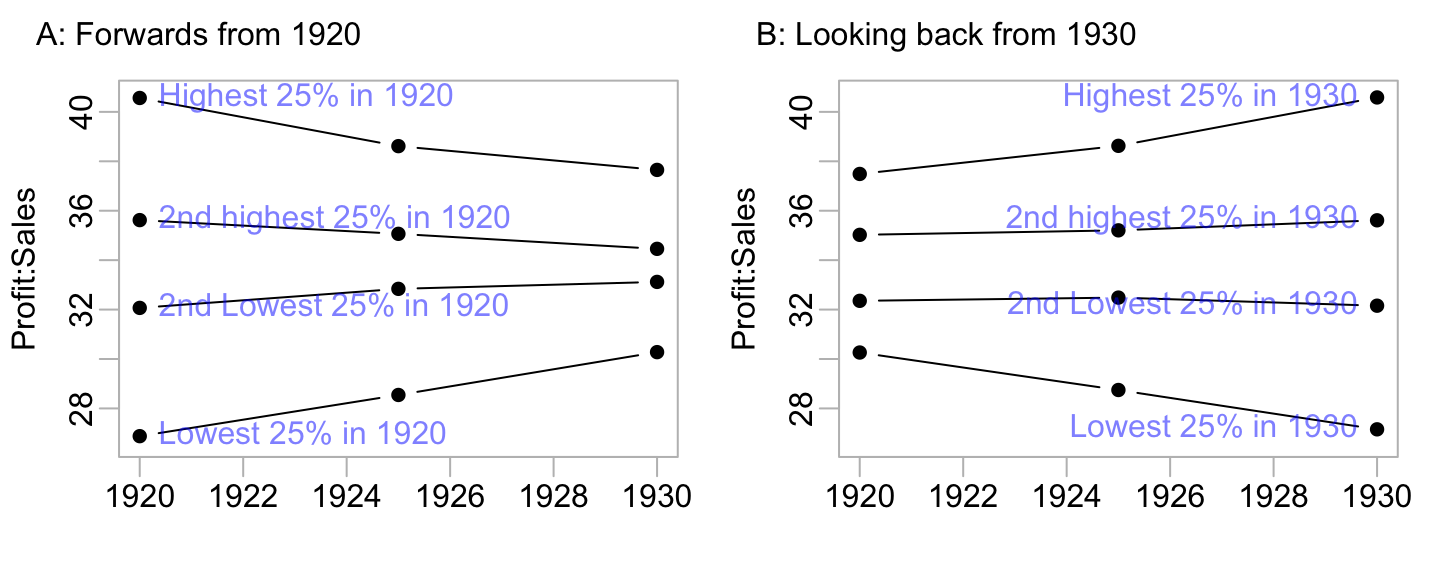
\includegraphics[width=1.05\linewidth]{08-regress_files/figure-latex/sim-1} \caption{Simulations based on correlation for Secrist's data --- 
               showing how regression to the mean goes in both directions.}\label{fig:sim}
\end{figure}

\hypertarget{do-old-fallacies-ever-die}{%
\subsection*{``Do old fallacies ever die?''}\label{do-old-fallacies-ever-die}}
\addcontentsline{toc}{subsection}{``Do old fallacies ever die?''}

Smith gives references to work by prominent economists in the past
half-century that had quoted Secrist approvingly or repeated his error.

\begin{itemize}
\tightlist
\item
  1970: ``The book {[}by Secrist{]} contains an elaborate statistical
  demonstration that, over a period of time, initially high-performing \ldots{}''
\item
  1980s investment textbook: ``Ultimately, economic forces will force
  the convergence of the profitability and growth rates of different firms.''
  This was backed up with a 1980/1966 Secrist type comparison.
\item
  2000: (Journal article) ``\ldots{} profitability is mean-reverting within
  as well as across industries. Other firms eventually mimic products
  and technologies that produce above normal profitability \ldots{}''
\item
  Friedman (2003) ``Do old fallacies ever die?'' cites other examples.
\end{itemize}

\hypertarget{covariate-adjustments-in-observational-studies}{%
\chapter{Covariate adjustments in observational studies}\label{covariate-adjustments-in-observational-studies}}

At least in principle, it is relatively straightforward to use
regression type methods to make predictions for a set of new
data that have been sampled in the same way. What is hard for
observational data, much harder than is commonly acknowledged,
is to give the model~coefficients a causal interpretation.
For this, it is necessary to have a clear understanding of the
processes involved.

\begin{itemize}
\tightlist
\item
  There will be several, perhaps a very large number,
  of explanatory variables, and an outcome variable.
\item
  The aim is to find a model that will make predictions for new data.
\item
  Note the predictive/descriptive distinction.

  \begin{itemize}
  \tightlist
  \item
    How do engineers predict building risk?
  \item
    Note the ``in sample/out of sample'' distinction.
  \item
    But is the ``new'' a random sample of the old population?\\
    (Is the `target' a random sample of the `source'?)
  \end{itemize}
\end{itemize}

There are insightful comments at:\\
\url{https://mathbabe.org/2011/06/16/the-basics-of-quantitative-modeling/}

\hypertarget{what-is-driving-predictions-sources-of-advice}{%
\section{What is driving predictions? --- sources of advice}\label{what-is-driving-predictions-sources-of-advice}}

The issues that arise for observational studies do not in general have
clear and easy answers. The discussion on
\href{https://statmodeling.stat.columbia.edu/2018/11/10/matching-discarding-non-matches-deal-lack-complete-overlap-regression-adjust-imbalance-treatment-control-groups/}{Andrew Gelman's blog}\footnote{\url{https://statmodeling.stat.columbia.edu/2018/11/10/matching-discarding-non-matches-deal-lack-complete-overlap-regression-adjust-imbalance-treatment-control-groups/}} canvasses
some of the more important issues. There are no simple answers!

Where there are several explanatory variables, and the aim is
to determine the manner in which they may be driving predictions,
matters get much~more complicated. Thus, in a comparison
between two groups (in the example that follows, midwife led
versus medical led neonatal care) one variable or factor may
be of particular interest, while other variables are used to
adjust for differences between the two groups that are at
most a secondary focus of interest. Variables that are of
secondary interest are commonly referred to as covariates.
Regression coefficients can be misleading guides to what is
driving predictions if one or more of the relevant covariates
is not available or is not properly accounted for. A paradox
of the Yule-Simpson type, sometimes referred to as Laird's
paradox, has the same potential to deceive, a potential that
should be ignored.

Little that has been published since \citet{RosBook} clarifies greatly the
advice that can be given for practical data analysis, beyond what
Rosenbaum has to say. Note, however, that \citet{pearl2018book} would
dispute this assessment. Pearl and his co-author do a good job of
highlighting important issues that should be addressed in order to
make causality judgments, at the same time overplaying what their
methodology can in general achieve. If strictly implemented,
the standards are so high that they severely limit what they can
in practice achieve. Causality diagrams have a central role.
There is a detailed, and insightful, discussion of the history
that finally led to the conclusion that smoking causes lung cancer.

\hypertarget{from-air-or-from-water-1849-deaths-from-cholera}{%
\section{From air, or from water --- 1849 deaths from cholera}\label{from-air-or-from-water-1849-deaths-from-cholera}}

Farr, who worked as statistician in the UK Registrar General's~
office, collected data on deaths from cholera in London in the
1849 epidemic. The prevailing theory at the time was that~
miasma, or bad air created~from rotting matter, was responsible
for transmitting diseases.\\
Farr classified districts into three groups this, according
to the source of the water for most of the householders:\\
1) Thames between Battersea Bridge and Waterloo Bridge, coded
as \texttt{Battersea};\\
2) New River/Rivers Lea and Ravensbourne (sources away from
the Thames), coded as \texttt{NewRiver};\\
3) Thames between Kew and Hammersmith, i.e., further up the
Thames than the first group, where the water was less polluted
by sewage, coded as \texttt{Kew}.

A regression analysis, using Farr's data, gives
results~that have been summarized in Figure \ref{fig:Farr}

\begin{figure}
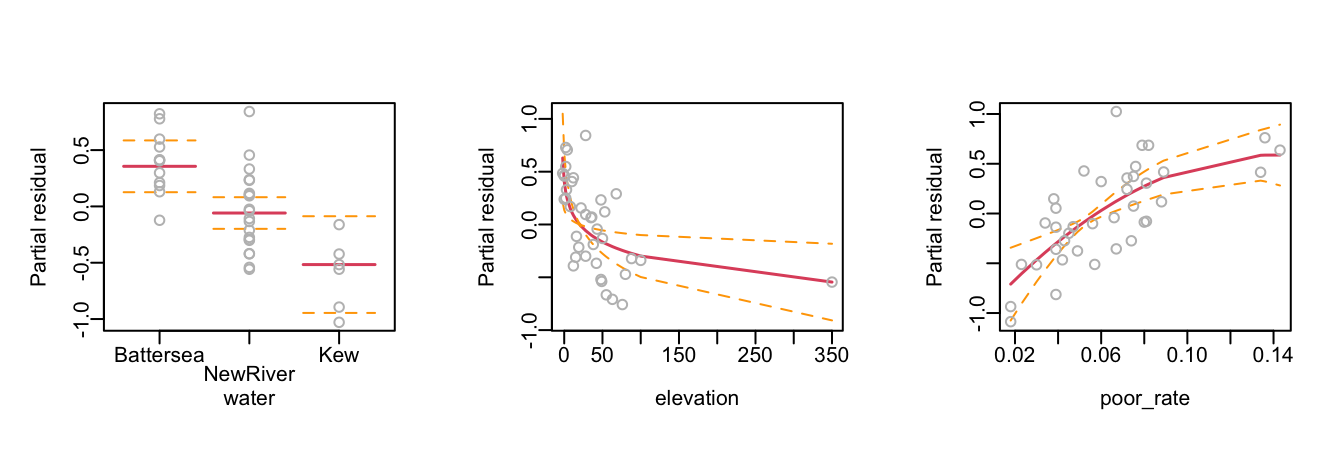
\includegraphics[width=0.32\linewidth]{09-covariate_files/figure-latex/Farr-1} 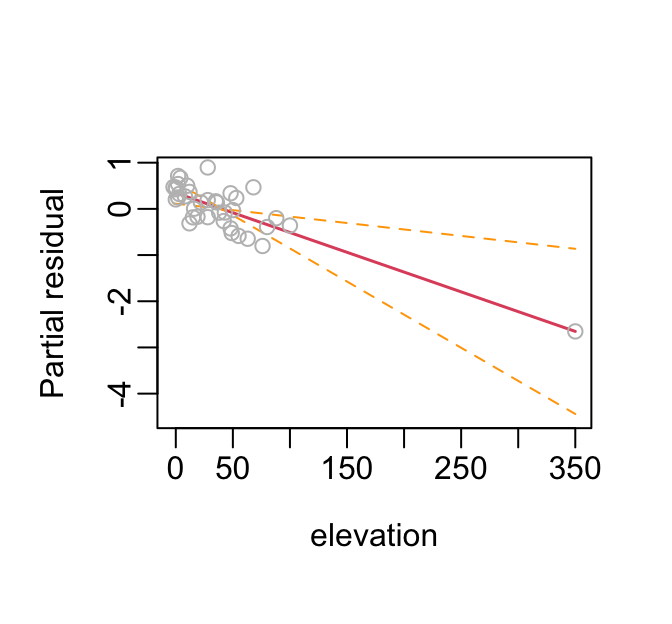
\includegraphics[width=0.32\linewidth]{09-covariate_files/figure-latex/Farr-2} 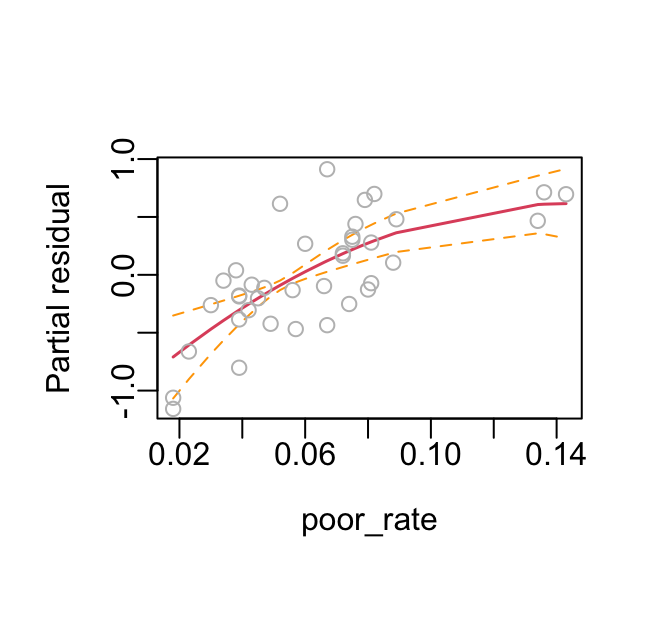
\includegraphics[width=0.32\linewidth]{09-covariate_files/figure-latex/Farr-3} \caption{Each panel shows, in turn, the estimated contribution
of a term in the model relative to the mean contribution from other 
model terms. Changes in deaths are on a `log` scale, so that an 
increase by one unit multiplies the odds of death by close to 2.7, 
around an overall mean of just over six per 1000.
}\label{fig:Farr}
\end{figure}

What can be concluded about the manner in which the three terms
contributed to death rates. None of the terms stands out as
being substantially more important than any other. Higher rates
for the poor, who were more likely to be living in crowded
conditions where it was difficult to maintain hygiene, were to
be expected.

\citet{snow1849mode} argued that those living
close to the Thames, and especially in the South, were
more likely to be getting their water from or via sources
that were likely to be contaminated with human excreta. The
piping of water up to higher ground gave contaminants
more time to settle, with less chance of exposure to human
excreta. He gave examples that he had observed directly,
where the likely means of transmission of the infection
appeared to be via a water source, or from poor hygiene.

Farr gave Snow's arguments some credibility, but discussed
ways that the air might be the main source of transmission
of an organism responsible for the disease, which multiplied
in a process akin to fermentation that was presumed to take
place in putrefying matter.

A context has to be provided in which to~interpret the data
and the regression results. While Snow had a better understanding
of the contextual information, it was not comprehensive
enough to persuade other medical specialists. Data from the
1854 epidemic, where it was possible to compare deaths supplied
from a company that continued to get its supply from lower
highly polluted Thames water with that from the company that
had moved its supply higher up to less polluted water, seems
in retrospect to~clinch the issue. The perspective brought by
germ theory would come later, with the work of Pasteur in the
late 1850s and Koch in the 1880s.

\hypertarget{are-there-missing-covariates}{%
\section{Are there missing covariates?}\label{are-there-missing-covariates}}

The \citep{wernham_EtAl_2016} study used data from 244,047 singleton term
deliveries that occurred between 2008 and 2012. It made the claim
that midwife led care, as opposed to medical led care, gave a
greater risk of adverse fetal and neonatal outcomes. Notably, the
claim was that midwife led care resulted in a lower Apgar score
(a measure of infant health immediately after birth) and a greater
risk of the imprecisely defined diagnosis of birth asphyxia.
Studies that are similarly relatively carefully done,
but naive in the weight placed on the regression results,
are embarrassingly common.

This study was then the basis for exaggerated claims in an article
in the October 8-14 2016 issue of the NZ
Listener \citep[ ``Birth Control'']{chisholm_2016}. Contrary to what was
claimed, the research did not
``lob a grenade into the historically war-torn territory of
New Zealand's maternity care.''
Even less did its results warrant the melodramatic claims of
``Alarming maternity research'' and ``Revolution gone wrong'' that
appeared on the Listener's front cover.

A major~issue with the analysis is that it relies on using
the {[}NZ Deprivation Index{]}
(\url{https://www.health.govt.nz/publication/nzdep2013-index-deprivation})
to adjust for socioeconomic differences. This provides a deprivation
score for meshblocks, each of around 60--110 people. It estimates the
relative socioeconomic deprivation of an area, and does not directly
relate to individuals. Deprived areas will often include some
individuals with high socioeconomic status. Caesarean section, as a
delivery type, may well have been more accessible for those of
higher socioeconomic status. For National Women's in Auckland,
the elective Caesarean rate at term over 2006-2015 for doctor-led
care was 32.8\%, as against 7.4\% for self employed midwives
{[}farquhar2016letter{]}. Effects from fetal alcohol syndrome were
not accounted for, nor were direct effects from substance abuse.
According to NZ Ministry of Health information, international data
indicates that
{[}fetal alcohol syndrome may affect as many as 3\% of births{]}
(\url{https://www.health.govt.nz/our-work/diseases-and-conditions/fetal-alcohol-spectrum-disorder})

There are analysis tools, and associated graphs, that the authors
of the study could and should have used to shed light on the likely
effectiveness of the covariate adjustments.

\hypertarget{sec:lancet}{%
\section{The May 2020 Lancet paper that was quickly withdrawn}\label{sec:lancet}}

Thirteen days after it was published on May 20 2020, three of the
four authors withdrew a paper that claimed to~find that malaria drugs,
when used experimentally with patients with Covid-19, led to around
30\% excess deaths. Irrespective of the problems with the data that
will be noted shortly, serious flaws in the analysis ought to~have
attracted the attention of referees. There was inadequate
adjustment for known and measured confounders (disease severity,
temporal effects, site effects, dose used).

The study claimed to~be based on data from 96,032
hospitalized COVID-19 patients from six continents, of which 66\%
were from North Ammerica. Very soon after it appeared, the article
attracted critical attention, with a number of critics joining
together to submit the letter \citet{watson2020open} to Lancet.

The sources from which the data had been obtained could not be verified,
data that claimed to be from just five Australian sources had more
cases than the total of Australian government figures, and similarly
for Australian deaths, there were implausibly small reported variances
in baseline variables, mean daily doses of hydroxychloroquine that were
100 mg higher than US FDA recommendations.

Randomized trials designed to test the effectiveness of the drugs,
and that were in progress at the time when the paper appeared,
were temporarily halted. The eventual~conclusion was that the
drugs did not improve medical outcomes. There was some evidence
that hydroxychloroquine could have adverse effects.

With current web-based technology, RCTs can be planned and carried out and yield definitive answers, in much the same time as it would take to collect and analyze the data that are required for an observational study whose conclusions can be, at best, suggestive. Data confidentiality issues are easier to handle in the context of an RCT.

\hypertarget{the-uses-and-traps-of-algorithmic-methods-trees}{%
\section{The uses and traps of ``algorithmic'' methods -- trees}\label{the-uses-and-traps-of-algorithmic-methods-trees}}

Take as an example spam prediction, using tree-based methods.
The boxplots in the figure show the distributions of variable
values.

\begin{Shaded}
\begin{Highlighting}[]
\NormalTok{cap16 }\OtherTok{\textless{}{-}} \FunctionTok{paste}\NormalTok{(}\StringTok{"Boxplots, showing distribution of variable values}
\StringTok{               in data used to predict email spam"}\NormalTok{)}
\end{Highlighting}
\end{Shaded}

\begin{Shaded}
\begin{Highlighting}[]
\FunctionTok{par}\NormalTok{(}\AttributeTok{oma=}\FunctionTok{c}\NormalTok{(}\DecValTok{0}\NormalTok{,}\DecValTok{3}\NormalTok{,}\DecValTok{0}\NormalTok{,}\DecValTok{0}\NormalTok{), }\AttributeTok{mfrow=}\FunctionTok{c}\NormalTok{(}\DecValTok{2}\NormalTok{,}\DecValTok{6}\NormalTok{), }\AttributeTok{mgp=}\FunctionTok{c}\NormalTok{(}\DecValTok{1}\NormalTok{,}\FloatTok{0.5}\NormalTok{,}\DecValTok{0}\NormalTok{), }\AttributeTok{mar=}\FunctionTok{c}\NormalTok{(}\FloatTok{3.1}\NormalTok{,}\FloatTok{3.6}\NormalTok{,}\FloatTok{1.6}\NormalTok{,.}\DecValTok{6}\NormalTok{),}\AttributeTok{las=}\DecValTok{0}\NormalTok{)}
\NormalTok{nam }\OtherTok{\textless{}{-}} \FunctionTok{c}\NormalTok{(}\StringTok{"crl.tot"}\NormalTok{, }\StringTok{"dollar"}\NormalTok{, }\StringTok{"bang"}\NormalTok{, }\StringTok{"money"}\NormalTok{, }\StringTok{"n000"}\NormalTok{, }\StringTok{"make"}\NormalTok{)}
\NormalTok{  nr }\OtherTok{\textless{}{-}} \FunctionTok{sample}\NormalTok{(}\DecValTok{1}\SpecialCharTok{:}\FunctionTok{dim}\NormalTok{(DAAG}\SpecialCharTok{::}\NormalTok{spam7)[}\DecValTok{1}\NormalTok{],}\DecValTok{500}\NormalTok{)}
\NormalTok{  yesno}\OtherTok{\textless{}{-}}\NormalTok{DAAG}\SpecialCharTok{::}\NormalTok{spam7}\SpecialCharTok{$}\NormalTok{yesno[nr]}
\NormalTok{  spam7 }\OtherTok{\textless{}{-}}\NormalTok{ DAAG}\SpecialCharTok{::}\NormalTok{spam7[nr,nam]}
\NormalTok{  nam2 }\OtherTok{\textless{}{-}} \FunctionTok{names}\NormalTok{(spam7)}
\NormalTok{  nam2[}\DecValTok{1}\NormalTok{] }\OtherTok{\textless{}{-}} \StringTok{"Total runs of capitals"}  
\NormalTok{  nam2[}\DecValTok{2}\NormalTok{] }\OtherTok{\textless{}{-}} \StringTok{"No. of \textquotesingle{}$\textquotesingle{} as \% of symbols"}
\NormalTok{  nam2[}\DecValTok{3}\NormalTok{] }\OtherTok{\textless{}{-}} \StringTok{"No. \textquotesingle{}!\textquotesingle{} as \% of symbols"}
\NormalTok{  nam2[}\DecValTok{4}\NormalTok{] }\OtherTok{\textless{}{-}} \StringTok{"No. \textquotesingle{}money\textquotesingle{}, as \% of words"}  
\NormalTok{  nam2[}\DecValTok{5}\NormalTok{] }\OtherTok{\textless{}{-}} \StringTok{"No. \textquotesingle{}make\textquotesingle{}, as \% of words"}
\NormalTok{  nam2[}\DecValTok{6}\NormalTok{] }\OtherTok{\textless{}{-}} \StringTok{"No. \textquotesingle{}000\textquotesingle{}, as \% of words"}
\NormalTok{  spam7}\FloatTok{.2} \OtherTok{\textless{}{-}}\NormalTok{ spam7}
\NormalTok{  spam7}\FloatTok{.2}\NormalTok{[,}\DecValTok{1}\NormalTok{]}\OtherTok{\textless{}{-}}\FunctionTok{log}\NormalTok{(spam7}\FloatTok{.2}\NormalTok{[,}\DecValTok{1}\NormalTok{]}\SpecialCharTok{+}\FloatTok{0.5}\NormalTok{)}
\NormalTok{  spam7}\FloatTok{.2}\NormalTok{[,}\DecValTok{2}\SpecialCharTok{:}\DecValTok{6}\NormalTok{]}\OtherTok{\textless{}{-}}\FunctionTok{log}\NormalTok{(spam7}\FloatTok{.2}\NormalTok{[,}\DecValTok{2}\SpecialCharTok{:}\DecValTok{6}\NormalTok{]}\SpecialCharTok{+}\FloatTok{0.5}\NormalTok{)}
  \ControlFlowTok{for}\NormalTok{ (namtxt }\ControlFlowTok{in}\NormalTok{ nam)\{}
    \FunctionTok{boxplot}\NormalTok{(}\FunctionTok{split}\NormalTok{(spam7[,namtxt],yesno),}\AttributeTok{cex=}\FloatTok{0.65}\NormalTok{,}\AttributeTok{axes=}\NormalTok{F,}\AttributeTok{boxwex=}\FloatTok{0.5}\NormalTok{)}
    \FunctionTok{box}\NormalTok{()}
    \FunctionTok{par}\NormalTok{(}\AttributeTok{mgp=}\FunctionTok{c}\NormalTok{(}\DecValTok{1}\NormalTok{,.}\DecValTok{5}\NormalTok{,}\DecValTok{0}\NormalTok{))}
    \FunctionTok{axis}\NormalTok{(}\DecValTok{2}\NormalTok{, }\AttributeTok{cex.axis=}\DecValTok{1}\NormalTok{)}
    \FunctionTok{par}\NormalTok{(}\AttributeTok{mgp=}\FunctionTok{c}\NormalTok{(}\DecValTok{1}\NormalTok{,.}\DecValTok{25}\NormalTok{,}\DecValTok{0}\NormalTok{))}
    \FunctionTok{axis}\NormalTok{(}\DecValTok{1}\NormalTok{,}\AttributeTok{at=}\DecValTok{1}\SpecialCharTok{:}\DecValTok{2}\NormalTok{,}\AttributeTok{labels=}\FunctionTok{c}\NormalTok{(}\StringTok{"n"}\NormalTok{,}\StringTok{"y"}\NormalTok{))}
\NormalTok{    i }\OtherTok{\textless{}{-}} \FunctionTok{match}\NormalTok{(namtxt,nam)}
    \FunctionTok{mtext}\NormalTok{(}\AttributeTok{side=}\DecValTok{2}\NormalTok{,}\AttributeTok{line=}\FloatTok{1.75}\NormalTok{,nam2[i],}\AttributeTok{adj=}\FloatTok{0.5}\NormalTok{,}\AttributeTok{cex=}\FloatTok{0.8}\NormalTok{)}
\NormalTok{  \}}
\NormalTok{  xval }\OtherTok{\textless{}{-}}\FunctionTok{c}\NormalTok{(.}\DecValTok{1}\NormalTok{,.}\DecValTok{2}\NormalTok{,.}\DecValTok{5}\NormalTok{,}\DecValTok{1}\NormalTok{,}\DecValTok{2}\NormalTok{,}\DecValTok{5}\NormalTok{,}\DecValTok{10}\NormalTok{,}\DecValTok{20}\NormalTok{,}\DecValTok{50}\NormalTok{,}\DecValTok{100}\NormalTok{,}\DecValTok{200}\NormalTok{,}\DecValTok{500}\NormalTok{,}\DecValTok{1000}\NormalTok{,}\DecValTok{2000}\NormalTok{)}
  \ControlFlowTok{for}\NormalTok{ (namtxt }\ControlFlowTok{in}\NormalTok{ nam)\{}
    \FunctionTok{boxplot}\NormalTok{(}\FunctionTok{split}\NormalTok{(spam7}\FloatTok{.2}\NormalTok{[,namtxt],yesno),}\AttributeTok{cex=}\FloatTok{0.65}\NormalTok{,}\AttributeTok{axes=}\NormalTok{F,}\AttributeTok{boxwex=}\FloatTok{0.5}\NormalTok{)}
    \FunctionTok{box}\NormalTok{()}
\NormalTok{    ranx }\OtherTok{\textless{}{-}} \FunctionTok{range}\NormalTok{(spam7[,namtxt])}
\NormalTok{    yloc}\OtherTok{\textless{}{-}}\NormalTok{xval[xval}\SpecialCharTok{\textgreater{}=}\FunctionTok{min}\NormalTok{(ranx)}\SpecialCharTok{\&}\NormalTok{xval}\SpecialCharTok{\textless{}}\FunctionTok{max}\NormalTok{(ranx)]}
    \FunctionTok{par}\NormalTok{(}\AttributeTok{mgp=}\FunctionTok{c}\NormalTok{(}\DecValTok{1}\NormalTok{,.}\DecValTok{5}\NormalTok{,}\DecValTok{0}\NormalTok{))}
    \FunctionTok{axis}\NormalTok{(}\DecValTok{2}\NormalTok{,}\AttributeTok{at=}\FunctionTok{log}\NormalTok{(yloc}\FloatTok{+0.5}\NormalTok{),}\AttributeTok{labels=}\FunctionTok{paste}\NormalTok{(}\FunctionTok{round}\NormalTok{(yloc,}\DecValTok{1}\NormalTok{)), }\AttributeTok{cex.axis=}\DecValTok{1}\NormalTok{)}
    \FunctionTok{par}\NormalTok{(}\AttributeTok{mgp=}\FunctionTok{c}\NormalTok{(}\DecValTok{1}\NormalTok{,.}\DecValTok{25}\NormalTok{,}\DecValTok{0}\NormalTok{))}
    \FunctionTok{axis}\NormalTok{(}\DecValTok{1}\NormalTok{,}\AttributeTok{at=}\DecValTok{1}\SpecialCharTok{:}\DecValTok{2}\NormalTok{,}\AttributeTok{labels=}\FunctionTok{c}\NormalTok{(}\StringTok{"n"}\NormalTok{,}\StringTok{"y"}\NormalTok{))}
\NormalTok{    i }\OtherTok{\textless{}{-}} \FunctionTok{match}\NormalTok{(namtxt,nam)}
    \ControlFlowTok{if}\NormalTok{(i}\SpecialCharTok{==}\DecValTok{1}\NormalTok{)}\FunctionTok{mtext}\NormalTok{(}\AttributeTok{side=}\DecValTok{2}\NormalTok{,}\AttributeTok{line=}\DecValTok{1}\NormalTok{,}\StringTok{"(Logarithmic scales)"}\NormalTok{,}\AttributeTok{outer=}\NormalTok{T,}\AttributeTok{at=}\FloatTok{0.25}\NormalTok{)}
    \FunctionTok{mtext}\NormalTok{(}\AttributeTok{side=}\DecValTok{2}\NormalTok{,}\AttributeTok{line=}\FloatTok{1.75}\NormalTok{,nam2[i],}\AttributeTok{adj=}\FloatTok{0.5}\NormalTok{,}\AttributeTok{cex=}\FloatTok{0.8}\NormalTok{)}
\NormalTok{  \}}
\end{Highlighting}
\end{Shaded}

\begin{figure}
\centering
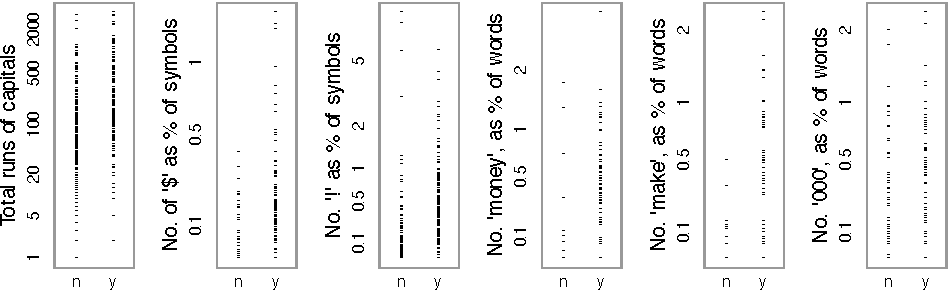
\includegraphics{09-covariate_files/figure-latex/seeSpam-1.pdf}
\caption{\label{fig:seeSpam}Boxplots, showing distribution of variable values
in data used to predict email spam}
\end{figure}

The decision tree that is obtained is:

\begin{Shaded}
\begin{Highlighting}[]
\NormalTok{cap17 }\OtherTok{\textless{}{-}} \FunctionTok{paste}\NormalTok{(}\StringTok{"Decision tree for spam data. If the condition is satisfied, take}
\StringTok{               the branch to the left.  Otherwise, take the branch to the right."}\NormalTok{)}
\end{Highlighting}
\end{Shaded}

\begin{Shaded}
\begin{Highlighting}[]
\FunctionTok{par}\NormalTok{(}\AttributeTok{mar=}\FunctionTok{c}\NormalTok{(}\FloatTok{4.1}\NormalTok{,}\FloatTok{3.1}\NormalTok{,}\FloatTok{2.6}\NormalTok{,}\FloatTok{0.6}\NormalTok{), }\AttributeTok{xpd=}\ConstantTok{TRUE}\NormalTok{)}
\FunctionTok{require}\NormalTok{(rpart)}
\NormalTok{spam.rpart }\OtherTok{\textless{}{-}} \FunctionTok{rpart}\NormalTok{(}\AttributeTok{formula =}\NormalTok{ yesno }\SpecialCharTok{\textasciitilde{}}\NormalTok{ crl.tot }\SpecialCharTok{+}\NormalTok{ dollar }\SpecialCharTok{+}\NormalTok{ bang }\SpecialCharTok{+}
\NormalTok{   money }\SpecialCharTok{+}\NormalTok{ n000 }\SpecialCharTok{+}\NormalTok{ make, }\AttributeTok{data=}\NormalTok{DAAG}\SpecialCharTok{::}\NormalTok{spam7)}
\FunctionTok{plot}\NormalTok{(spam.rpart, }\AttributeTok{uniform=}\ConstantTok{TRUE}\NormalTok{)}
\FunctionTok{text}\NormalTok{(spam.rpart)}
\FunctionTok{par}\NormalTok{(}\AttributeTok{mar=}\FunctionTok{c}\NormalTok{(}\DecValTok{0}\NormalTok{,}\DecValTok{4}\NormalTok{,}\DecValTok{0}\NormalTok{,}\DecValTok{0}\NormalTok{))}
\FunctionTok{plot}\NormalTok{(}\FunctionTok{c}\NormalTok{(}\DecValTok{1}\NormalTok{,}\DecValTok{8}\NormalTok{),}\FunctionTok{c}\NormalTok{(}\FloatTok{0.5}\NormalTok{,}\FloatTok{8.5}\NormalTok{), }\AttributeTok{asp=}\FloatTok{0.4}\NormalTok{, }\AttributeTok{axes=}\ConstantTok{FALSE}\NormalTok{, }\AttributeTok{type=}\StringTok{"n"}\NormalTok{, }\AttributeTok{bty=}\StringTok{"n"}\NormalTok{, }\AttributeTok{cex=}\FloatTok{0.8}\NormalTok{, }\AttributeTok{xlab=}\StringTok{""}\NormalTok{,}\AttributeTok{ylab=}\StringTok{""}\NormalTok{)}
\FunctionTok{text}\NormalTok{(}\DecValTok{1}\NormalTok{,}\FloatTok{8.0}\NormalTok{, }\StringTok{"  "}\NormalTok{,}\AttributeTok{pos=}\DecValTok{4}\NormalTok{)}
\FunctionTok{text}\NormalTok{(}\DecValTok{2}\NormalTok{,}\FloatTok{8.0}\NormalTok{, }\StringTok{"Symbols used in tree are:"}\NormalTok{,}\AttributeTok{pos=}\DecValTok{4}\NormalTok{)}
\FunctionTok{text}\NormalTok{(}\DecValTok{2}\NormalTok{,}\FloatTok{6.0}\NormalTok{, }\StringTok{"dollar: Number of \textasciigrave{}$\textasciigrave{} symbols}\SpecialCharTok{\textbackslash{}n}\StringTok{(as \% of symbols)"}\NormalTok{,}\AttributeTok{pos=}\DecValTok{4}\NormalTok{)}
\FunctionTok{text}\NormalTok{(}\DecValTok{2}\NormalTok{,}\FloatTok{3.5}\NormalTok{, }\StringTok{"bang: Number of \textasciigrave{}!\textasciigrave{} symbols}\SpecialCharTok{\textbackslash{}n}\StringTok{(as \% of symbols)"}\NormalTok{,}\AttributeTok{pos=}\DecValTok{4}\NormalTok{)}
\FunctionTok{text}\NormalTok{(}\DecValTok{2}\NormalTok{,}\FloatTok{1.5}\NormalTok{, }\StringTok{"crl.tot: Total runs of capitals"}\NormalTok{,}\AttributeTok{pos=}\DecValTok{4}\NormalTok{)}
\FunctionTok{text}\NormalTok{(}\DecValTok{2}\NormalTok{,}\FloatTok{0.75}\NormalTok{, }\StringTok{"  "}\NormalTok{, }\AttributeTok{pos=}\DecValTok{4}\NormalTok{)}
\end{Highlighting}
\end{Shaded}

\begin{figure}[H]
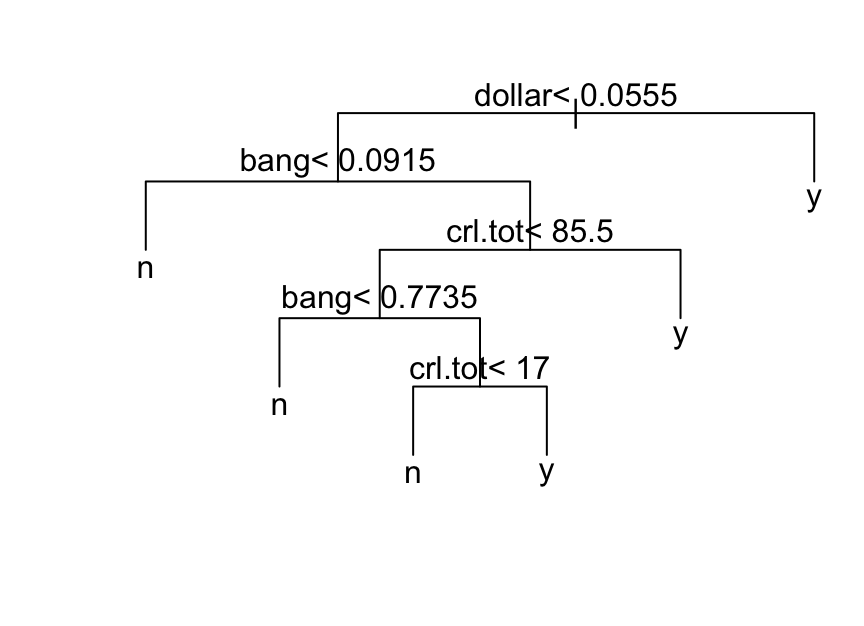
\includegraphics[width=0.48\linewidth]{09-covariate_files/figure-latex/spam-1} 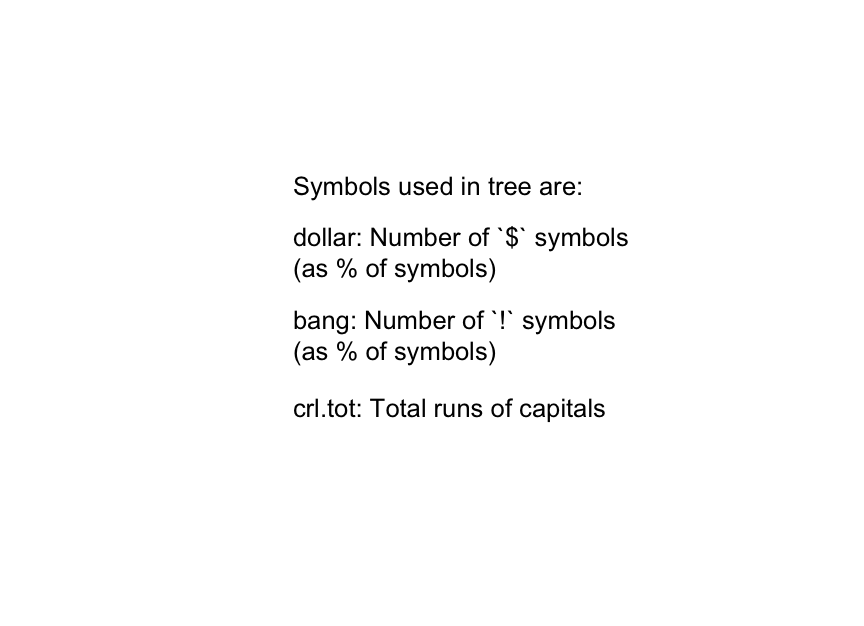
\includegraphics[width=0.48\linewidth]{09-covariate_files/figure-latex/spam-2} \caption{Decision tree for spam data. If the condition is satisfied, take
               the branch to the left.  Otherwise, take the branch to the right.}\label{fig:spam}
\end{figure}

\hypertarget{from-trees-to-forests}{%
\subsection*{From trees to forests}\label{from-trees-to-forests}}
\addcontentsline{toc}{subsection}{From trees to forests}

Trees such as shown will often have poor predictive power.
A much more effective way to use ``trees'', in many or most
cases, is to make a forest (a ``random forest''), and then
vote between the trees. A downside is that ``Random forests''
and similar methods operate largely as black boxes.

\begin{itemize}
\tightlist
\item
  Random forest type methods may work well when the way that
  explanatory factors conspire to give an output is unclear.
\item
  What works, but one does not know why, may be effective for
  present circumstances.
\item
  This can be both a trap and a virtue. Thus, for detecting spam:

  \begin{itemize}
  \tightlist
  \item
    When it fails, we will likely have few clues why!
  \item
    This may, for a short time, impede spammers!
  \end{itemize}
\item
  Spammers are anyway continually refining their strategies

  \begin{itemize}
  \tightlist
  \item
    Spam detectors must be responsive to new challenges
  \end{itemize}
\item
  Automated systems that can be easily gamed abound. They are a
  menace!
\end{itemize}

\hypertarget{it-helps-to-know-the-how-and-why-of-the-algorithms-used}{%
\subsection*{It helps to know the how and why of the algorithms used}\label{it-helps-to-know-the-how-and-why-of-the-algorithms-used}}
\addcontentsline{toc}{subsection}{It helps to know the how and why of the algorithms used}

Cathy O'Neill: ``\ldots{} it's not enough to just know how to run a black box
algorithm. You actually need to know how and why it works, so that when
it does'nt work, you can adjust.''

\hypertarget{regression-bloopers-examples-of-other-traps}{%
\section{Regression bloopers -- examples of other traps}\label{regression-bloopers-examples-of-other-traps}}

\vspace*{-5pt}

\hypertarget{herricanes-vs-himmicanes}{%
\subsection*{Herricanes vs Himmicanes}\label{herricanes-vs-himmicanes}}
\addcontentsline{toc}{subsection}{Herricanes vs Himmicanes}

\begin{Shaded}
\begin{Highlighting}[]
\NormalTok{cap18 }\OtherTok{\textless{}{-}} \StringTok{"Deaths versus damage estimate in US dollars, with logarithmic scales}
\StringTok{               on both axes. Separate fitted lines for male and female}
\StringTok{               hurricanes cannot be distinguished. Jung et al used a }
\StringTok{               logarithmic scale on the vertical axis only, which on}
\StringTok{               this graph leads to the dashed curves."}
\end{Highlighting}
\end{Shaded}

\begin{figure}
\centering
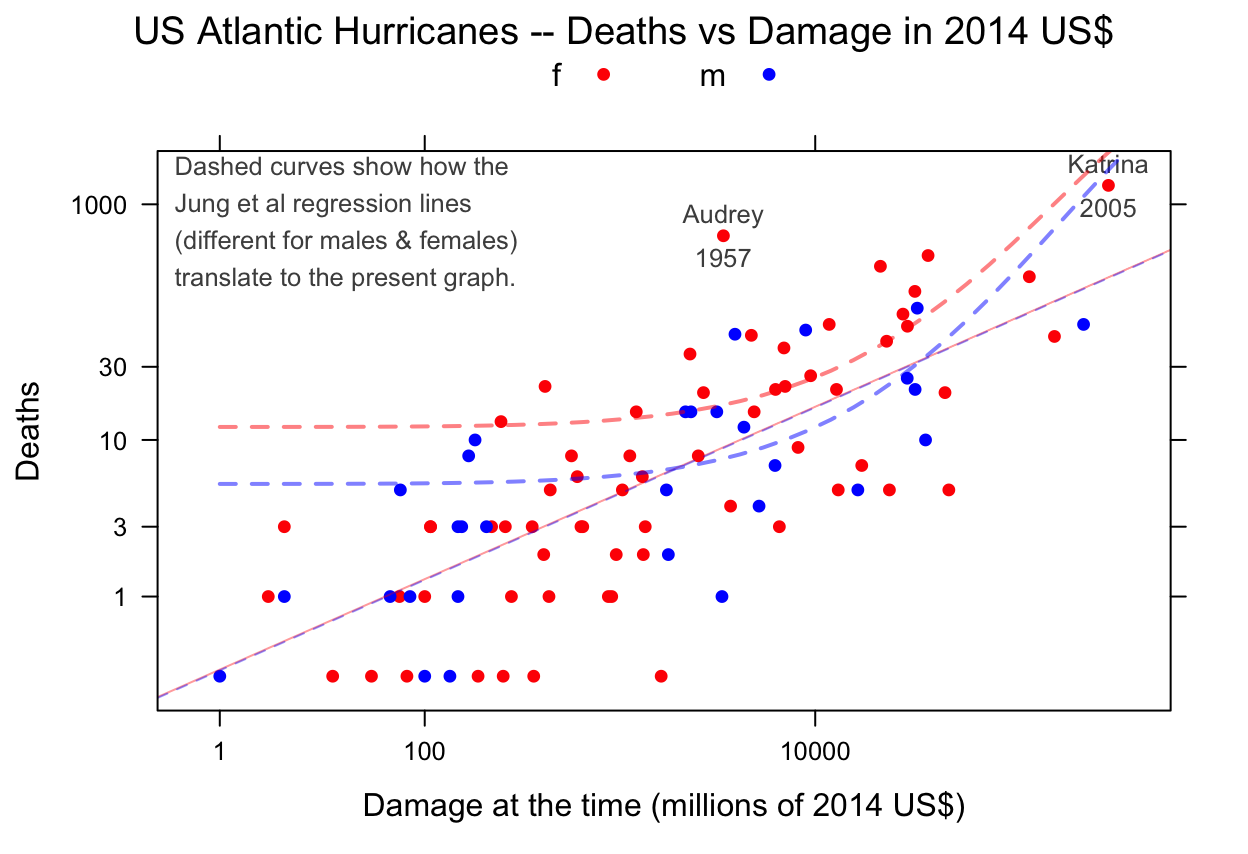
\includegraphics{09-covariate_files/figure-latex/hurricanes-1.pdf}
\caption{\label{fig:hurricanes}Deaths versus damage estimate in US dollars, with logarithmic scales
on both axes. Separate fitted lines for male and female
hurricanes cannot be distinguished. Jung et al used a
logarithmic scale on the vertical axis only, which on
this graph leads to the dashed curves.}
\end{figure}

Authors of a paper titled ``Female hurricanes are deadlier than male
hurricanes'' \citep{jung2014female} compared death rates from hurricanes
with female names with death rates for those given male names
(jokingly called himmicanes), for 94 Atlantic hurricanes that made
landfall in the United States during 1950-2012. The suggestion was
that authorities took the risk from hurricanes with female names
less seriously. A storm of reaction on the blogosphere was mostly
himmicane!

As the primary measure of the
risk posed by the hurricanes, the authors used a 2013 US\$ estimate
of damage that could have been expected from a comparable hurricane
in 2013. Figure \ref{fig:hurricanes} uses, instead, the estimate of
damage at the time, converted to 2014 US\$.

The Jung et al analysis was roughly equivalent to regressing
\(\log\)(\mbox{deaths}) on a their 2013 US\$ measure of damage,
accounting also for femaleness of the name, a minor effect from
barometric pressure at landfall, and interactions. Why did the
authors not use, at least as a starting point, the same
transformation on both axes, as in Figure \ref{fig:hurricanes}?
The femaleness effect then vanishes.

Jung et al's damage measure, because designed for use for 2013
insurance purposes, assessed risk to the infrastructure
that was in place in 2013. The damage measure that is
more relevant to risk to human life at the time is damage caused at
the time, in inflation-adjusted dollars. This makes little
difference to the graph or to the analysis.

Yet another issue was that the judgment on how female a name sounded
was~made by students in 2014. Unconscious judgments that might have
influenced disaster management, at the time when the hurricanes occurred,
would very likely have been different.

\hypertarget{historical-speed-of-light-estimates-is-there-a-pattern}{%
\subsection*{Historical speed of light estimates --- is there a pattern?}\label{historical-speed-of-light-estimates-is-there-a-pattern}}
\addcontentsline{toc}{subsection}{Historical speed of light estimates --- is there a pattern?}

Creationist Barry Setterfield has argued that a reduction over time
in the speed of light has led the passage of time to slow down,
relative to the remote past, so that the universe is thousands
rather than billions of years old. His arguments rely on
making various adjustments to figures obtained historically,
selecting what he regarded as the most reliable data, and
then fitting a curve. He tells a story that is very different
from that of Panel A of Figure \ref{fig:plot-c-data}.
Data are from \url{https://en.wikipedia.org/wiki/Speed_of_light}.

\begin{Shaded}
\begin{Highlighting}[]
\NormalTok{cvalues }\OtherTok{\textless{}{-}} \FunctionTok{data.frame}\NormalTok{(}
  \AttributeTok{Year =} \FunctionTok{c}\NormalTok{(}\DecValTok{1675}\NormalTok{, }\DecValTok{1729}\NormalTok{, }\DecValTok{1849}\NormalTok{, }\DecValTok{1862}\NormalTok{, }\DecValTok{1907}\NormalTok{, }\DecValTok{1926}\NormalTok{, }\DecValTok{1950}\NormalTok{, }\DecValTok{1958}\NormalTok{, }\DecValTok{1972}\NormalTok{),}
  \AttributeTok{speed =} \FunctionTok{c}\NormalTok{(}\DecValTok{220000}\NormalTok{, }\DecValTok{301000}\NormalTok{, }\DecValTok{315000}\NormalTok{, }\DecValTok{298000}\NormalTok{, }\DecValTok{299710}\NormalTok{, }\DecValTok{299796}\NormalTok{,}
            \FloatTok{299792.5}\NormalTok{, }\FloatTok{299792.50}\NormalTok{, }\FloatTok{299792.4562}\NormalTok{)}\SpecialCharTok{/}\DecValTok{1000}\NormalTok{,}
  \AttributeTok{error =} \FunctionTok{c}\NormalTok{(}\ConstantTok{NA}\NormalTok{, }\ConstantTok{NA}\NormalTok{, }\ConstantTok{NA}\NormalTok{, }\DecValTok{500}\NormalTok{, }\DecValTok{30}\NormalTok{, }\DecValTok{4}\NormalTok{, }\DecValTok{3}\NormalTok{, }\FloatTok{0.1}\NormalTok{, }\FloatTok{0.00111}\NormalTok{)}\SpecialCharTok{/}\DecValTok{1000}
\NormalTok{)}
\end{Highlighting}
\end{Shaded}

\begin{Shaded}
\begin{Highlighting}[]
\NormalTok{cap19 }\OtherTok{\textless{}{-}} \StringTok{"Successive speed of light estimates.}
\StringTok{Error estimates are available for the 1855 and later}
\StringTok{measurments.  Panel B limits attention to measurements}
\StringTok{made in 1926 and later. The line }
\StringTok{was fitted with no adjustment for the very different error}
\StringTok{estimates.  The dashed curve, which incorporates}
\StringTok{such adjustments, is statistically indistinguishable}
\StringTok{from the red horizontal line."}
\end{Highlighting}
\end{Shaded}

\begin{Shaded}
\begin{Highlighting}[]
\FunctionTok{par}\NormalTok{(}\AttributeTok{mfrow=}\FunctionTok{c}\NormalTok{(}\DecValTok{1}\NormalTok{,}\DecValTok{2}\NormalTok{), }\AttributeTok{mar=}\FunctionTok{c}\NormalTok{(}\FloatTok{3.1}\NormalTok{,}\FloatTok{4.1}\NormalTok{,}\FloatTok{2.1}\NormalTok{,}\FloatTok{0.6}\NormalTok{))}
\FunctionTok{plot}\NormalTok{(speed }\SpecialCharTok{\textasciitilde{}}\NormalTok{ Year, }\AttributeTok{data=}\NormalTok{cvalues, }\AttributeTok{cex=}\FloatTok{1.0}\NormalTok{, }\AttributeTok{cex.lab=}\FloatTok{1.0}\NormalTok{, }\AttributeTok{pch=}\DecValTok{1}\NormalTok{,}
     \AttributeTok{xlab=}\StringTok{""}\NormalTok{, }\AttributeTok{ylab=}\StringTok{"Speed (1000s of km/s)"}\NormalTok{)}
\FunctionTok{rect}\NormalTok{(}\DecValTok{1915}\NormalTok{,}\FloatTok{296.5}\NormalTok{,}\DecValTok{1980}\NormalTok{, }\DecValTok{303}\NormalTok{, }\AttributeTok{col=}\StringTok{"lightgray"}\NormalTok{, }\AttributeTok{border=}\ConstantTok{NA}\NormalTok{)}
\FunctionTok{with}\NormalTok{(cvalues, }\FunctionTok{points}\NormalTok{(speed }\SpecialCharTok{\textasciitilde{}}\NormalTok{ Year, }\AttributeTok{pch=}\DecValTok{16}\NormalTok{, }\AttributeTok{cex=}\FloatTok{1.0}\NormalTok{))}
\NormalTok{obj }\OtherTok{\textless{}{-}} \FunctionTok{lm}\NormalTok{(speed }\SpecialCharTok{\textasciitilde{}}\NormalTok{ Year, }\AttributeTok{data=}\NormalTok{cvalues)}
\FunctionTok{abline}\NormalTok{(obj)}
\FunctionTok{mtext}\NormalTok{(}\StringTok{"A: All measurments"}\NormalTok{, }\AttributeTok{side=}\DecValTok{3}\NormalTok{, }\AttributeTok{line=}\FloatTok{0.75}\NormalTok{, }\AttributeTok{cex=}\FloatTok{1.25}\NormalTok{, }\AttributeTok{at=}\DecValTok{1650}\NormalTok{, }\AttributeTok{adj=}\DecValTok{0}\NormalTok{)}
\NormalTok{subdata }\OtherTok{\textless{}{-}} \FunctionTok{subset}\NormalTok{(cvalues, Year}\SpecialCharTok{\textgreater{}=}\DecValTok{1926}\NormalTok{)}
\NormalTok{ylim }\OtherTok{\textless{}{-}} \FunctionTok{with}\NormalTok{(subdata, }\FunctionTok{range}\NormalTok{(}\FunctionTok{c}\NormalTok{(speed}\SpecialCharTok{{-}}\NormalTok{error, speed}\SpecialCharTok{+}\NormalTok{error), }\AttributeTok{na.rm=}\ConstantTok{TRUE}\NormalTok{))}
\FunctionTok{plot}\NormalTok{(speed }\SpecialCharTok{\textasciitilde{}}\NormalTok{ Year, }\AttributeTok{data=}\NormalTok{subdata, }\AttributeTok{ylim=}\NormalTok{ylim, }\AttributeTok{pch=}\DecValTok{0}\NormalTok{, }\AttributeTok{cex.lab=}\FloatTok{1.15}\NormalTok{,}
     \AttributeTok{xlab=}\StringTok{""}\NormalTok{, }\AttributeTok{ylab=}\StringTok{""}\NormalTok{)}
\NormalTok{obj }\OtherTok{\textless{}{-}} \FunctionTok{lm}\NormalTok{(speed }\SpecialCharTok{\textasciitilde{}}\NormalTok{ Year, }\AttributeTok{data=}\NormalTok{subdata)}
\FunctionTok{abline}\NormalTok{(obj)}
\NormalTok{obj3 }\OtherTok{\textless{}{-}} \FunctionTok{lm}\NormalTok{(speed }\SpecialCharTok{\textasciitilde{}} \FunctionTok{poly}\NormalTok{(Year,}\DecValTok{2}\NormalTok{), }\AttributeTok{data=}\NormalTok{subdata, }\AttributeTok{weights=}\NormalTok{error}\SpecialCharTok{\^{}{-}}\DecValTok{2}\NormalTok{)}
\NormalTok{obj4 }\OtherTok{\textless{}{-}} \FunctionTok{lm}\NormalTok{(speed }\SpecialCharTok{\textasciitilde{}} \DecValTok{1}\NormalTok{, }\AttributeTok{data=}\NormalTok{subdata, }\AttributeTok{weights=}\NormalTok{error}\SpecialCharTok{\^{}{-}}\DecValTok{2}\NormalTok{)}
\FunctionTok{lines}\NormalTok{(subdata}\SpecialCharTok{$}\NormalTok{Year, }\FunctionTok{fitted}\NormalTok{(obj3), }\AttributeTok{lty=}\DecValTok{2}\NormalTok{)}
\FunctionTok{lines}\NormalTok{(subdata}\SpecialCharTok{$}\NormalTok{Year, }\FunctionTok{fitted}\NormalTok{(obj4), }\AttributeTok{col=}\StringTok{\textquotesingle{}red\textquotesingle{}}\NormalTok{)}
\FunctionTok{mtext}\NormalTok{(}\StringTok{"B: From 1926, with confidence bands"}\NormalTok{, }\AttributeTok{side=}\DecValTok{3}\NormalTok{, }\AttributeTok{line=}\FloatTok{0.75}\NormalTok{, }\AttributeTok{at=}\DecValTok{1922}\NormalTok{, }\AttributeTok{adj=}\DecValTok{0}\NormalTok{, }\AttributeTok{cex=}\FloatTok{1.25}\NormalTok{)}
\FunctionTok{with}\NormalTok{(subdata, }\FunctionTok{segments}\NormalTok{(Year, speed }\SpecialCharTok{{-}}\NormalTok{ error, Year, speed }\SpecialCharTok{+}
\NormalTok{     error))}
\FunctionTok{with}\NormalTok{(subdata, }\FunctionTok{segments}\NormalTok{(Year }\SpecialCharTok{{-}} \FloatTok{1.25}\NormalTok{, speed }\SpecialCharTok{{-}}\NormalTok{ error, Year }\SpecialCharTok{+}
     \FloatTok{1.25}\NormalTok{, speed }\SpecialCharTok{{-}}\NormalTok{ error))}
\FunctionTok{with}\NormalTok{(subdata, }\FunctionTok{segments}\NormalTok{(Year }\SpecialCharTok{{-}} \FloatTok{1.25}\NormalTok{, speed }\SpecialCharTok{+}\NormalTok{ error, Year }\SpecialCharTok{+}
     \FloatTok{1.25}\NormalTok{, speed }\SpecialCharTok{+}\NormalTok{ error))}
\end{Highlighting}
\end{Shaded}

\begin{figure}
\centering
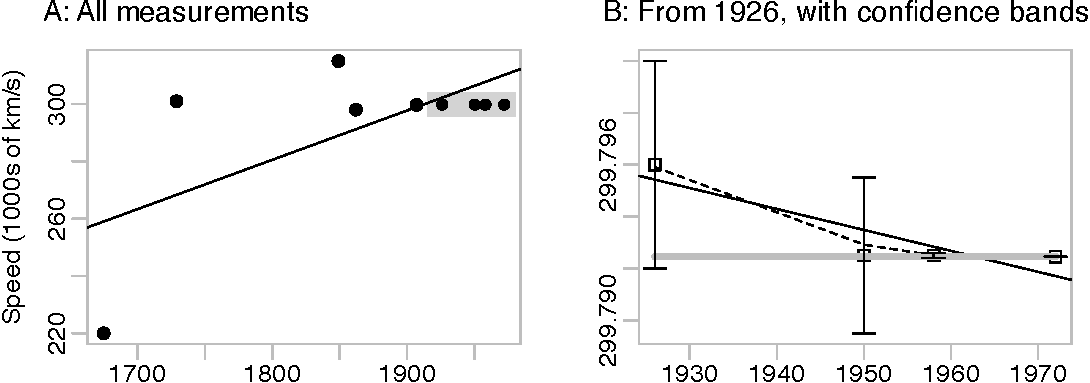
\includegraphics{09-covariate_files/figure-latex/plot-c-data-1.pdf}
\caption{\label{fig:plot-c-data}Successive speed of light estimates.
Error estimates are available for the 1855 and later
measurments. Panel B limits attention to measurements
made in 1926 and later. The line
was fitted with no adjustment for the very different error
estimates. The dashed curve, which incorporates
such adjustments, is statistically indistinguishable
from the red horizontal line.}
\end{figure}

Even if one were to accept Setterfield's manipulation of the data,
it makes no sense at all to fit either lines such as are shown, or
curves, to data values which have such very different
accuracies as those shown in the graphs. For the
measurements from 1862 onwards, estimates of accuracy are
available. Until 1950, each new estimate lay outside the
bounds for the previous estimate, indicating that these
were underestimates.

The right panel is limited to the points from 1926 and on,
marked off with the gray background on the left panel.

\hypertarget{global-mean-temperature-trends}{%
\section{Global mean temperature trends}\label{global-mean-temperature-trends}}

Figure \ref{fig:climate} plots global
\href{http://iridl.ldeo.columbia.edu/SOURCES/.NASA/.GISS/.GISSTEMP/.Global/.LOTI/}{air and sea surface temperature anomaly data}
against year. Anomalies, in hundredths of a degree centigrade, are
differences from the 1951-1980 global average. The grey curve plots
the average anomaly up to that point in time.

\begin{Shaded}
\begin{Highlighting}[]
\NormalTok{cap20 }\OtherTok{\textless{}{-}} \StringTok{"Anomalies (differences) in hundredths of a degree centigrade}
\StringTok{from global average temperatures over 1951{-}1980, plotted against year.}
\StringTok{The gray curve shows, for each year, the average anomaly up to that}
\StringTok{point in time.  The last year in which this lay below the gray line}
\StringTok{was 1962."}
\end{Highlighting}
\end{Shaded}

\begin{Shaded}
\begin{Highlighting}[]
\DocumentationTok{\#\# {-}{-}{-}{-} loti{-}smooth {-}{-}{-}{-}{-}{-}{-}{-}}
\FunctionTok{load}\NormalTok{(}\StringTok{\textquotesingle{}data/loti.RData\textquotesingle{}}\NormalTok{)}
\NormalTok{anomaly }\OtherTok{\textless{}{-}}\NormalTok{ loti[, }\StringTok{"J.D"}\NormalTok{]}
\NormalTok{num }\OtherTok{\textless{}{-}} \FunctionTok{seq}\NormalTok{(}\AttributeTok{along =}\NormalTok{ anomaly)}
\NormalTok{AVtodate }\OtherTok{\textless{}{-}} \FunctionTok{cumsum}\NormalTok{(anomaly)}\SpecialCharTok{/}\NormalTok{num}
\NormalTok{yr }\OtherTok{\textless{}{-}}\NormalTok{ loti}\SpecialCharTok{$}\NormalTok{Year}
\NormalTok{anomTxt }\OtherTok{\textless{}{-}} \StringTok{"Difference from baseline"}
\NormalTok{yl }\OtherTok{=} \FunctionTok{substitute}\NormalTok{(txt }\SpecialCharTok{*} \StringTok{" (0.01"} \SpecialCharTok{*}\NormalTok{ degree }\SpecialCharTok{*} \StringTok{"C)"}\NormalTok{,}
                  \FunctionTok{list}\NormalTok{(}\AttributeTok{txt=}\NormalTok{anomTxt))}
\FunctionTok{plot}\NormalTok{(yr, anomaly, }\AttributeTok{xlab =} \StringTok{"Year"}\NormalTok{, }\AttributeTok{ylab =} \FunctionTok{as.expression}\NormalTok{(yl))}
\FunctionTok{mtext}\NormalTok{(}\AttributeTok{side=}\DecValTok{3}\NormalTok{, }\AttributeTok{line=}\FloatTok{0.75}\NormalTok{,}
      \StringTok{"Global temperature differences from 1951{-}1980 global average"}\NormalTok{)}
\FunctionTok{lines}\NormalTok{(AVtodate }\SpecialCharTok{\textasciitilde{}}\NormalTok{ yr, }\AttributeTok{col =} \StringTok{"gray"}\NormalTok{, }\AttributeTok{lwd =} \DecValTok{2}\NormalTok{)}
\NormalTok{lastLessYr }\OtherTok{\textless{}{-}} \FunctionTok{max}\NormalTok{(yr[anomaly }\SpecialCharTok{\textless{}}\NormalTok{ AVtodate])}
\NormalTok{lastLessy }\OtherTok{\textless{}{-}}\NormalTok{ loti[}\FunctionTok{as.character}\NormalTok{(lastLessYr), }\StringTok{"J.D"}\NormalTok{]}
\NormalTok{yarrow }\OtherTok{\textless{}{-}}\NormalTok{ lastLessy }\SpecialCharTok{{-}} \FunctionTok{c}\NormalTok{(}\DecValTok{4}\NormalTok{, }\FloatTok{0.75}\NormalTok{) }\SpecialCharTok{*} \FunctionTok{strheight}\NormalTok{(}\StringTok{"O"}\NormalTok{)}
\FunctionTok{arrows}\NormalTok{(lastLessYr, yarrow[}\DecValTok{1}\NormalTok{], lastLessYr, yarrow[}\DecValTok{2}\NormalTok{],}
       \AttributeTok{col =} \StringTok{"gray"}\NormalTok{, }\AttributeTok{lwd =} \DecValTok{2}\NormalTok{)}
\end{Highlighting}
\end{Shaded}

\begin{figure}[H]
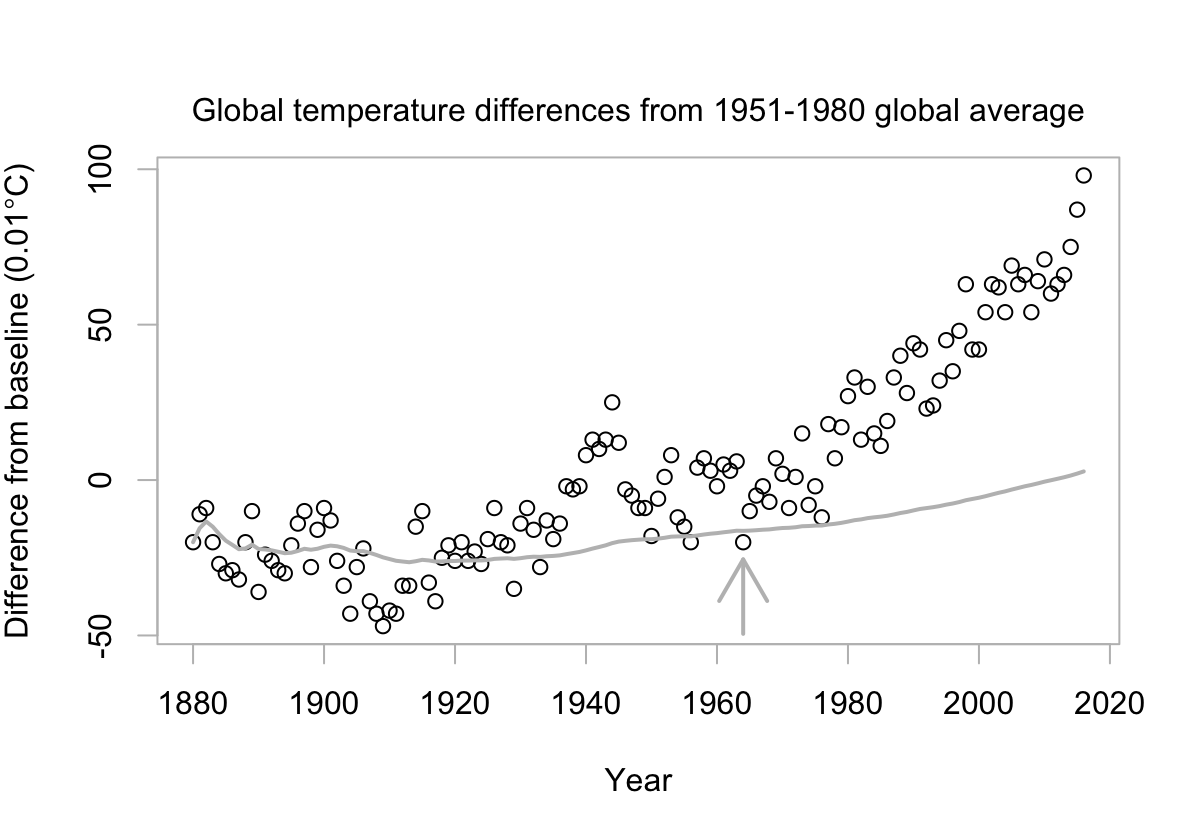
\includegraphics[width=0.8\linewidth]{09-covariate_files/figure-latex/climate-1} \caption{Anomalies (differences) in hundredths of a degree centigrade
from global average temperatures over 1951-1980, plotted against year.
The gray curve shows, for each year, the average anomaly up to that
point in time.  The last year in which this lay below the gray line
was 1962.}\label{fig:climate}
\end{figure}

Observe that 1964 was the last year in which the global
temperature fell below the average to that time.
For the 52 subsequent years (from 1965 to 2016 inclusive),
the global average was above the average up to that date. Under
the (false) assumption that global temperature is varying
randomly (and therefore independently) about a common mean,
the probability of this happening is 2\(^{-40}\) = 9.1
\(\times\) 10\(^{-13}\). A variation of this argument came
from a speaker on the Australian ABC Science Show on April
3 2011. Under any model that accounts for what are now
fairly well understood patterns of correlation over time,
the probability, while very small, is not that small!
Arguments that overstate the case for what is now a
well-established pattern of change are unhelpful

It is likewise nonsensical to fit a line to the cherry-picked
years 1998-2008, where the trend was relatively flat.

\hypertarget{the-critique-of-scientific-claims}{%
\chapter{The critique of scientific claims}\label{the-critique-of-scientific-claims}}

An ideal is that scientific processes will keep~to a minimum
the publication of claims that are not supported by evidence.
Like anything designed by humans, and put into practice by
humans, this is not precisely how it works in practice.
Notwithstanding peer review processes that are designed to
ensure that claims made in scientific papers withstand
careful scrutiny, the traps and fallacies described in these
notes, and more besides, are found in the scientific literature.
The effectiveness of the peer review process varies widely from
one area of science to another.

\hypertarget{what-results-can-be-trusted}{%
\section{What results can be trusted?}\label{what-results-can-be-trusted}}

Scientific processes work best when claims made by one scientist
or group of scientists attract widespread interest and critique
from the wider group of scientists who work in the same general
area. Examples are the May 2020 Lancet and New England Journal of
Medicine papers arguing that use of the drug hydroxychloroquine
as a treatment for Covid-19 was increasing patient deaths.\\
Issues with these papers were quickly identified because they
made claims that bore on an issue of major concern,~and attracted
attention from readers who carefully scrutinized their detailed
statements. They were quickly retracted.

Heavy reliance on the sharing of data and skills, and full use of
the benefits that modern technology has to offer, have been vital
to progress in such areas as earthquake science, the study of
viruses and vaccines, modelling of epidemics, and climate science.
This sharing of data and skills, and use of modern technology, also
helps in the critique of what has been published earlier.
Areas where there has not been the same impetus for change are much
more susceptible to the damage that arises from systems for funding
and publishing science that encourage the formal publication of
what would better be treated as preliminary results --- a first
stab at an answer. Publication of experimental results should not
be a once-for-all event, but a staged process that moves from
``this looks promising'' to ``has been independently replicated'',
and to post=publication critique.

Publication does not of itself validate scientific claims,
Rather, as stated in \citet{popper_1963}

\begin{quote}
Observations or experiments can be accepted as supporting a theory (or a hypothesis, or a scientific assertion) only if these observations or experiments are severe tests of the theory -- or in other words, only if they result from serious attempts to refute the theory.
\end{quote}

\hypertarget{a-look-at-what-can-go-wrong}{%
\section{A look at what can go wrong}\label{a-look-at-what-can-go-wrong}}

Fraud, though uncommon, happens more often than one might hope.
What is disturbing is the small number of scientists with
large numbers of papers that were retracted on account of
fraud. How were they able to get away with publishing so
many papers, usually with fraudulent data, before the
first identification of fraud that led to a checking of all
their work? \citet{ritchie2020science} (pp67-68) cites, as an
extreme example, the case of a Japanese anesthesiologist
with 183 retracted papers.

More common are mistakes in data collection, unacknowledged
sources of bias, hype, mistakes or~biases in the handling of
data and/or in data analysis, attaching a much higher
degree of certainty to~statistical evidence than the results
warrant, and selection effects. Selection effects can work
in various ways --- selection of a subset of data where
there appears to be an effect of~interest, choice of the
outcome variable and/or analysis approach that most nearly
gives the result that is wanted, and so on. In analysis of
data from experiments where two treatments are compared,
the common use of the arbitrary \(p <= 0.05\) criterion
(see the next subsection) as a cutoff for deciding what
will be published has the inevitable effect of selecting out,
in contexts where there was no difference of consequence
one in twenty of such results for publication. This adds
to other selection effects.

\hypertarget{the-case-of-eysenck-and-his-collaborators}{%
\section{The case of Eysenck and his collaborators}\label{the-case-of-eysenck-and-his-collaborators}}

At the time of his death in 1997, Eysenck was the living psychologist
most frequently cited in the peer-reviewed scientific literature.
Much of~his work was controversial in its time, with papers
containing ``questionable data and results so dramatic they beggared
belief'' {[}o2020famous{]}. He relied heavily on what has now been
identified heavily doctored data that was supplied to him by
German collaborator Grossarth-Maticek. Particularly egregious was
the claim that individuals with an identifiably cancer-prone personality
had a risk of dying from cancer that was as much as 121 times higher
than that of people with a ``healthy'' personality --- one of several
links that the duo~claimed to have found between personality and
mortality. Investigations into~Eysenck's work, including
collaborative work~with Grossarth-Maticek, are ongoing. Fourteen
papers have been retracted, and another 71 have received
``expressions of concern''. A large replication study conducted in
2004 found none of~the claimed links, apart from a modest link between
personality and cardiovascular disease.

\hypertarget{the-use-of-artificial-intelligence-to-detect-covid-19}{%
\section{The use of artificial intelligence to detect Covid-19}\label{the-use-of-artificial-intelligence-to-detect-covid-19}}

\citet{roberts2021common} identified an astonishing 320 papers and preprints
that appeared between 1 January 2020 to 3 October 2020, and which
describe the use of new machine learning models for the diagnosis of
COVID-19 from chest radiographic (CXR) and chest computed tomography
(CT) images. Quality screening reduced this~number to 62, which were
then examined in more detail. None of the 62 satisfied these more
detailed requirements, designed to check whether the algorithms used
had been shown to~be effective for~use in clinical practice. Among
other deficiencies, 48 did not complete any external validation, and
55 had a high risk of bias with respect to at least one of
participants, predictors, outcomes and analysis. In a popular account
of the results that appeared in New Scientist, \citet{roberts2021machine}
comments that, relative
to persisting to develop a model that will survive a rigorous
checking process and~might be used in practice, ``it is far easier
to~develop~a model with poor rigour and {[}apparent{]} excellent
performance and publish this.'' This is a damming indictment of
the way that large parts of the research and publication process
currently work. The public good would~be much better served
by a process that encourages researchers to persist until it
has been demonstrated that researchers have a model that meets
standards such as are set out in \citet{roberts2021common}. One may
hope that one result of this work will be to shift the research
and publication focus accordingly.

\hypertarget{laboratory-experimental-science-what-do-we-find}{%
\section{Laboratory experimental science --- what do~we find?}\label{laboratory-experimental-science-what-do-we-find}}

In the past several years, there has been a steady accumulation
of evidence that relates to the claim, in \citet{r19_ioannidis_2005},
that ``most published research findings are false''. Ioannidis
has in mind, not published results in general, but primarily
laboratory studies. Papers that have added to the
body of evidence that broadly support claims made in the
Ioannidis paper include:

\begin{itemize}
\tightlist
\item
  Amgen: Reproduced 6 only of 53 `landmark' cancer studies.

  \begin{itemize}
  \tightlist
  \item
    \citet{r23_begley_ellis_2012}
  \item
    \citet{r2_begley_2013} notes issues with the studies that failed
  \end{itemize}
\item
  Bayer: Main results from 19 of 65 `seminal' drug studies

  \begin{itemize}
  \tightlist
  \item
    NB, journal impact factor was not a good predictor!
  \item
    \citet{r9_prinz_schlange_asadullah_2011}
  \end{itemize}
\item
  fMRI studies: 57 of 134 papers (42\%) had \(\geq\) 1 case lacking
  check on separate test image.
  Another 14\%, unclear \ldots{}

  \begin{itemize}
  \tightlist
  \item
    \citet{r8_kriegeskorte_simmons_bellgowan_baker_2009}
  \end{itemize}
\end{itemize}

The psychological science community is further advanced in
addressing these issues that many other communities, with
The Center for Open Science (COS) taking a strong lead in
studies designed to document the extent of the issues.

Other Center for Open Science (COS) Projects have been:

\begin{itemize}
\tightlist
\item
  Many Labs --- reproduce 13 classical psych studies

  \begin{itemize}
  \tightlist
  \item
    Of 13 studies --- 10: successful, 1: weakly, 2: no!
  \item
    Plots show scatter across the 36 participating teams
  \item
    \citet{r7_klein_others_2014}
  \end{itemize}
\item
  Cancer Studies --- 50 ``most impactful'' from 2010-2012

  \begin{itemize}
  \tightlist
  \item
    \citet{r5_kaiser_2015}
  \end{itemize}
\end{itemize}

Details from other relevant studies are given in the
recent~book \citet{ritchie2020science} ``Science fictions: Exposing
fraud, bias, negligence and hype in science.''
Problems arise, primarily, in areas where relatively small
groups of scientists, with similar training and skills, work
independently. The critiques have limited relevance to
areas where the nature of the work forces collaboration
between scientists with diverse skills, widely across
different research groups.

Even with such checks as there are on published research, it is
clear that not everything that passes the peer review process
can be relied on. The case is far worse for claims made, often
for reasons of commercial gain, who have no~evidence at all for
the effectiveness of the therapy or remedy that they promote.

\hypertarget{the-reproducibility-psychology-project}{%
\section{The Reproducibility: Psychology project}\label{the-reproducibility-psychology-project}}

Figure \ref{fig:effect-size} summarizes evidence from
the Reproducibility: Psychology project \citep{r1_osc_EstRep2015}.
The effect size is the difference between the two means that
are to be compared, divided by the pooled standard deviation
for the two groups.

\begin{itemize}
\tightlist
\item
  It chose 100 studies (3 journals, 2008)
\item
  There was one replicate only of each study
\item
  Initial results: 39 agree + 24 ? ``similar'' + 37 fail
\end{itemize}

\begin{figure}[H]
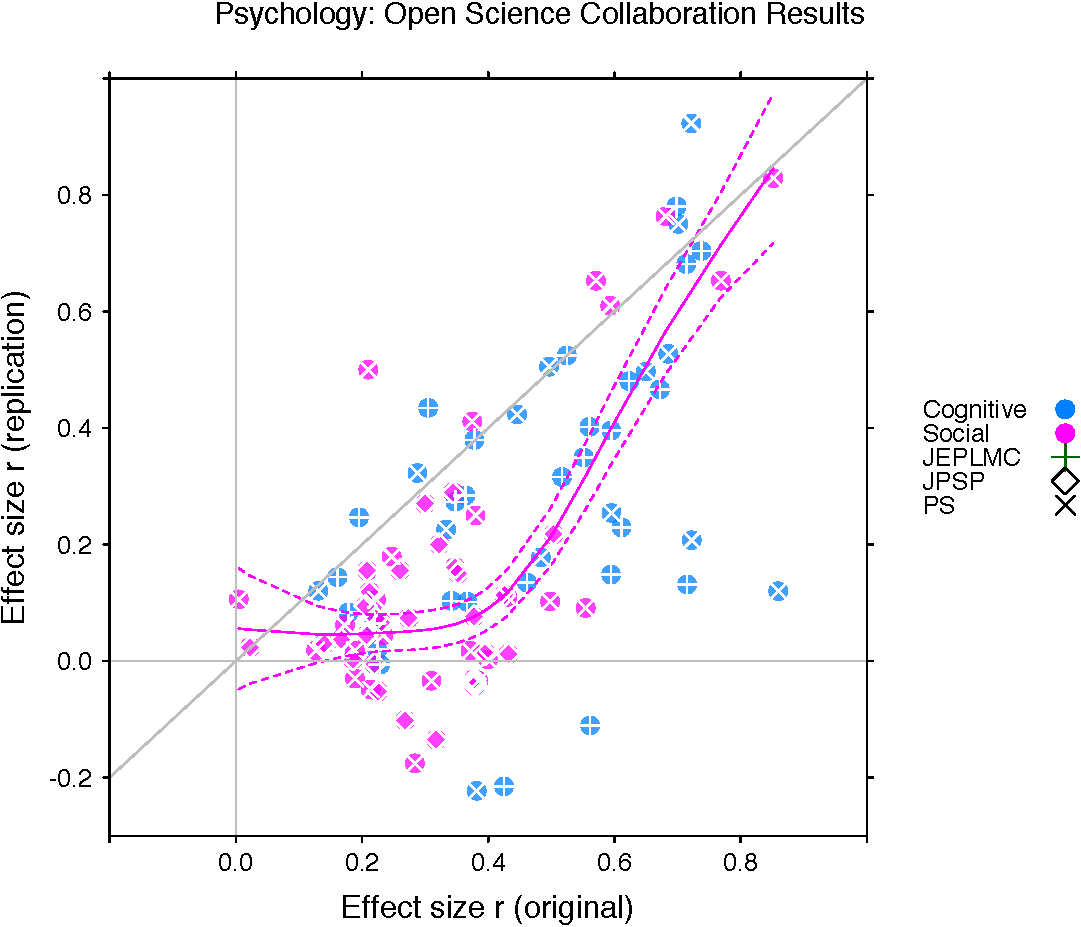
\includegraphics[width=0.7\linewidth]{10-science_files/figure-latex/effect-size-1} \caption{Psychology reproducibility project --- Effect sizes are
compared between the replication and the initial study.}\label{fig:effect-size}
\end{figure}

Notice that the effect size is almost always smaller for
the replication. A smooth curve, with confidence interval,
has been fitted for results in social psychology. Notice
that, for social psychology, it is only for an original
effect size greater than 0.4 that one starts to see a
positive correlation between the effect sizes for replicate
and original.

\hypertarget{when-science-and-commercial-interests-collide}{%
\section{When science and commercial interests collide}\label{when-science-and-commercial-interests-collide}}

\hypertarget{the-tobacco-and-fossil-fuel-industries}{%
\subsection*{The tobacco and fossil fuel industries}\label{the-tobacco-and-fossil-fuel-industries}}
\addcontentsline{toc}{subsection}{The tobacco and fossil fuel industries}

The tobacco industry has made extensive use of ``the science is not settled''
arguments in its efforts to dismiss the evidence that smoking causes lung cancer.
The goal has been to raise doubt, create confusion and undermine the science.
The same PR firms,~and the same researchers used to support these efforts
were later used in the attempt to undermine climate science.\footnote{\url{https://www.scientificamerican.com/article/tobacco-and-oil-industries-used-same-researchers-to-sway-public1/}\textgreater{}}

In spite of the support that has been available from the fossil
fuel industry for research that is critical of mainstream climate science
research, no substantially different alternative account has emerged, and
no climate change models have emerged that give results that are widely
different from the consensus. An interesting case is that of
Richard Muller's Berkeley Earth Surface Temperature Study (BEST),
with a large part of the funding coming from the right-wing billionaire
Charles Koch, known for funding climate skeptic groups such as the
Heartland Institute.

Richard Muller had been known for his skepticism, in part supported
by legitimate scientific concerns. He made headlines when he announced
his acceptance of what climate scientists had already been saying
for more than 15 years previous.
\textgreater{} After years of denying global warming, physicist Richard Muller now says ``global warming is real and humans are almost entirely the cause.''\footnote{\url{https://courses.seas.harvard.edu/climate/eli/Courses/global-change-debates/Sources/Hockeystick-global-temperature/more/Richard-Muller/Muller-is-a-believer-Hallelujah.pdf}\textgreater{}}

The broad sweep of work in climate science is, because it has survived
informed critique, and because of the diversity of contributing skills
and data, unusually secure. Details, especially as they affect what may
happen in individual countries, are subject to continual revision.

A particular issue is the role of the greenhouse gases, and of their
interactions with water vapour. Much larger than their direct effect
is the contribution that comes from their warming of the air in which
water vapour is present, allowing it to retain more vapour and trap
more heat). A standard denialist trump card has been to claim the
authority of scientists who have standing in their own areas for the
claim that the contribution of greenhouse gases is inconsequential
relative to that of water
vapour.\footnote{See \url{https://west.web.unc.edu/climate-change/} and
  \textless\textgreater{}}
The scientists involved are among a number who have fossil fuel
industry links, and have been willing to allow themselves to be
used as advocates for an industry that sees action on climate
change as a threat.\footnote{\url{https://insideclimatenews.org/news/12032015/leaked-email-reveals-whos-who-list-climate-denialists-merchants-of-doubt-oreskes-fred-singer-marc-morano-steve-milloy}}

\hypertarget{big-pharma}{%
\subsection*{Big Pharma}\label{big-pharma}}
\addcontentsline{toc}{subsection}{Big Pharma}

Between 1999 and 2019, opioid deaths in the United States increased
by a factor of six, to almost 50,000.

A large contributor has been the increased use of prescription
opioids. Purdue Pharma stands out for its aggressive marketing of
oxycodone, sold under the brand name OxyContin, arguing that
concerns over addiction and other dangers from the drugs were
overblown. In September 2019, Purdue Pharma declared bankruptcy,
facing significant liability in OxyContin and opioid addiction
lawsuits. Details of settlements are still being worked in the
courts.\footnote{ \url{https://topclassactions.com/lawsuit-settlements/open-lawsuit-settlements/opioids/purdue-opioid-addiction-class-action-settlement/}}

Strict regulations govern, in most countries, the approval~of
prescription drugs. Purdue Pharma exploited the much more
limited control over off-label use of approved drugs, i.e.,
use for purposes for which they have not received formal
approval, and for a time stayed under the radar.

Another scandal that demonstrates how drug companies can
sometimes work their way around the approval process
concerns the drug Vioxx, likewise marketed as a
painkiller.\citep{valentine2007timeline} Concerns that the
drug might be increasing the risk of heart attacks began
to~emerge in the months following its approval for use
in May 1999. By November 1, a study set up to investigate
these concerns reported 79 heart attacks out of 4000
among those taking the drug, as opposed to 41 among a
comparator group that was taking naproxen. The drug
continued on the market as the evidence against Vioxx
strengthened further. It was argued, with no evidence
to~back this up, that naproxen likely had a protective
effect. In any case, why allow Vioxx to go to~market
when naproxen was clearly carried less risk.

In September 2004,
when a colon-polyp prevention study showed that Vioxx
increased the risk of heart attack after 18 months,
Merck withdrew the drug. A Lancet paper that was
published later estimated that between 88,000 and
140,000 Americans had heart attacks from taking
Vioxx.\footnote{\citet{juni2004risk}} The increased risk continued
long after patients had ceased taking the drug.

\hypertarget{what-can-one-trust}{%
\subsection*{What can one trust?}\label{what-can-one-trust}}
\addcontentsline{toc}{subsection}{What can one trust?}

One may hope that checks on any new drug will be
stricter than was the case for Vioxx, that lessons
have been learned, that where in future drugs come
up for approval, checks will continue on possible
long-term effects. With fringe and quack medicines,
there are no such checks.

It has been interesting to follow approval processes
for Covid-19 vaccines. At the time of writing, the
Pfizer, Astrazena and Moderna vaccines have had, in
addition to their testing in clinical trials,
extra-ordinary levels of testing in clinical practice,
with risks that are small relative to the small risk
that we take ever time we cross a busy road.

\hypertarget{tricks-used-to-dismiss-established-scientific-results}{%
\section{Tricks used to dismiss established scientific results}\label{tricks-used-to-dismiss-established-scientific-results}}

The headings, and some of commentary, are adapted from an article by
Associate Professor Hassan Vally from La Trobe University,
\href{https://theconversation.com/5-ways-to-spot-if-someone-is-trying-to-mislead-you-when-it-comes-to-science-138814?utm_medium=email\&utm_campaign=Latest\%20from\%20The\%20Conversation\%20for\%20March\%209\%202021\%20-\%201883318379\&utm_content=Latest\%20from\%20The\%20Conversation\%20for\%20March\%209\%202021\%20-\%201883318379+CID_6009c8d7af2a01f376a88d0491598cfa\&utm_source=campaign_monitor\&utm_term=5\%20ways\%20to\%20spot\%20if\%20someone\%20is\%20trying\%20to\%20mislead\%20you\%20when\%20it\%20comes\%20to\%20science}{that appeared in \emph{The Conversation}}\footnote{\url{https://theconversation.com/5-ways-to-spot-if-someone-is-trying-to-mislead-you-when-it-comes-to-science-138814?utm_medium=email\&utm_campaign=Latest\%20from\%20The\%20Conversation\%20for\%20March\%209\%202021\%20-\%201883318379\&utm_content=Latest\%20from\%20The\%20Conversation\%20for\%20March\%209\%202021\%20-\%201883318379+CID_6009c8d7af2a01f376a88d0491598cfa\&utm_source=campaign_monitor\&utm_term=5\%20ways\%20to\%20spot\%20if\%20someone\%20is\%20trying\%20to\%20mislead\%20you\%20when\%20it\%20comes\%20to\%20science}}

\begin{enumerate}
\def\labelenumi{\arabic{enumi}.}
\tightlist
\item
  ``The `us versus them' narrative''\\
  The powers that be are trying to deceive us." Ask who is
  making real attempt to deceive --- commercial interest groups,
  peddlers of quack treatments, influence peddlers, . . .
\item
  `I'm not a scientist, but\ldots{}'
  Meaning perhaps: ``I'm not a scientist, but that does not stop me
  making an authoritative pronouncement that flies in the face of
  established results.''
  Or: ``I know what the science says, but I'm keeping an open mind''.\\
  Politicians are among the most frequent offenders.
\item
  Reference to `the science not being settled'\\
  There are of course times when the science is not settled, and when this is
  the case, one can expect scientists to openly argue different points of view
  based on the evidence available. Or, what has come to be accepted wisdom
  may turn out to be wrong or in need of substantial revision. But challenges
  to~the accepted wisdom have to be carefully argued, and themselves survive
  informed critique.
\item
  Overly simplistic explanations\\
  Oversimplifications and generalizations are central to many conspiracy theory
  arguments. Science is often messy, complex and full of nuance. The truth can
  be much harder to explain, and can sometimes sound less plausible, than a
  simple but incorrect explanation. Use of simplistic statistical arguments
  is common, e.g., fit a line to the cherry-picked years 1998-2008, ignoring
  year to year correlation as well as influences that operate over longer time
  periods.
\item
  Cherry-picking\\
  One is not entitled to choose one study over another just because it aligns
  with what you prefer to believe. This is not how science works.\\
  Not all studies are equal; some provide much stronger evidence than others.
  The way that choices are made has to stand up to critical scrutiny.
\end{enumerate}

\hypertarget{further-reading-books-videos-and-websites}{%
\chapter*{Further reading --- books, videos, and websites}\label{further-reading-books-videos-and-websites}}
\addcontentsline{toc}{chapter}{Further reading --- books, videos, and websites}

The books noted have all been referred to in the text.

\begin{itemize}
\tightlist
\item
  \citet{kahneman_2013} . Thinking, fast and slow.

  \begin{itemize}
  \tightlist
  \item
    \href{https://www.youtube.com/watch?v=PirFrDVRBo4}{Interview with Kahneman}\footnote{\url{https://www.youtube.com/watch?v=PirFrDVRBo4}}
  \item
    \href{https://www.youtube.com/watch?v=uqXVAo7dVRU\&t=28s}{A brief animated overview of some key points}\footnote{\url{https://www.youtube.com/watch?v=uqXVAo7dVRU\&t=28s}}
  \end{itemize}
\item
  \citet{smith-sd} . Standard Deviations: Flawed Assumptions, Tortured Data, and Other Ways to Lie with Statistics

  \begin{itemize}
  \tightlist
  \item
    \href{http://www.garysmithn.com/standard-deviations.html}{Brian Lehrer interview with Smith}\footnote{\url{http://www.garysmithn.com/standard-deviations.html}}
  \end{itemize}
\item
  \citet{ellenberg_2015} . How not to be wrong.

  \begin{itemize}
  \tightlist
  \item
    \href{http://www.thelavinagency.com/news/new-videos-jordan-ellenberg-runs-the-numbers}{There are links to several Ellenberg video clips}\footnote{\url{http://www.thelavinagency.com/news/new-videos-jordan-ellenberg-runs-the-numbers}}
  \end{itemize}
\item
  \citet{levitin_2016} . A field guide to lies and statistics.
\item
  \citet{nisbett} . Tools for smart thinking.
\item
  \citet{cairo_2013} . The functional art: an introduction to information
  graphics and visualization.
\item
  \citet{ritchie2020science} . Science fictions: Exposing fraud, bias,
  negligence and hype in science.
\item
  \href{http://www.bbc.co.uk/editorialguidelines/guidance/reporting-statistics}{BBC links to helpful web resources}\footnote{\url{http://www.bbc.co.uk/editorialguidelines/guidance/reporting-statistics}}
\end{itemize}

  \bibliography{book.bib,packages.bib,dataSense.bib}

\end{document}
